\documentclass[twoside]{book}

% Packages required by doxygen
\usepackage{fixltx2e}
\usepackage{calc}
\usepackage{doxygen}
\usepackage[export]{adjustbox} % also loads graphicx
\usepackage{graphicx}
\usepackage[utf8]{inputenc}
\usepackage{makeidx}
\usepackage{multicol}
\usepackage{multirow}
\PassOptionsToPackage{warn}{textcomp}
\usepackage{textcomp}
\usepackage[nointegrals]{wasysym}
\usepackage[table]{xcolor}

% Font selection
\usepackage[T1]{fontenc}
\usepackage[scaled=.90]{helvet}
\usepackage{courier}
\usepackage{amssymb}
\usepackage{sectsty}
\renewcommand{\familydefault}{\sfdefault}
\allsectionsfont{%
  \fontseries{bc}\selectfont%
  \color{darkgray}%
}
\renewcommand{\DoxyLabelFont}{%
  \fontseries{bc}\selectfont%
  \color{darkgray}%
}
\newcommand{\+}{\discretionary{\mbox{\scriptsize$\hookleftarrow$}}{}{}}

% Page & text layout
\usepackage{geometry}
\geometry{%
  a4paper,%
  top=2.5cm,%
  bottom=2.5cm,%
  left=2.5cm,%
  right=2.5cm%
}
\tolerance=750
\hfuzz=15pt
\hbadness=750
\setlength{\emergencystretch}{15pt}
\setlength{\parindent}{0cm}
\setlength{\parskip}{0.2cm}
\makeatletter
\renewcommand{\paragraph}{%
  \@startsection{paragraph}{4}{0ex}{-1.0ex}{1.0ex}{%
    \normalfont\normalsize\bfseries\SS@parafont%
  }%
}
\renewcommand{\subparagraph}{%
  \@startsection{subparagraph}{5}{0ex}{-1.0ex}{1.0ex}{%
    \normalfont\normalsize\bfseries\SS@subparafont%
  }%
}
\makeatother

% Headers & footers
\usepackage{fancyhdr}
\pagestyle{fancyplain}
\fancyhead[LE]{\fancyplain{}{\bfseries\thepage}}
\fancyhead[CE]{\fancyplain{}{}}
\fancyhead[RE]{\fancyplain{}{\bfseries\leftmark}}
\fancyhead[LO]{\fancyplain{}{\bfseries\rightmark}}
\fancyhead[CO]{\fancyplain{}{}}
\fancyhead[RO]{\fancyplain{}{\bfseries\thepage}}
\fancyfoot[LE]{\fancyplain{}{}}
\fancyfoot[CE]{\fancyplain{}{}}
\fancyfoot[RE]{\fancyplain{}{\bfseries\scriptsize Generated on Tue Oct 27 2015 14\+:23\+:59 for D\+N\+N by Doxygen }}
\fancyfoot[LO]{\fancyplain{}{\bfseries\scriptsize Generated on Tue Oct 27 2015 14\+:23\+:59 for D\+N\+N by Doxygen }}
\fancyfoot[CO]{\fancyplain{}{}}
\fancyfoot[RO]{\fancyplain{}{}}
\renewcommand{\footrulewidth}{0.4pt}
\renewcommand{\chaptermark}[1]{%
  \markboth{#1}{}%
}
\renewcommand{\sectionmark}[1]{%
  \markright{\thesection\ #1}%
}

% Indices & bibliography
\usepackage{natbib}
\usepackage[titles]{tocloft}
\setcounter{tocdepth}{3}
\setcounter{secnumdepth}{5}
\makeindex

% Hyperlinks (required, but should be loaded last)
\usepackage{ifpdf}
\ifpdf
  \usepackage[pdftex,pagebackref=true]{hyperref}
\else
  \usepackage[ps2pdf,pagebackref=true]{hyperref}
\fi
\hypersetup{%
  colorlinks=true,%
  linkcolor=blue,%
  citecolor=blue,%
  unicode%
}

% Custom commands
\newcommand{\clearemptydoublepage}{%
  \newpage{\pagestyle{empty}\cleardoublepage}%
}


%===== C O N T E N T S =====

\begin{document}

% Titlepage & ToC
\hypersetup{pageanchor=false,
             bookmarks=true,
             bookmarksnumbered=true,
             pdfencoding=unicode
            }
\pagenumbering{roman}
\begin{titlepage}
\vspace*{7cm}
\begin{center}%
{\Large D\+N\+N \\[1ex]\large 1.\+0 }\\
\vspace*{1cm}
{\large Generated by Doxygen 1.8.9.1}\\
\vspace*{0.5cm}
{\small Tue Oct 27 2015 14:23:59}\\
\end{center}
\end{titlepage}
\clearemptydoublepage
\tableofcontents
\clearemptydoublepage
\pagenumbering{arabic}
\hypersetup{pageanchor=true}

%--- Begin generated contents ---
\chapter{riema\+N\+N}
\label{md__r_e_a_d_m_e}
\hypertarget{md__r_e_a_d_m_e}{}
This work has been partially funded by the French cooperative project T\+I\+M\+C\+O, Pôle de Compétitivité Systematic (F\+U\+I 13). 
\chapter{Class Index}
\section{Class List}
Here are the classes, structs, unions and interfaces with brief descriptions\+:\begin{DoxyCompactList}
\item\contentsline{section}{\hyperlink{struct_conv_layer_params}{Conv\+Layer\+Params} }{\pageref{struct_conv_layer_params}}{}
\item\contentsline{section}{\hyperlink{struct_params}{Params} }{\pageref{struct_params}}{}
\item\contentsline{section}{\hyperlink{struct_pool_layer_params}{Pool\+Layer\+Params} }{\pageref{struct_pool_layer_params}}{}
\end{DoxyCompactList}

\chapter{File Index}
\section{File List}
Here is a list of all documented files with brief descriptions\+:\begin{DoxyCompactList}
\item\contentsline{section}{\hyperlink{conv__fd_test_8cpp}{conv\+\_\+fd\+Test.\+cpp} \\*Main function for testing backpropagation for convolutional neural networks }{\pageref{conv__fd_test_8cpp}}{}
\item\contentsline{section}{\hyperlink{convnet_8cpp}{convnet.\+cpp} \\*Main function for launching experiments with convolutional neural networks }{\pageref{convnet_8cpp}}{}
\item\contentsline{section}{\hyperlink{convnet__sp_8cpp}{convnet\+\_\+sp.\+cpp} \\*Main function for launching experiments with convolutional neural networks and sparse network }{\pageref{convnet__sp_8cpp}}{}
\item\contentsline{section}{\hyperlink{nn__ops_8hpp}{nn\+\_\+ops.\+hpp} \\*Implementation of the functions required for neural networks }{\pageref{nn__ops_8hpp}}{}
\item\contentsline{section}{\hyperlink{nn__ops__conv_8hpp}{nn\+\_\+ops\+\_\+conv.\+hpp} \\*Implementation of the functions required for convolutional neural networks }{\pageref{nn__ops__conv_8hpp}}{}
\item\contentsline{section}{\hyperlink{nn__ops__sp__conv_8hpp}{nn\+\_\+ops\+\_\+sp\+\_\+conv.\+hpp} \\*Implementation of the functions required for neural networks }{\pageref{nn__ops__sp__conv_8hpp}}{}
\item\contentsline{section}{\hyperlink{riemann_8cpp}{riemann.\+cpp} \\*Main function for launching experiments with neural networks }{\pageref{riemann_8cpp}}{}
\item\contentsline{section}{\hyperlink{utils_8hpp}{utils.\+hpp} \\*Implementation of auxiliary functions required for dataset loading and outputting }{\pageref{utils_8hpp}}{}
\item\contentsline{section}{{\bfseries utils\+\_\+conv.\+hpp} }{\pageref{utils__conv_8hpp}}{}
\end{DoxyCompactList}

\chapter{Class Documentation}
\hypertarget{struct_conv_layer_params}{}\section{Conv\+Layer\+Params Struct Reference}
\label{struct_conv_layer_params}\index{Conv\+Layer\+Params@{Conv\+Layer\+Params}}
\subsection*{Public Attributes}
\begin{DoxyCompactItemize}
\item 
\hypertarget{struct_conv_layer_params_a5c287b89252587f4ca47ff1f96be0417}{}unsigned {\bfseries Hf}\label{struct_conv_layer_params_a5c287b89252587f4ca47ff1f96be0417}

\item 
\hypertarget{struct_conv_layer_params_a1f3c7c581843bec279636537cc23497f}{}unsigned {\bfseries padding}\label{struct_conv_layer_params_a1f3c7c581843bec279636537cc23497f}

\item 
\hypertarget{struct_conv_layer_params_a655b47437125d27c52912f888c21488e}{}unsigned {\bfseries n\+\_\+filter}\label{struct_conv_layer_params_a655b47437125d27c52912f888c21488e}

\item 
\hypertarget{struct_conv_layer_params_a413880283a4f5fcb4bd772093d0aa372}{}unsigned {\bfseries stride}\label{struct_conv_layer_params_a413880283a4f5fcb4bd772093d0aa372}

\item 
\hypertarget{struct_conv_layer_params_af95630e4f19fbdd31c71d5f0266ceb89}{}unsigned {\bfseries filter\+\_\+size}\label{struct_conv_layer_params_af95630e4f19fbdd31c71d5f0266ceb89}

\item 
\hypertarget{struct_conv_layer_params_a9b76f4b76599348c8ea5045ba258d315}{}unsigned {\bfseries N}\label{struct_conv_layer_params_a9b76f4b76599348c8ea5045ba258d315}

\end{DoxyCompactItemize}


The documentation for this struct was generated from the following file\+:\begin{DoxyCompactItemize}
\item 
utils\+\_\+conv.\+hpp\end{DoxyCompactItemize}

\hypertarget{struct_params}{}\section{Params Struct Reference}
\label{struct_params}\index{Params@{Params}}
\subsection*{Public Attributes}
\begin{DoxyCompactItemize}
\item 
\hypertarget{struct_params_a88746ed42fe391f830c403cedb1193a5}{}std\+::string {\bfseries algo}\label{struct_params_a88746ed42fe391f830c403cedb1193a5}

\item 
\hypertarget{struct_params_a2d2a66ab390c4dda9c26e17ddb2055f0}{}std\+::vector$<$ unsigned $>$ {\bfseries nn\+\_\+arch}\label{struct_params_a2d2a66ab390c4dda9c26e17ddb2055f0}

\item 
\hypertarget{struct_params_a415bd96d2d7547cd67080839b2836a31}{}unsigned {\bfseries n\+\_\+params}\label{struct_params_a415bd96d2d7547cd67080839b2836a31}

\item 
\hypertarget{struct_params_a86164c8cf081484b7cb75a917da664a3}{}std\+::string {\bfseries act\+\_\+func\+\_\+name}\label{struct_params_a86164c8cf081484b7cb75a917da664a3}

\item 
\hypertarget{struct_params_a3750fc7b5585673e143de83f279f8b38}{}double {\bfseries ratio\+\_\+train}\label{struct_params_a3750fc7b5585673e143de83f279f8b38}

\item 
\hypertarget{struct_params_aa8dc3d413bb25e95185ca10679179363}{}bool {\bfseries schedule\+\_\+flag}\label{struct_params_aa8dc3d413bb25e95185ca10679179363}

\item 
\hypertarget{struct_params_ad27067c6caa54936cd94fff83d1ce834}{}double {\bfseries eta}\label{struct_params_ad27067c6caa54936cd94fff83d1ce834}

\item 
\hypertarget{struct_params_a18696b8c8f4bd37804d30fb60983aca8}{}double {\bfseries eta\+\_\+min}\label{struct_params_a18696b8c8f4bd37804d30fb60983aca8}

\item 
\hypertarget{struct_params_af70cb3045ba2b74208ab7ae5befe8665}{}bool {\bfseries adaptive\+\_\+flag}\label{struct_params_af70cb3045ba2b74208ab7ae5befe8665}

\item 
\hypertarget{struct_params_af01f5ffeeb3af21cf1740307a276d0af}{}bool {\bfseries dropout\+\_\+flag}\label{struct_params_af01f5ffeeb3af21cf1740307a276d0af}

\item 
\hypertarget{struct_params_ad67729b385fdf1f7f192d99757ef2c17}{}double {\bfseries dropout\+\_\+prob}\label{struct_params_ad67729b385fdf1f7f192d99757ef2c17}

\item 
\hypertarget{struct_params_a08be2f30032fa9d6020e41ef22590cc3}{}bool {\bfseries dropout\+\_\+eval}\label{struct_params_a08be2f30032fa9d6020e41ef22590cc3}

\item 
\hypertarget{struct_params_ae641b3e0b2380c5c53e59debc1c6d1d7}{}unsigned {\bfseries train\+\_\+minibatch\+\_\+size}\label{struct_params_ae641b3e0b2380c5c53e59debc1c6d1d7}

\item 
\hypertarget{struct_params_adab70c763eff0adace2f30c7e05a608e}{}unsigned {\bfseries valid\+\_\+minibatch\+\_\+size}\label{struct_params_adab70c763eff0adace2f30c7e05a608e}

\item 
\hypertarget{struct_params_a1c10502d57f7e4604375cea5bd1c2311}{}unsigned {\bfseries minibatch\+\_\+size}\label{struct_params_a1c10502d57f7e4604375cea5bd1c2311}

\item 
\hypertarget{struct_params_aa29bc4541da70da115f131d7d7c31bf0}{}double {\bfseries metric\+\_\+gamma}\label{struct_params_aa29bc4541da70da115f131d7d7c31bf0}

\item 
\hypertarget{struct_params_a667c5cc706c74d77742af25039c3da2f}{}bool {\bfseries init\+\_\+metric\+\_\+id}\label{struct_params_a667c5cc706c74d77742af25039c3da2f}

\item 
\hypertarget{struct_params_af4864610ddc8cd31352d6b4da48e8c98}{}unsigned {\bfseries n\+\_\+epoch}\label{struct_params_af4864610ddc8cd31352d6b4da48e8c98}

\item 
\hypertarget{struct_params_a9d6681cc4e8768335e76629dcfb802ee}{}double {\bfseries matrix\+\_\+reg}\label{struct_params_a9d6681cc4e8768335e76629dcfb802ee}

\item 
\hypertarget{struct_params_ae982e63ffc004fdaf158fa64c9385fe3}{}unsigned {\bfseries sparsity}\label{struct_params_ae982e63ffc004fdaf158fa64c9385fe3}

\item 
\hypertarget{struct_params_a72e86074f4b8b5d6e99302d636827b86}{}double {\bfseries imp\+\_\+sampling\+\_\+ratio}\label{struct_params_a72e86074f4b8b5d6e99302d636827b86}

\item 
\hypertarget{struct_params_ac5bec714c3d890dd6808d96678e54457}{}bool {\bfseries invert\+\_\+pixel}\label{struct_params_ac5bec714c3d890dd6808d96678e54457}

\item 
\hypertarget{struct_params_a2fe88a016e5fc3db122ad43ff46a9366}{}unsigned {\bfseries img\+\_\+width}\label{struct_params_a2fe88a016e5fc3db122ad43ff46a9366}

\item 
\hypertarget{struct_params_a4a289ba06081d379eaad93b68c1daeb6}{}unsigned {\bfseries img\+\_\+height}\label{struct_params_a4a289ba06081d379eaad93b68c1daeb6}

\item 
\hypertarget{struct_params_a368dc5433583185b76e98435948161d2}{}unsigned {\bfseries img\+\_\+depth}\label{struct_params_a368dc5433583185b76e98435948161d2}

\item 
\hypertarget{struct_params_a0512c42d1327df82c62cd88d34137625}{}unsigned {\bfseries conv\+\_\+\+Hf1}\label{struct_params_a0512c42d1327df82c62cd88d34137625}

\item 
\hypertarget{struct_params_aaed9e83165b2a44dcf8e4ded37000e8c}{}unsigned {\bfseries conv\+\_\+\+Hf2}\label{struct_params_aaed9e83165b2a44dcf8e4ded37000e8c}

\item 
\hypertarget{struct_params_aa64248f279cfe32861bf133b7fc52b61}{}unsigned {\bfseries conv\+\_\+padding}\label{struct_params_aa64248f279cfe32861bf133b7fc52b61}

\item 
\hypertarget{struct_params_ae5462e2605946bae12c9479750457077}{}unsigned {\bfseries conv\+\_\+n\+\_\+filter}\label{struct_params_ae5462e2605946bae12c9479750457077}

\item 
\hypertarget{struct_params_a795bdcfe241f733d8359651f3713bfd9}{}unsigned {\bfseries conv\+\_\+stride1}\label{struct_params_a795bdcfe241f733d8359651f3713bfd9}

\item 
\hypertarget{struct_params_a65d8892248a07830ea1e4b04c51dbe81}{}unsigned {\bfseries conv\+\_\+stride2}\label{struct_params_a65d8892248a07830ea1e4b04c51dbe81}

\item 
\hypertarget{struct_params_a44ef27626e058f39bfa46a18a314eb0f}{}std\+::string {\bfseries regularizer}\label{struct_params_a44ef27626e058f39bfa46a18a314eb0f}

\item 
\hypertarget{struct_params_a3b185182fe39d3438ec461f9633b52c5}{}double {\bfseries lambda}\label{struct_params_a3b185182fe39d3438ec461f9633b52c5}

\item 
\hypertarget{struct_params_a0232026c0c0c395c0b1028f6129a97a5}{}bool {\bfseries minilog\+\_\+flag}\label{struct_params_a0232026c0c0c395c0b1028f6129a97a5}

\item 
\hypertarget{struct_params_ab5d70ea1f72a179aa3f50d6691ab3b1a}{}std\+::string {\bfseries dir\+\_\+path}\label{struct_params_ab5d70ea1f72a179aa3f50d6691ab3b1a}

\item 
\hypertarget{struct_params_aef14dda21219d65734adc08971102b0c}{}std\+::string {\bfseries exp\+\_\+desc}\label{struct_params_aef14dda21219d65734adc08971102b0c}

\item 
\hypertarget{struct_params_aaba0842db31c4079652abae6ef06b48d}{}std\+::string {\bfseries file\+\_\+path}\label{struct_params_aaba0842db31c4079652abae6ef06b48d}

\item 
\hypertarget{struct_params_ac583aa2ea2aa9d9c341cedbaf1bd583a}{}unsigned {\bfseries run\+\_\+id}\label{struct_params_ac583aa2ea2aa9d9c341cedbaf1bd583a}

\item 
\hypertarget{struct_params_aad6e1417ee38b5d4cc5ef879d4b463c5}{}unsigned {\bfseries seed}\label{struct_params_aad6e1417ee38b5d4cc5ef879d4b463c5}

\end{DoxyCompactItemize}


The documentation for this struct was generated from the following file\+:\begin{DoxyCompactItemize}
\item 
\hyperlink{utils_8hpp}{utils.\+hpp}\end{DoxyCompactItemize}

\hypertarget{struct_pool_layer_params}{}\section{Pool\+Layer\+Params Struct Reference}
\label{struct_pool_layer_params}\index{Pool\+Layer\+Params@{Pool\+Layer\+Params}}
\subsection*{Public Attributes}
\begin{DoxyCompactItemize}
\item 
\hypertarget{struct_pool_layer_params_a3a246dae600ef42be216a6b49486ed25}{}unsigned {\bfseries Hf}\label{struct_pool_layer_params_a3a246dae600ef42be216a6b49486ed25}

\item 
\hypertarget{struct_pool_layer_params_ad8dd2860fdcb3a9ec00fe945555224cc}{}unsigned {\bfseries padding}\label{struct_pool_layer_params_ad8dd2860fdcb3a9ec00fe945555224cc}

\item 
\hypertarget{struct_pool_layer_params_a161de5e8ba3c56cb2af6c42b80996877}{}unsigned {\bfseries stride}\label{struct_pool_layer_params_a161de5e8ba3c56cb2af6c42b80996877}

\item 
\hypertarget{struct_pool_layer_params_a897d646200ed4f01dc43045a8b74ba85}{}unsigned {\bfseries filter\+\_\+size}\label{struct_pool_layer_params_a897d646200ed4f01dc43045a8b74ba85}

\item 
\hypertarget{struct_pool_layer_params_acaa63212cc48f33f27b09cbb30806396}{}unsigned {\bfseries N}\label{struct_pool_layer_params_acaa63212cc48f33f27b09cbb30806396}

\end{DoxyCompactItemize}


The documentation for this struct was generated from the following file\+:\begin{DoxyCompactItemize}
\item 
utils\+\_\+conv.\+hpp\end{DoxyCompactItemize}

\chapter{File Documentation}
\hypertarget{conv__fd_test_8cpp}{}\section{conv\+\_\+fd\+Test.\+cpp File Reference}
\label{conv__fd_test_8cpp}\index{conv\+\_\+fd\+Test.\+cpp@{conv\+\_\+fd\+Test.\+cpp}}


main function for testing backpropagation for convolutional neural networks  


{\ttfamily \#include \char`\"{}utils.\+hpp\char`\"{}}\\*
{\ttfamily \#include \char`\"{}utils\+\_\+conv.\+hpp\char`\"{}}\\*
{\ttfamily \#include \char`\"{}nn\+\_\+ops\+\_\+conv.\+hpp\char`\"{}}\\*
Include dependency graph for conv\+\_\+fd\+Test.\+cpp\+:
\nopagebreak
\begin{figure}[H]
\begin{center}
\leavevmode
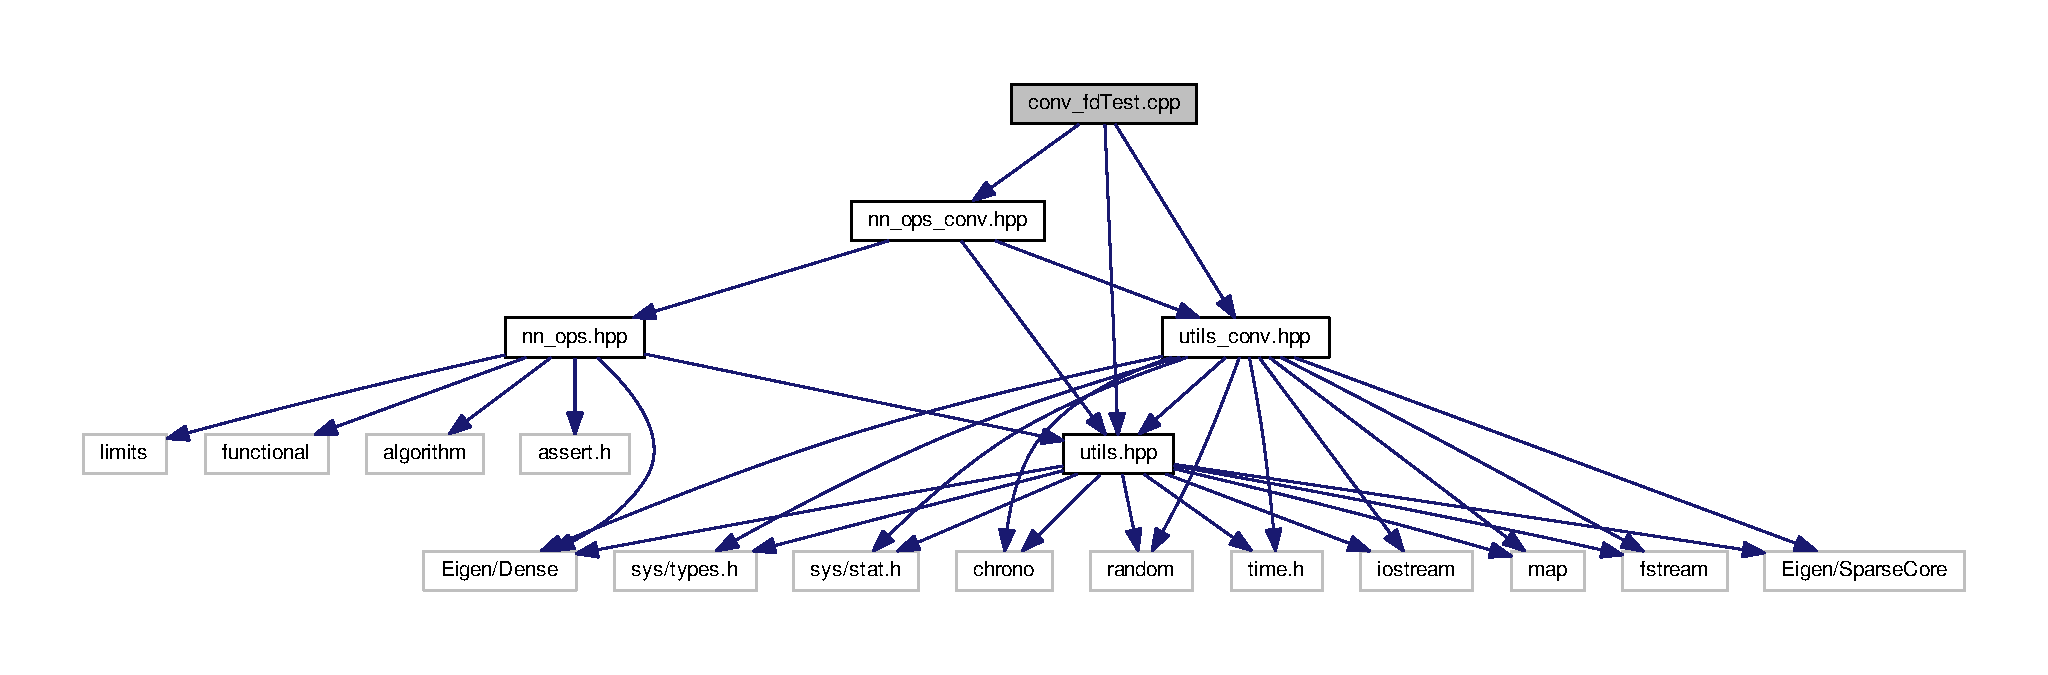
\includegraphics[width=350pt]{conv__fd_test_8cpp__incl}
\end{center}
\end{figure}
\subsection*{Functions}
\begin{DoxyCompactItemize}
\item 
\hypertarget{conv__fd_test_8cpp_a0ddf1224851353fc92bfbff6f499fa97}{}int {\bfseries main} (int argc, char $\ast$argv\mbox{[}$\,$\mbox{]})\label{conv__fd_test_8cpp_a0ddf1224851353fc92bfbff6f499fa97}

\end{DoxyCompactItemize}


\subsection{Detailed Description}
main function for testing backpropagation for convolutional neural networks 

\begin{DoxyAuthor}{Author}
Gaetan Marceau Caron \& Yann Ollivier 
\end{DoxyAuthor}
\begin{DoxyVersion}{Version}
1.\+0 
\end{DoxyVersion}

\hypertarget{convnet_8cpp}{}\section{convnet.\+cpp File Reference}
\label{convnet_8cpp}\index{convnet.\+cpp@{convnet.\+cpp}}


main function for launching experiments with convolutional neural networks  


{\ttfamily \#include \char`\"{}utils.\+hpp\char`\"{}}\\*
{\ttfamily \#include \char`\"{}utils\+\_\+conv.\+hpp\char`\"{}}\\*
{\ttfamily \#include \char`\"{}nn\+\_\+ops\+\_\+conv.\+hpp\char`\"{}}\\*
Include dependency graph for convnet.\+cpp\+:
\nopagebreak
\begin{figure}[H]
\begin{center}
\leavevmode
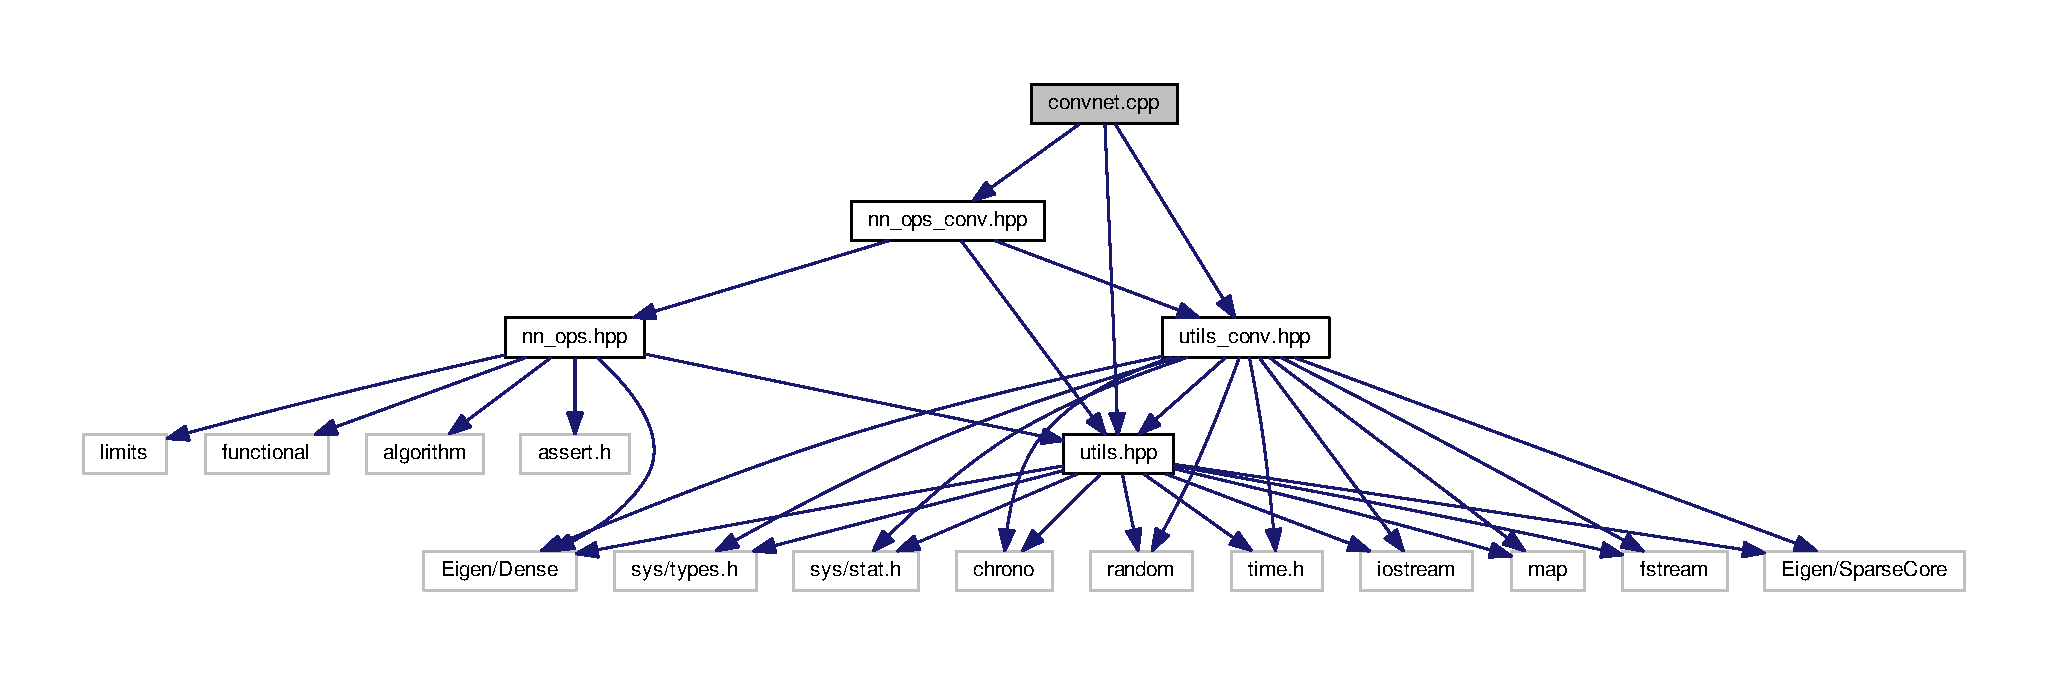
\includegraphics[width=350pt]{convnet_8cpp__incl}
\end{center}
\end{figure}
\subsection*{Functions}
\begin{DoxyCompactItemize}
\item 
\hypertarget{convnet_8cpp_a0ddf1224851353fc92bfbff6f499fa97}{}int {\bfseries main} (int argc, char $\ast$argv\mbox{[}$\,$\mbox{]})\label{convnet_8cpp_a0ddf1224851353fc92bfbff6f499fa97}

\end{DoxyCompactItemize}


\subsection{Detailed Description}
main function for launching experiments with convolutional neural networks 

\begin{DoxyAuthor}{Author}
Gaetan Marceau Caron \& Yann Ollivier 
\end{DoxyAuthor}
\begin{DoxyVersion}{Version}
1.\+0 
\end{DoxyVersion}

\hypertarget{convnet__sp_8cpp}{}\section{convnet\+\_\+sp.\+cpp File Reference}
\label{convnet__sp_8cpp}\index{convnet\+\_\+sp.\+cpp@{convnet\+\_\+sp.\+cpp}}


main function for launching experiments with convolutional neural networks and sparse network  


{\ttfamily \#include \char`\"{}utils.\+hpp\char`\"{}}\\*
{\ttfamily \#include \char`\"{}nn\+\_\+ops\+\_\+sp.\+hpp\char`\"{}}\\*
Include dependency graph for convnet\+\_\+sp.\+cpp\+:
\nopagebreak
\begin{figure}[H]
\begin{center}
\leavevmode
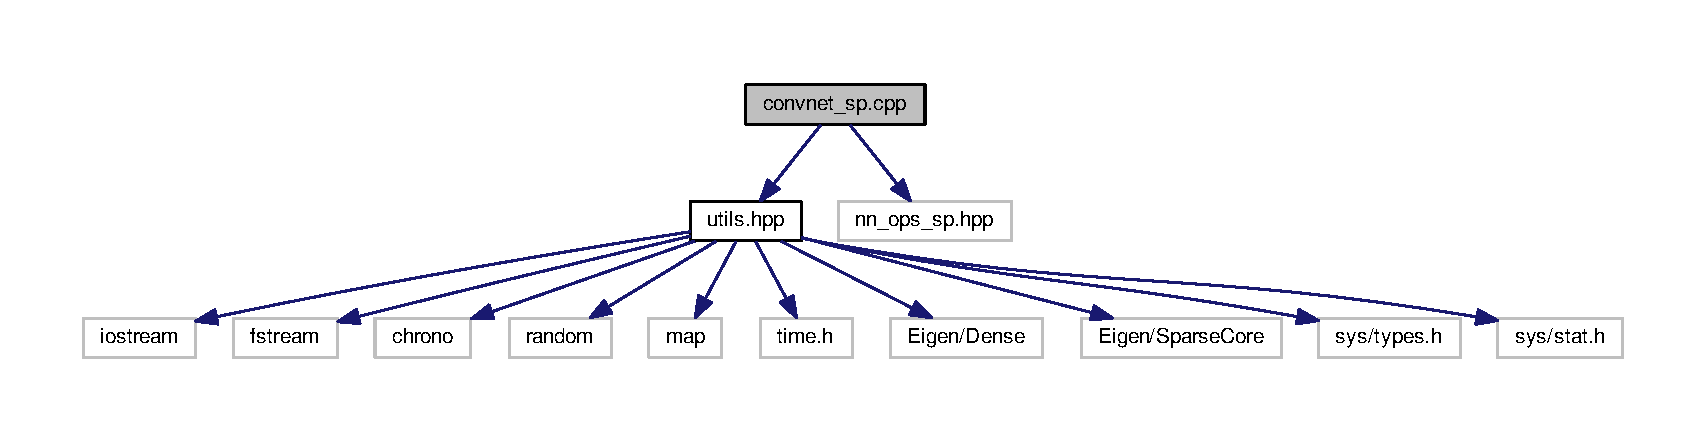
\includegraphics[width=350pt]{convnet__sp_8cpp__incl}
\end{center}
\end{figure}
\subsection*{Functions}
\begin{DoxyCompactItemize}
\item 
\hypertarget{convnet__sp_8cpp_a0ddf1224851353fc92bfbff6f499fa97}{}int {\bfseries main} (int argc, char $\ast$argv\mbox{[}$\,$\mbox{]})\label{convnet__sp_8cpp_a0ddf1224851353fc92bfbff6f499fa97}

\end{DoxyCompactItemize}


\subsection{Detailed Description}
main function for launching experiments with convolutional neural networks and sparse network 

\begin{DoxyAuthor}{Author}
Gaetan Marceau Caron \& Yann Ollivier 
\end{DoxyAuthor}
\begin{DoxyVersion}{Version}
1.\+0 
\end{DoxyVersion}

\hypertarget{nn__ops_8hpp}{}\section{nn\+\_\+ops.\+hpp File Reference}
\label{nn__ops_8hpp}\index{nn\+\_\+ops.\+hpp@{nn\+\_\+ops.\+hpp}}


Implementation of the functions required for neural networks.  


{\ttfamily \#include $<$functional$>$}\\*
{\ttfamily \#include $<$Eigen/\+Dense$>$}\\*
{\ttfamily \#include $<$algorithm$>$}\\*
{\ttfamily \#include $<$assert.\+h$>$}\\*
{\ttfamily \#include $<$limits$>$}\\*
{\ttfamily \#include \char`\"{}utils.\+hpp\char`\"{}}\\*
Include dependency graph for nn\+\_\+ops.\+hpp\+:
\nopagebreak
\begin{figure}[H]
\begin{center}
\leavevmode
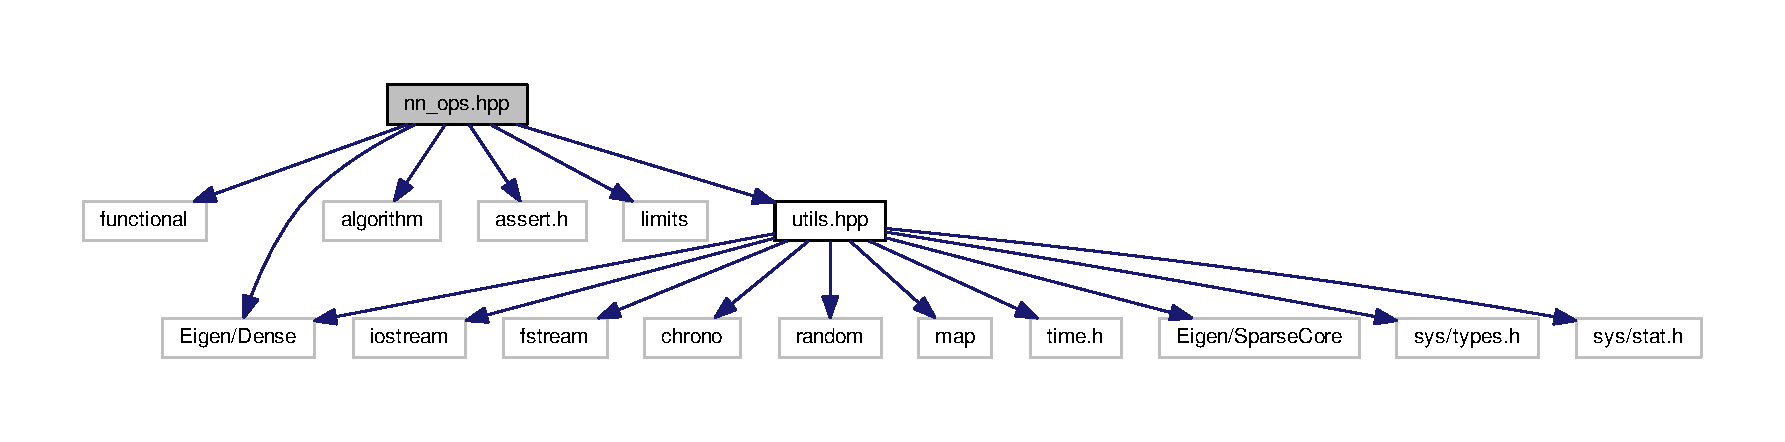
\includegraphics[width=350pt]{nn__ops_8hpp__incl}
\end{center}
\end{figure}
This graph shows which files directly or indirectly include this file\+:
\nopagebreak
\begin{figure}[H]
\begin{center}
\leavevmode
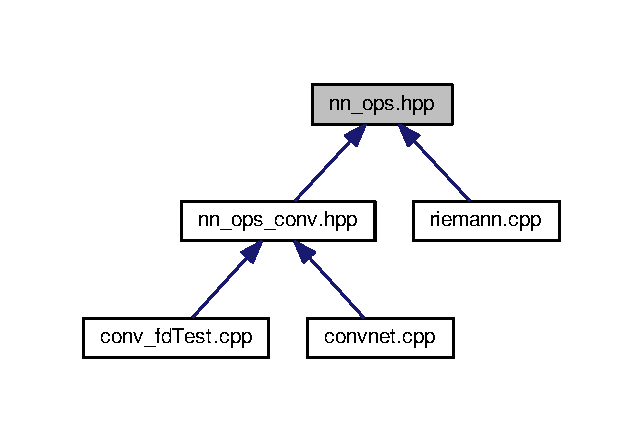
\includegraphics[width=309pt]{nn__ops_8hpp__dep__incl}
\end{center}
\end{figure}
\subsection*{Functions}
\begin{DoxyCompactItemize}
\item 
void \hyperlink{nn__ops_8hpp_a90b8525c0edded9e3420dc56dbb9332f}{init\+Weight} (const unsigned n\+\_\+act0, const unsigned n\+\_\+act1, const double sigma, My\+Matrix \&W)
\begin{DoxyCompactList}\small\item\em Initialize the weights of a layer with a reweighted normal noise. \end{DoxyCompactList}\item 
int \hyperlink{nn__ops_8hpp_a2a07778f5ff97c5d5581276d663ede6e}{init\+Network} (const std\+::vector$<$ unsigned $>$ \&nn\+\_\+arch, const std\+::string act\+\_\+func, std\+::vector$<$ My\+Matrix $>$ \&W, std\+::vector$<$ My\+Vector $>$ \&B)
\begin{DoxyCompactList}\small\item\em Initialize the parameters of the Neural Network computational graph. \end{DoxyCompactList}\item 
double \hyperlink{nn__ops_8hpp_a22f109ce3d23796de9d34fb9eee73040}{sign\+Func} (double x)
\begin{DoxyCompactList}\small\item\em Implementation of the sign function. \end{DoxyCompactList}\item 
double \hyperlink{nn__ops_8hpp_a03a2f1c37574a2bc61630b6e5bf86dcf}{square\+Func} (double x)
\begin{DoxyCompactList}\small\item\em Implementation of the square function. \end{DoxyCompactList}\item 
double \hyperlink{nn__ops_8hpp_a6ceeb10733d64ab2587e136e884c2ec8}{sqrt\+Func} (double x)
\begin{DoxyCompactList}\small\item\em Implementation of the square-\/root function. \end{DoxyCompactList}\item 
double \hyperlink{nn__ops_8hpp_a6bac3899a024aa93b77e99e169f1e86c}{sum\+Cst\+Func} (double x, double cst)
\begin{DoxyCompactList}\small\item\em Implementation of the translation function. \end{DoxyCompactList}\item 
void \hyperlink{nn__ops_8hpp_a4c86f2557fe76d7b0ca7c5111eb7927b}{softmax} (const My\+Matrix \&a, My\+Matrix \&out)
\begin{DoxyCompactList}\small\item\em Implementation of the softmax function Take a matrix (n\+\_\+example X n\+\_\+class) of values and return a matrix (n\+\_\+example X n\+\_\+class) where each line is a probability distribution over the classes. \end{DoxyCompactList}\item 
void \hyperlink{nn__ops_8hpp_a1ee99de11ae8d8f50b32c2037ffd1d1b}{logistic} (const bool deriv\+\_\+flag, const My\+Matrix \&z, My\+Matrix \&a, My\+Matrix \&da)
\begin{DoxyCompactList}\small\item\em Implementation of the logistic function and its derivative. \end{DoxyCompactList}\item 
void \hyperlink{nn__ops_8hpp_aa8e7c94ef2b705a126e52d0ea2fa9901}{my\+\_\+tanh} (const bool deriv\+\_\+flag, const My\+Matrix \&z, My\+Matrix \&a, My\+Matrix \&da)
\begin{DoxyCompactList}\small\item\em Implementation of the tanh function and its derivative. \end{DoxyCompactList}\item 
void \hyperlink{nn__ops_8hpp_af47e86a1783f4c04ee25301f3ec37866}{relu} (const bool deriv\+\_\+flag, const My\+Matrix \&z, My\+Matrix \&a, My\+Matrix \&da)
\begin{DoxyCompactList}\small\item\em Implementation of the rectified linear unit (Re\+L\+U) function and its derivative. \end{DoxyCompactList}\item 
void \hyperlink{nn__ops_8hpp_ac56dfda8be864dadf5db85c56978171d}{dropout} (const double prob, My\+Matrix \&A, My\+Matrix \&B)
\begin{DoxyCompactList}\small\item\em Implementation of the dropout regularization technique. \end{DoxyCompactList}\item 
void \hyperlink{nn__ops_8hpp_afe6393d9948ae9a81cb1292aad353c48}{dropout} (const double prob, My\+Matrix \&A)
\begin{DoxyCompactList}\small\item\em Implementation of the dropout regularization technique. \end{DoxyCompactList}\item 
void \hyperlink{nn__ops_8hpp_a333e03b7cdb8f33e9619edf27f56d6cb}{fprop} (const bool dropout\+\_\+flag, const double dropout\+\_\+prob, const Activation\+Function \&act\+\_\+func, const std\+::vector$<$ My\+Matrix $>$ \&W, const std\+::vector$<$ My\+Vector $>$ \&B, const My\+Matrix \&X\+\_\+batch, std\+::vector$<$ My\+Matrix $>$ \&Z, std\+::vector$<$ My\+Matrix $>$ \&A, std\+::vector$<$ My\+Matrix $>$ \&d\+A)
\begin{DoxyCompactList}\small\item\em Implementation of the forward propagation algorithm. \end{DoxyCompactList}\item 
void \hyperlink{nn__ops_8hpp_a1c7cf6b20b44ba081abe2a5e0110a599}{bprop} (const std\+::vector$<$ My\+Matrix $>$ \&W, const std\+::vector$<$ My\+Matrix $>$ \&d\+A, std\+::vector$<$ My\+Matrix $>$ \&grad\+B)
\begin{DoxyCompactList}\small\item\em Implementation of the backpropagation algorithm. \end{DoxyCompactList}\item 
{\footnotesize template$<$class T $>$ }\\void \hyperlink{nn__ops_8hpp_aaa5dfcccaa4f859b162005465984f40e}{update\+Param} (const double eta, const std\+::string regularizer, const double lambda, const T \&dparams, T \&params)
\begin{DoxyCompactList}\small\item\em Templated function for updating matrices or vectors. \end{DoxyCompactList}\item 
void \hyperlink{nn__ops_8hpp_ac8a4ddb1d085a6e8f288882dc5e2273f}{update} (const double eta, const std\+::vector$<$ My\+Matrix $>$ \&grad\+B, const std\+::vector$<$ My\+Matrix $>$ \&A, const My\+Matrix \&X\+\_\+batch, const std\+::string regularizer, const double lambda, std\+::vector$<$ My\+Matrix $>$ \&W, std\+::vector$<$ My\+Vector $>$ \&B)
\begin{DoxyCompactList}\small\item\em Implementation of the update function of the gradient descent algorithm. \end{DoxyCompactList}\item 
void \hyperlink{nn__ops_8hpp_a3c2822a2bbb5ca3701af33bbc402e54f}{adagrad\+Update} (const double eta, const std\+::vector$<$ My\+Matrix $>$ \&grad\+B, const std\+::vector$<$ My\+Matrix $>$ \&A, const My\+Matrix \&X\+\_\+batch, const std\+::string regularizer, const double lambda, const double mat\+\_\+reg, const double autocorr, std\+::vector$<$ My\+Matrix $>$ \&W, std\+::vector$<$ My\+Vector $>$ \&B, std\+::vector$<$ My\+Matrix $>$ \&mu\+\_\+d\+W, std\+::vector$<$ My\+Vector $>$ \&mu\+\_\+d\+B)
\begin{DoxyCompactList}\small\item\em function that performs the adagrad update rule \end{DoxyCompactList}\item 
void \hyperlink{nn__ops_8hpp_a9a994e746ada8c2bd3f11b68114db234}{compute\+Loss} (const Activation\+Function \&act\+\_\+func, const My\+Matrix \&X, const My\+Vector \&Y, const std\+::vector$<$ My\+Matrix $>$ \&W, const std\+::vector$<$ My\+Vector $>$ \&B, double \&loss, double \&accuracy)
\begin{DoxyCompactList}\small\item\em function that compute the Negative Log-\/likelihood and the accuracy of the model \end{DoxyCompactList}\item 
void \hyperlink{nn__ops_8hpp_ad4e3600f69eecf523fb78bb9ffd4ee24}{compute\+Loss} (const Activation\+Function \&act\+\_\+func, const My\+Matrix \&X, const My\+Vector \&Y, const std\+::vector$<$ My\+Matrix $>$ \&W, const std\+::vector$<$ My\+Vector $>$ \&B, const \hyperlink{struct_params}{Params} params, double \&loss, double \&accuracy)
\begin{DoxyCompactList}\small\item\em function that compute the Negative Log-\/likelihood and the accuracy of the model (cannot be used with dropout since the mask will be activated!) \end{DoxyCompactList}\item 
void \hyperlink{nn__ops_8hpp_a99cafbd2955aafe43ad57a88f7f1db5c}{eval\+Model} (const Activation\+Function \&eval\+\_\+act\+\_\+func, const My\+Matrix \&X\+\_\+train, const My\+Matrix \&Y\+\_\+train, const My\+Matrix \&X\+\_\+valid, const My\+Matrix \&Y\+\_\+valid, const \hyperlink{struct_params}{Params} \&params, std\+::vector$<$ My\+Matrix $>$ W\+\_\+eval, std\+::vector$<$ My\+Vector $>$ B, double \&train\+\_\+loss, double \&train\+\_\+accuracy, double \&valid\+\_\+loss, double \&valid\+\_\+accuracy)
\begin{DoxyCompactList}\small\item\em function that evaluate the model on the training dataset and the validation dataset \end{DoxyCompactList}\item 
void \hyperlink{nn__ops_8hpp_ac98a75118cb5c283016ee1d3009e4591}{update\+Stepsize} (const unsigned t, const double init\+\_\+eta, double \&eta)
\begin{DoxyCompactList}\small\item\em simple implementation of a decreasing step-\/size for ensuring convergence \end{DoxyCompactList}\item 
void \hyperlink{nn__ops_8hpp_aa0628205a0dd1fb71743bcea4ff051d5}{build\+Diag\+Metric} (const std\+::vector$<$ My\+Matrix $>$ \&grad\+B\+\_\+sq, const std\+::vector$<$ My\+Matrix $>$ \&A, const My\+Matrix \&X\+\_\+batch, const std\+::vector$<$ My\+Matrix $>$ \&W, const double mat\+\_\+reg, std\+::vector$<$ My\+Matrix $>$ \&Mii, std\+::vector$<$ My\+Vector $>$ \&M00)
\begin{DoxyCompactList}\small\item\em Function that builds a diagonal metric from the gradient w.\+r.\+t. the pre-\/activation. \end{DoxyCompactList}\item 
void \hyperlink{nn__ops_8hpp_a873ca1a30adcb11f4d90563b14139122}{build\+Q\+D\+Metric} (const std\+::vector$<$ My\+Matrix $>$ \&grad\+B\+\_\+sq, const std\+::vector$<$ My\+Matrix $>$ \&A, const My\+Matrix \&X\+\_\+batch, const std\+::vector$<$ My\+Matrix $>$ \&W, const double mat\+\_\+reg, std\+::vector$<$ My\+Matrix $>$ \&Mii, std\+::vector$<$ My\+Matrix $>$ \&M0i, std\+::vector$<$ My\+Vector $>$ \&M00)
\begin{DoxyCompactList}\small\item\em Function that builds a quasi-\/diagonal metric from the gradient w.\+r.\+t. the pre-\/activation. \end{DoxyCompactList}\item 
void \hyperlink{nn__ops_8hpp_a8b089ff4f32d95bcacc9a7cfa7bc1ef6}{update\+Metric} (const bool init\+\_\+flag, const double gamma, std\+::vector$<$ My\+Matrix $>$ \&Mii, std\+::vector$<$ My\+Matrix $>$ \&M0i, std\+::vector$<$ My\+Vector $>$ \&M00, std\+::vector$<$ My\+Matrix $>$ \&p\+Mii, std\+::vector$<$ My\+Matrix $>$ \&p\+M0i, std\+::vector$<$ My\+Vector $>$ \&p\+M00)
\begin{DoxyCompactList}\small\item\em Update the quasi-\/diagonal approximation of the metric with an exponential moving average. \end{DoxyCompactList}\item 
void \hyperlink{nn__ops_8hpp_afc59d7c69fc14a16d2fb47f309f3f63b}{update\+Metric} (const bool init\+\_\+flag, const double gamma, std\+::vector$<$ My\+Matrix $>$ \&Mii, std\+::vector$<$ My\+Vector $>$ \&M00, std\+::vector$<$ My\+Matrix $>$ \&p\+Mii, std\+::vector$<$ My\+Vector $>$ \&p\+M00)
\begin{DoxyCompactList}\small\item\em Update the diagonal approximation of the metric with an exponential moving average. \end{DoxyCompactList}\item 
void \hyperlink{nn__ops_8hpp_a5aaf33307c7448b0ed1991deafc24db1}{qd\+Gradient} (const My\+Matrix \&Mii, const My\+Matrix \&M0i, const My\+Vector \&M00, const My\+Matrix \&d\+W, const My\+Vector \&d\+B, My\+Matrix \&qd\+\_\+d\+W, My\+Vector \&qd\+\_\+d\+B)
\begin{DoxyCompactList}\small\item\em Compute the natural gradient with the quasi-\/diagonal approximation. \end{DoxyCompactList}\item 
void \hyperlink{nn__ops_8hpp_af144ec609311b53a6c4d0cb6678932b9}{diag\+Gradient} (const My\+Matrix \&Mii, const My\+Vector \&M00, const My\+Matrix \&d\+W, const My\+Vector \&d\+B, My\+Matrix \&qd\+\_\+d\+W, My\+Vector \&qd\+\_\+d\+B)
\begin{DoxyCompactList}\small\item\em Compute the natural gradient with the diagonal approximation. \end{DoxyCompactList}\item 
void \hyperlink{nn__ops_8hpp_a5a372ad6a43f1c26470b5125125986ad}{update} (const double eta, const std\+::vector$<$ My\+Matrix $>$ \&grad\+B, const std\+::vector$<$ My\+Matrix $>$ \&A, const My\+Matrix \&X\+\_\+batch, const std\+::string regularizer, const double lambda, std\+::vector$<$ My\+Matrix $>$ \&W, std\+::vector$<$ My\+Vector $>$ \&B, std\+::vector$<$ My\+Matrix $>$ \&Mii, std\+::vector$<$ My\+Matrix $>$ \&M0i, std\+::vector$<$ My\+Vector $>$ \&M00)
\begin{DoxyCompactList}\small\item\em Implementation of the update function of the quasi-\/diagonal natural gradient descent algorithm. \end{DoxyCompactList}\item 
void \hyperlink{nn__ops_8hpp_a2be07c086229dee20135008288130b0c}{update} (const double eta, const std\+::vector$<$ My\+Matrix $>$ \&grad\+B, const std\+::vector$<$ My\+Matrix $>$ \&A, const My\+Matrix \&X\+\_\+batch, const std\+::string regularizer, const double lambda, std\+::vector$<$ My\+Matrix $>$ \&W, std\+::vector$<$ My\+Vector $>$ \&B, std\+::vector$<$ My\+Matrix $>$ \&Mii, std\+::vector$<$ My\+Vector $>$ \&M00)
\begin{DoxyCompactList}\small\item\em Implementation of the update function of the diagonal natural gradient descent algorithm. \end{DoxyCompactList}\item 
void \hyperlink{nn__ops_8hpp_abdf2ed53acfc5b2df65b85c1f5d1970f}{adaptive\+Rule} (const double train\+\_\+loss, double \&prev\+\_\+loss, double \&eta, std\+::vector$<$ My\+Matrix $>$ \&W, std\+::vector$<$ My\+Vector $>$ \&B, std\+::vector$<$ My\+Matrix $>$ \&p\+Mii, std\+::vector$<$ My\+Matrix $>$ \&p\+M0i, std\+::vector$<$ My\+Vector $>$ \&p\+M00, std\+::vector$<$ My\+Matrix $>$ \&p\+W, std\+::vector$<$ My\+Vector $>$ \&p\+B, std\+::vector$<$ My\+Matrix $>$ \&pp\+Mii, std\+::vector$<$ My\+Matrix $>$ \&pp\+M0i, std\+::vector$<$ My\+Vector $>$ \&pp\+M00)
\begin{DoxyCompactList}\small\item\em Implementation of a simple 0.\+5/1.2 step-\/size adaptation rule. \end{DoxyCompactList}\item 
void \hyperlink{nn__ops_8hpp_aa315c58532f165c406aa803c1524a9a8}{qd\+Bpm\+Bprop} (const std\+::vector$<$ My\+Matrix $>$ \&W, const std\+::vector$<$ My\+Matrix $>$ \&d\+A, std\+::vector$<$ My\+Matrix $>$ \&bp\+\_\+grad\+B)
\begin{DoxyCompactList}\small\item\em Implementation of the metric backpropagation algorithm. \end{DoxyCompactList}\item 
void \hyperlink{nn__ops_8hpp_ab5839ec0cc5d7bcbf94b68562f365bee}{compute\+Mc\+Error} (const My\+Matrix \&out, My\+Matrix \&mc\+\_\+error)
\begin{DoxyCompactList}\small\item\em Function that sample a label randomly according to the output distribution and evaluate the gradient w.\+r.\+t. to the output This function is required by the algorithm qd\+M\+C\+Nat. \end{DoxyCompactList}\item 
\hypertarget{nn__ops_8hpp_a098dfb7eceed6e3e86c4866ffd2369d1}{}void {\bfseries init\+Sliding\+Metric} (const std\+::vector$<$ My\+Matrix $>$ \&W, std\+::vector$<$ My\+Matrix $>$ \&p\+Mii, std\+::vector$<$ My\+Matrix $>$ \&p\+M0i, std\+::vector$<$ My\+Vector $>$ \&p\+M00)\label{nn__ops_8hpp_a098dfb7eceed6e3e86c4866ffd2369d1}

\item 
\hypertarget{nn__ops_8hpp_a63eea3fc804396e7f95d93380c997358}{}void {\bfseries compute\+I\+S\+Error} (const My\+Matrix \&out, const My\+Matrix \&one\+\_\+hot\+\_\+batch, const double q, My\+Matrix \&mc\+\_\+error)\label{nn__ops_8hpp_a63eea3fc804396e7f95d93380c997358}

\item 
\hypertarget{nn__ops_8hpp_a41422fe592bc3974f9dbcde6e1422bfa}{}void {\bfseries compute\+Lazy\+Error} (const My\+Matrix \&out, const My\+Matrix \&one\+\_\+hot\+\_\+batch, My\+Matrix \&lazy\+\_\+error)\label{nn__ops_8hpp_a41422fe592bc3974f9dbcde6e1422bfa}

\item 
\hypertarget{nn__ops_8hpp_a4bc298a63450bce97f16047a8be8c0cb}{}void {\bfseries test\+Update} (const double eta, const std\+::vector$<$ My\+Matrix $>$ \&grad\+B, const std\+::vector$<$ My\+Matrix $>$ \&A, const My\+Matrix \&X\+\_\+batch, const std\+::string regularizer, const double lambda, std\+::vector$<$ My\+Matrix $>$ \&W, std\+::vector$<$ My\+Vector $>$ \&B, std\+::vector$<$ My\+Matrix $>$ \&D\+W, std\+::vector$<$ My\+Vector $>$ \&D\+B)\label{nn__ops_8hpp_a4bc298a63450bce97f16047a8be8c0cb}

\item 
\hypertarget{nn__ops_8hpp_a07d054f437b06f4d5a4804fd29874b46}{}void {\bfseries update\+Test} (const double eta, const std\+::vector$<$ My\+Matrix $>$ \&grad\+B, const std\+::vector$<$ My\+Matrix $>$ \&A, const My\+Matrix \&X\+\_\+batch, const std\+::string regularizer, const double lambda, std\+::vector$<$ My\+Matrix $>$ \&W, std\+::vector$<$ My\+Vector $>$ \&B, std\+::vector$<$ My\+Matrix $>$ \&Mii, std\+::vector$<$ My\+Matrix $>$ \&M0i, std\+::vector$<$ My\+Vector $>$ \&M00)\label{nn__ops_8hpp_a07d054f437b06f4d5a4804fd29874b46}

\end{DoxyCompactItemize}


\subsection{Detailed Description}
Implementation of the functions required for neural networks. 

\begin{DoxyAuthor}{Author}
Gaetan Marceau Caron \& Yann Ollivier 
\end{DoxyAuthor}
\begin{DoxyVersion}{Version}
1.\+0 
\end{DoxyVersion}


\subsection{Function Documentation}
\hypertarget{nn__ops_8hpp_a3c2822a2bbb5ca3701af33bbc402e54f}{}\index{nn\+\_\+ops.\+hpp@{nn\+\_\+ops.\+hpp}!adagrad\+Update@{adagrad\+Update}}
\index{adagrad\+Update@{adagrad\+Update}!nn\+\_\+ops.\+hpp@{nn\+\_\+ops.\+hpp}}
\subsubsection[{adagrad\+Update}]{\setlength{\rightskip}{0pt plus 5cm}void adagrad\+Update (
\begin{DoxyParamCaption}
\item[{const double}]{eta, }
\item[{const std\+::vector$<$ My\+Matrix $>$ \&}]{grad\+B, }
\item[{const std\+::vector$<$ My\+Matrix $>$ \&}]{A, }
\item[{const My\+Matrix \&}]{X\+\_\+batch, }
\item[{const std\+::string}]{regularizer, }
\item[{const double}]{lambda, }
\item[{const double}]{mat\+\_\+reg, }
\item[{const double}]{autocorr, }
\item[{std\+::vector$<$ My\+Matrix $>$ \&}]{W, }
\item[{std\+::vector$<$ My\+Vector $>$ \&}]{B, }
\item[{std\+::vector$<$ My\+Matrix $>$ \&}]{mu\+\_\+d\+W, }
\item[{std\+::vector$<$ My\+Vector $>$ \&}]{mu\+\_\+d\+B}
\end{DoxyParamCaption}
)}\label{nn__ops_8hpp_a3c2822a2bbb5ca3701af33bbc402e54f}


function that performs the adagrad update rule 


\begin{DoxyParams}{Parameters}
{\em eta} & the gradient descent step-\/size \\
\hline
{\em grad\+B} & a standard vector of the gradient w.\+r.\+t. the pre-\/activation values (one per layer) \\
\hline
{\em A} & a standard vector of activation values (one per layer) \\
\hline
{\em X\+\_\+batch} & a matrix containing the training examples of the current minibatch \\
\hline
{\em regularizer} & the string of the norm regularizer (L1 or L2) \\
\hline
{\em lambda} & the amplitude of the regularization term \\
\hline
{\em mat\+\_\+reg} & a numerical regularization term s.\+t. there is no division by zero \\
\hline
{\em autocorr} & the autocorrelation coefficient of the adagrad update rule \\
\hline
{\em W} & a standard vector of weight matrices (one per layer) \\
\hline
{\em B} & a standard vector of bias vectors (one per layer) \\
\hline
{\em mu\+\_\+d\+W} & a standard vector of the rolling averages of the weight matrices (one per layer) \\
\hline
{\em mu\+\_\+d\+B} & a standard vector of the rolling averages of the bias vectors (one per layer) \\
\hline
\end{DoxyParams}
\hypertarget{nn__ops_8hpp_abdf2ed53acfc5b2df65b85c1f5d1970f}{}\index{nn\+\_\+ops.\+hpp@{nn\+\_\+ops.\+hpp}!adaptive\+Rule@{adaptive\+Rule}}
\index{adaptive\+Rule@{adaptive\+Rule}!nn\+\_\+ops.\+hpp@{nn\+\_\+ops.\+hpp}}
\subsubsection[{adaptive\+Rule}]{\setlength{\rightskip}{0pt plus 5cm}void adaptive\+Rule (
\begin{DoxyParamCaption}
\item[{const double}]{train\+\_\+loss, }
\item[{double \&}]{prev\+\_\+loss, }
\item[{double \&}]{eta, }
\item[{std\+::vector$<$ My\+Matrix $>$ \&}]{W, }
\item[{std\+::vector$<$ My\+Vector $>$ \&}]{B, }
\item[{std\+::vector$<$ My\+Matrix $>$ \&}]{p\+Mii, }
\item[{std\+::vector$<$ My\+Matrix $>$ \&}]{p\+M0i, }
\item[{std\+::vector$<$ My\+Vector $>$ \&}]{p\+M00, }
\item[{std\+::vector$<$ My\+Matrix $>$ \&}]{p\+W, }
\item[{std\+::vector$<$ My\+Vector $>$ \&}]{p\+B, }
\item[{std\+::vector$<$ My\+Matrix $>$ \&}]{pp\+Mii, }
\item[{std\+::vector$<$ My\+Matrix $>$ \&}]{pp\+M0i, }
\item[{std\+::vector$<$ My\+Vector $>$ \&}]{pp\+M00}
\end{DoxyParamCaption}
)}\label{nn__ops_8hpp_abdf2ed53acfc5b2df65b85c1f5d1970f}


Implementation of a simple 0.\+5/1.2 step-\/size adaptation rule. 


\begin{DoxyParams}{Parameters}
{\em train\+\_\+loss} & the negative log-\/likelihood associated to the current parameters \\
\hline
{\em prev\+\_\+loss} & the negative log-\/likelihood associated to the previous parameters \\
\hline
{\em eta} & the current step-\/size \\
\hline
{\em W} & a standard vector of weight matrices (one per layer) \\
\hline
{\em B} & a standard vector of bias vectors (one per layer) \\
\hline
{\em p\+Mii} & a standard vector of the exponential moving average of Mii \\
\hline
{\em p\+Mi0} & a standard vector of the exponential moving average of M0i \\
\hline
{\em p\+M00} & a standard vector of the exponential moving average of M00 \\
\hline
{\em p\+W} & a standard vector of weight matrices of the previous iteration (one per layer) \\
\hline
{\em p\+B} & a standard vector of bias vectors of the previous iteration (one per layer) \\
\hline
{\em pp\+Mii} & a standard vector of the exponential moving average of Mii of the previous iteration \\
\hline
{\em pp\+Mi0} & a standard vector of the exponential moving average of M0i of the previous iteration \\
\hline
{\em pp\+M00} & a standard vector of the exponential moving average of M00 of the previous iteration \\
\hline
\end{DoxyParams}
\hypertarget{nn__ops_8hpp_a1c7cf6b20b44ba081abe2a5e0110a599}{}\index{nn\+\_\+ops.\+hpp@{nn\+\_\+ops.\+hpp}!bprop@{bprop}}
\index{bprop@{bprop}!nn\+\_\+ops.\+hpp@{nn\+\_\+ops.\+hpp}}
\subsubsection[{bprop}]{\setlength{\rightskip}{0pt plus 5cm}void bprop (
\begin{DoxyParamCaption}
\item[{const std\+::vector$<$ My\+Matrix $>$ \&}]{W, }
\item[{const std\+::vector$<$ My\+Matrix $>$ \&}]{d\+A, }
\item[{std\+::vector$<$ My\+Matrix $>$ \&}]{grad\+B}
\end{DoxyParamCaption}
)}\label{nn__ops_8hpp_a1c7cf6b20b44ba081abe2a5e0110a599}


Implementation of the backpropagation algorithm. 


\begin{DoxyParams}{Parameters}
{\em W} & a standard vector of weight matrices (one per layer) \\
\hline
{\em d\+A} & a standard vector of the derivatives of the activation values (one per layer) \\
\hline
{\em grad\+B} & a standard vector of the gradient w.\+r.\+t. the pre-\/activation values (one per layer) \\
\hline
\end{DoxyParams}
\hypertarget{nn__ops_8hpp_aa0628205a0dd1fb71743bcea4ff051d5}{}\index{nn\+\_\+ops.\+hpp@{nn\+\_\+ops.\+hpp}!build\+Diag\+Metric@{build\+Diag\+Metric}}
\index{build\+Diag\+Metric@{build\+Diag\+Metric}!nn\+\_\+ops.\+hpp@{nn\+\_\+ops.\+hpp}}
\subsubsection[{build\+Diag\+Metric}]{\setlength{\rightskip}{0pt plus 5cm}void build\+Diag\+Metric (
\begin{DoxyParamCaption}
\item[{const std\+::vector$<$ My\+Matrix $>$ \&}]{grad\+B\+\_\+sq, }
\item[{const std\+::vector$<$ My\+Matrix $>$ \&}]{A, }
\item[{const My\+Matrix \&}]{X\+\_\+batch, }
\item[{const std\+::vector$<$ My\+Matrix $>$ \&}]{W, }
\item[{const double}]{mat\+\_\+reg, }
\item[{std\+::vector$<$ My\+Matrix $>$ \&}]{Mii, }
\item[{std\+::vector$<$ My\+Vector $>$ \&}]{M00}
\end{DoxyParamCaption}
)}\label{nn__ops_8hpp_aa0628205a0dd1fb71743bcea4ff051d5}


Function that builds a diagonal metric from the gradient w.\+r.\+t. the pre-\/activation. 


\begin{DoxyParams}{Parameters}
{\em grad\+B\+\_\+sq} & a standard vector of the square of the gradient w.\+r.\+t. the pre-\/activation values (one per layer) \\
\hline
{\em A} & a standard vector of activation values (one per layer) \\
\hline
{\em X\+\_\+batch} & a matrix containing the training examples of the current minibatch \\
\hline
{\em W} & a standard vector of weight matrices (one per layer) \\
\hline
{\em mat\+\_\+reg} & a numerical regularization term s.\+t. the metric is invertible \\
\hline
{\em Mii} & a standard vector of the diagonals of the block sub-\/matrices of the Riemannian metric (one per layer) \\
\hline
{\em M00} & a standard vector of the bias of the block sub-\/matrices of the Riemannian metric (one per layer) \\
\hline
\end{DoxyParams}
\hypertarget{nn__ops_8hpp_a873ca1a30adcb11f4d90563b14139122}{}\index{nn\+\_\+ops.\+hpp@{nn\+\_\+ops.\+hpp}!build\+Q\+D\+Metric@{build\+Q\+D\+Metric}}
\index{build\+Q\+D\+Metric@{build\+Q\+D\+Metric}!nn\+\_\+ops.\+hpp@{nn\+\_\+ops.\+hpp}}
\subsubsection[{build\+Q\+D\+Metric}]{\setlength{\rightskip}{0pt plus 5cm}void build\+Q\+D\+Metric (
\begin{DoxyParamCaption}
\item[{const std\+::vector$<$ My\+Matrix $>$ \&}]{grad\+B\+\_\+sq, }
\item[{const std\+::vector$<$ My\+Matrix $>$ \&}]{A, }
\item[{const My\+Matrix \&}]{X\+\_\+batch, }
\item[{const std\+::vector$<$ My\+Matrix $>$ \&}]{W, }
\item[{const double}]{mat\+\_\+reg, }
\item[{std\+::vector$<$ My\+Matrix $>$ \&}]{Mii, }
\item[{std\+::vector$<$ My\+Matrix $>$ \&}]{M0i, }
\item[{std\+::vector$<$ My\+Vector $>$ \&}]{M00}
\end{DoxyParamCaption}
)}\label{nn__ops_8hpp_a873ca1a30adcb11f4d90563b14139122}


Function that builds a quasi-\/diagonal metric from the gradient w.\+r.\+t. the pre-\/activation. 


\begin{DoxyParams}{Parameters}
{\em grad\+B\+\_\+sq} & a standard vector of the square of the gradient w.\+r.\+t. the pre-\/activation values (one per layer) \\
\hline
{\em A} & a standard vector of activation values (one per layer) \\
\hline
{\em X\+\_\+batch} & a matrix containing the training examples of the current minibatch \\
\hline
{\em W} & a standard vector of weight matrices (one per layer) \\
\hline
{\em mat\+\_\+reg} & a numerical regularization term s.\+t. the metric is invertible \\
\hline
{\em Mii} & a standard vector of the diagonals of the block sub-\/matrices of the Riemannian metric (one per layer) \\
\hline
{\em Mi0} & a standard vector of the weights time the bias (first line) of the block sub-\/matrices of the Riemannian metric (one per layer) \\
\hline
{\em M00} & a standard vector of the bias of the block sub-\/matrices of the Riemannian metric (one per layer) \\
\hline
\end{DoxyParams}
\hypertarget{nn__ops_8hpp_a9a994e746ada8c2bd3f11b68114db234}{}\index{nn\+\_\+ops.\+hpp@{nn\+\_\+ops.\+hpp}!compute\+Loss@{compute\+Loss}}
\index{compute\+Loss@{compute\+Loss}!nn\+\_\+ops.\+hpp@{nn\+\_\+ops.\+hpp}}
\subsubsection[{compute\+Loss}]{\setlength{\rightskip}{0pt plus 5cm}void compute\+Loss (
\begin{DoxyParamCaption}
\item[{const Activation\+Function \&}]{act\+\_\+func, }
\item[{const My\+Matrix \&}]{X, }
\item[{const My\+Vector \&}]{Y, }
\item[{const std\+::vector$<$ My\+Matrix $>$ \&}]{W, }
\item[{const std\+::vector$<$ My\+Vector $>$ \&}]{B, }
\item[{double \&}]{loss, }
\item[{double \&}]{accuracy}
\end{DoxyParamCaption}
)}\label{nn__ops_8hpp_a9a994e746ada8c2bd3f11b68114db234}


function that compute the Negative Log-\/likelihood and the accuracy of the model 


\begin{DoxyParams}{Parameters}
{\em act\+\_\+func} & the reference of the activation function \\
\hline
{\em X} & a matrix containing the training examples \\
\hline
{\em Y} & a vector containing the labels of the examples \\
\hline
{\em W} & a standard vector of weight matrices (one per layer) \\
\hline
{\em B} & a standard vector of bias vectors (one per layer) \\
\hline
{\em loss} & the negative log-\/likelihood \\
\hline
{\em accuracy} & the accuracy \\
\hline
\end{DoxyParams}
\hypertarget{nn__ops_8hpp_ad4e3600f69eecf523fb78bb9ffd4ee24}{}\index{nn\+\_\+ops.\+hpp@{nn\+\_\+ops.\+hpp}!compute\+Loss@{compute\+Loss}}
\index{compute\+Loss@{compute\+Loss}!nn\+\_\+ops.\+hpp@{nn\+\_\+ops.\+hpp}}
\subsubsection[{compute\+Loss}]{\setlength{\rightskip}{0pt plus 5cm}void compute\+Loss (
\begin{DoxyParamCaption}
\item[{const Activation\+Function \&}]{act\+\_\+func, }
\item[{const My\+Matrix \&}]{X, }
\item[{const My\+Vector \&}]{Y, }
\item[{const std\+::vector$<$ My\+Matrix $>$ \&}]{W, }
\item[{const std\+::vector$<$ My\+Vector $>$ \&}]{B, }
\item[{const {\bf Params}}]{params, }
\item[{double \&}]{loss, }
\item[{double \&}]{accuracy}
\end{DoxyParamCaption}
)}\label{nn__ops_8hpp_ad4e3600f69eecf523fb78bb9ffd4ee24}


function that compute the Negative Log-\/likelihood and the accuracy of the model (cannot be used with dropout since the mask will be activated!) 


\begin{DoxyParams}{Parameters}
{\em act\+\_\+func} & the reference of the activation function \\
\hline
{\em X} & a matrix containing the training examples \\
\hline
{\em Y} & a vector containing the labels of the examples \\
\hline
{\em W} & a standard vector of weight matrices (one per layer) \\
\hline
{\em B} & a standard vector of bias vectors (one per layer) \\
\hline
{\em params} & the parameters of the program \\
\hline
{\em loss} & the negative log-\/likelihood \\
\hline
{\em accuracy} & the accuracy \\
\hline
\end{DoxyParams}
\hypertarget{nn__ops_8hpp_ab5839ec0cc5d7bcbf94b68562f365bee}{}\index{nn\+\_\+ops.\+hpp@{nn\+\_\+ops.\+hpp}!compute\+Mc\+Error@{compute\+Mc\+Error}}
\index{compute\+Mc\+Error@{compute\+Mc\+Error}!nn\+\_\+ops.\+hpp@{nn\+\_\+ops.\+hpp}}
\subsubsection[{compute\+Mc\+Error}]{\setlength{\rightskip}{0pt plus 5cm}void compute\+Mc\+Error (
\begin{DoxyParamCaption}
\item[{const My\+Matrix \&}]{out, }
\item[{My\+Matrix \&}]{mc\+\_\+error}
\end{DoxyParamCaption}
)}\label{nn__ops_8hpp_ab5839ec0cc5d7bcbf94b68562f365bee}


Function that sample a label randomly according to the output distribution and evaluate the gradient w.\+r.\+t. to the output This function is required by the algorithm qd\+M\+C\+Nat. 


\begin{DoxyParams}{Parameters}
{\em out} & the probability distribution over the output (values returned by softmax) \\
\hline
{\em mc\+\_\+error} & the gradient w.\+r.\+t. to the output \\
\hline
\end{DoxyParams}
\hypertarget{nn__ops_8hpp_af144ec609311b53a6c4d0cb6678932b9}{}\index{nn\+\_\+ops.\+hpp@{nn\+\_\+ops.\+hpp}!diag\+Gradient@{diag\+Gradient}}
\index{diag\+Gradient@{diag\+Gradient}!nn\+\_\+ops.\+hpp@{nn\+\_\+ops.\+hpp}}
\subsubsection[{diag\+Gradient}]{\setlength{\rightskip}{0pt plus 5cm}void diag\+Gradient (
\begin{DoxyParamCaption}
\item[{const My\+Matrix \&}]{Mii, }
\item[{const My\+Vector \&}]{M00, }
\item[{const My\+Matrix \&}]{d\+W, }
\item[{const My\+Vector \&}]{d\+B, }
\item[{My\+Matrix \&}]{qd\+\_\+d\+W, }
\item[{My\+Vector \&}]{qd\+\_\+d\+B}
\end{DoxyParamCaption}
)}\label{nn__ops_8hpp_af144ec609311b53a6c4d0cb6678932b9}


Compute the natural gradient with the diagonal approximation. 


\begin{DoxyParams}{Parameters}
{\em Mii} & the diagonals of the block sub-\/matrices of the Riemannian metric (one per layer) \\
\hline
{\em M00} & the bias of the block sub-\/matrices of the Riemannian metric (one per layer) \\
\hline
{\em d\+W} & the gradient w.\+r.\+t. the weights \\
\hline
{\em d\+B} & the gradient w.\+r.\+t. the bias \\
\hline
{\em qd\+\_\+d\+W} & the quasi-\/diagonal natural gradient w.\+r.\+t. the weights \\
\hline
{\em qd\+\_\+d\+B} & the quasi-\/diagonal natural gradient w.\+r.\+t. the bias \\
\hline
\end{DoxyParams}
\hypertarget{nn__ops_8hpp_ac56dfda8be864dadf5db85c56978171d}{}\index{nn\+\_\+ops.\+hpp@{nn\+\_\+ops.\+hpp}!dropout@{dropout}}
\index{dropout@{dropout}!nn\+\_\+ops.\+hpp@{nn\+\_\+ops.\+hpp}}
\subsubsection[{dropout}]{\setlength{\rightskip}{0pt plus 5cm}void dropout (
\begin{DoxyParamCaption}
\item[{const double}]{prob, }
\item[{My\+Matrix \&}]{A, }
\item[{My\+Matrix \&}]{B}
\end{DoxyParamCaption}
)}\label{nn__ops_8hpp_ac56dfda8be864dadf5db85c56978171d}


Implementation of the dropout regularization technique. 


\begin{DoxyParams}{Parameters}
{\em prob} & the probability of dropout \\
\hline
{\em A} & a matrix to regularize (n\+\_\+example X n\+\_\+unit) \\
\hline
{\em B} & another matrix to regularize with the same mask (n\+\_\+example X n\+\_\+unit) \\
\hline
\end{DoxyParams}
\hypertarget{nn__ops_8hpp_afe6393d9948ae9a81cb1292aad353c48}{}\index{nn\+\_\+ops.\+hpp@{nn\+\_\+ops.\+hpp}!dropout@{dropout}}
\index{dropout@{dropout}!nn\+\_\+ops.\+hpp@{nn\+\_\+ops.\+hpp}}
\subsubsection[{dropout}]{\setlength{\rightskip}{0pt plus 5cm}void dropout (
\begin{DoxyParamCaption}
\item[{const double}]{prob, }
\item[{My\+Matrix \&}]{A}
\end{DoxyParamCaption}
)}\label{nn__ops_8hpp_afe6393d9948ae9a81cb1292aad353c48}


Implementation of the dropout regularization technique. 


\begin{DoxyParams}{Parameters}
{\em prob} & the probability of dropout \\
\hline
{\em A} & a matrix to regularize (n\+\_\+example X n\+\_\+unit) \\
\hline
\end{DoxyParams}
\hypertarget{nn__ops_8hpp_a99cafbd2955aafe43ad57a88f7f1db5c}{}\index{nn\+\_\+ops.\+hpp@{nn\+\_\+ops.\+hpp}!eval\+Model@{eval\+Model}}
\index{eval\+Model@{eval\+Model}!nn\+\_\+ops.\+hpp@{nn\+\_\+ops.\+hpp}}
\subsubsection[{eval\+Model}]{\setlength{\rightskip}{0pt plus 5cm}void eval\+Model (
\begin{DoxyParamCaption}
\item[{const Activation\+Function \&}]{eval\+\_\+act\+\_\+func, }
\item[{const My\+Matrix \&}]{X\+\_\+train, }
\item[{const My\+Matrix \&}]{Y\+\_\+train, }
\item[{const My\+Matrix \&}]{X\+\_\+valid, }
\item[{const My\+Matrix \&}]{Y\+\_\+valid, }
\item[{const {\bf Params} \&}]{params, }
\item[{std\+::vector$<$ My\+Matrix $>$}]{W\+\_\+eval, }
\item[{std\+::vector$<$ My\+Vector $>$}]{B, }
\item[{double \&}]{train\+\_\+loss, }
\item[{double \&}]{train\+\_\+accuracy, }
\item[{double \&}]{valid\+\_\+loss, }
\item[{double \&}]{valid\+\_\+accuracy}
\end{DoxyParamCaption}
)}\label{nn__ops_8hpp_a99cafbd2955aafe43ad57a88f7f1db5c}


function that evaluate the model on the training dataset and the validation dataset 


\begin{DoxyParams}{Parameters}
{\em eval\+\_\+act\+\_\+func} & the reference of the activation function \\
\hline
{\em X\+\_\+train} & a matrix containing the training examples \\
\hline
{\em Y\+\_\+train} & a vector containing the labels of the training examples \\
\hline
{\em X\+\_\+valid} & a matrix containing the validation examples \\
\hline
{\em Y\+\_\+valid} & a vector containing the labels of the validation examples \\
\hline
{\em params} & the parameters of the program \\
\hline
{\em W\+\_\+eval} & a copy of the standard vector of weight matrices (one per layer) \\
\hline
{\em B} & a standard vector of bias vectors (one per layer) \\
\hline
{\em train\+\_\+loss} & the negative log-\/likelihood on the training set \\
\hline
{\em train\+\_\+accuracy} & the accuracy on the training set \\
\hline
{\em valid\+\_\+loss} & the negative log-\/likelihood on the validation set \\
\hline
{\em valid\+\_\+accuracy} & the accuracy on the validation set \\
\hline
\end{DoxyParams}
\hypertarget{nn__ops_8hpp_a333e03b7cdb8f33e9619edf27f56d6cb}{}\index{nn\+\_\+ops.\+hpp@{nn\+\_\+ops.\+hpp}!fprop@{fprop}}
\index{fprop@{fprop}!nn\+\_\+ops.\+hpp@{nn\+\_\+ops.\+hpp}}
\subsubsection[{fprop}]{\setlength{\rightskip}{0pt plus 5cm}void fprop (
\begin{DoxyParamCaption}
\item[{const bool}]{dropout\+\_\+flag, }
\item[{const double}]{dropout\+\_\+prob, }
\item[{const Activation\+Function \&}]{act\+\_\+func, }
\item[{const std\+::vector$<$ My\+Matrix $>$ \&}]{W, }
\item[{const std\+::vector$<$ My\+Vector $>$ \&}]{B, }
\item[{const My\+Matrix \&}]{X\+\_\+batch, }
\item[{std\+::vector$<$ My\+Matrix $>$ \&}]{Z, }
\item[{std\+::vector$<$ My\+Matrix $>$ \&}]{A, }
\item[{std\+::vector$<$ My\+Matrix $>$ \&}]{d\+A}
\end{DoxyParamCaption}
)}\label{nn__ops_8hpp_a333e03b7cdb8f33e9619edf27f56d6cb}


Implementation of the forward propagation algorithm. 


\begin{DoxyParams}{Parameters}
{\em dropout\+\_\+flag} & the flag for activating dropout regularization \\
\hline
{\em dropout\+\_\+prob} & the probability of dropout (dropout\+\_\+flag must be true) \\
\hline
{\em act\+\_\+func} & the reference of the activation function \\
\hline
{\em W} & a standard vector of weight matrices (one per layer) \\
\hline
{\em B} & a standard vector of bias vectors (one per layer) \\
\hline
{\em X\+\_\+batch} & a matrix containing the training examples of the current minibatch \\
\hline
{\em Z} & a standard vector of pre-\/activation values (one per layer) \\
\hline
{\em A} & a standard vector of activation values (one per layer) \\
\hline
{\em d\+A} & a standard vector of the derivatives of the activation values (one per layer) \\
\hline
\end{DoxyParams}
\hypertarget{nn__ops_8hpp_a2a07778f5ff97c5d5581276d663ede6e}{}\index{nn\+\_\+ops.\+hpp@{nn\+\_\+ops.\+hpp}!init\+Network@{init\+Network}}
\index{init\+Network@{init\+Network}!nn\+\_\+ops.\+hpp@{nn\+\_\+ops.\+hpp}}
\subsubsection[{init\+Network}]{\setlength{\rightskip}{0pt plus 5cm}int init\+Network (
\begin{DoxyParamCaption}
\item[{const std\+::vector$<$ unsigned $>$ \&}]{nn\+\_\+arch, }
\item[{const std\+::string}]{act\+\_\+func, }
\item[{std\+::vector$<$ My\+Matrix $>$ \&}]{W, }
\item[{std\+::vector$<$ My\+Vector $>$ \&}]{B}
\end{DoxyParamCaption}
)}\label{nn__ops_8hpp_a2a07778f5ff97c5d5581276d663ede6e}


Initialize the parameters of the Neural Network computational graph. 


\begin{DoxyParams}{Parameters}
{\em nn\+\_\+arch} & number of activation units for each layer \\
\hline
{\em act\+\_\+func} & string representing the activation function \\
\hline
{\em W} & a standard vector of weight matrices (one per layer) \\
\hline
{\em B} & a standard vector of bias vectors (one per layer) \\
\hline
\end{DoxyParams}
\begin{DoxyReturn}{Returns}
the number of parameters 
\end{DoxyReturn}
\hypertarget{nn__ops_8hpp_a90b8525c0edded9e3420dc56dbb9332f}{}\index{nn\+\_\+ops.\+hpp@{nn\+\_\+ops.\+hpp}!init\+Weight@{init\+Weight}}
\index{init\+Weight@{init\+Weight}!nn\+\_\+ops.\+hpp@{nn\+\_\+ops.\+hpp}}
\subsubsection[{init\+Weight}]{\setlength{\rightskip}{0pt plus 5cm}void init\+Weight (
\begin{DoxyParamCaption}
\item[{const unsigned}]{n\+\_\+act0, }
\item[{const unsigned}]{n\+\_\+act1, }
\item[{const double}]{sigma, }
\item[{My\+Matrix \&}]{W}
\end{DoxyParamCaption}
)}\label{nn__ops_8hpp_a90b8525c0edded9e3420dc56dbb9332f}


Initialize the weights of a layer with a reweighted normal noise. 


\begin{DoxyParams}{Parameters}
{\em n\+\_\+act0} & number of input units \\
\hline
{\em n\+\_\+act1} & number of output units \\
\hline
{\em sigma} & stddev of the normal noise \\
\hline
{\em W} & weight matrix returned by the function \\
\hline
\end{DoxyParams}
\hypertarget{nn__ops_8hpp_a1ee99de11ae8d8f50b32c2037ffd1d1b}{}\index{nn\+\_\+ops.\+hpp@{nn\+\_\+ops.\+hpp}!logistic@{logistic}}
\index{logistic@{logistic}!nn\+\_\+ops.\+hpp@{nn\+\_\+ops.\+hpp}}
\subsubsection[{logistic}]{\setlength{\rightskip}{0pt plus 5cm}void logistic (
\begin{DoxyParamCaption}
\item[{const bool}]{deriv\+\_\+flag, }
\item[{const My\+Matrix \&}]{z, }
\item[{My\+Matrix \&}]{a, }
\item[{My\+Matrix \&}]{da}
\end{DoxyParamCaption}
)}\label{nn__ops_8hpp_a1ee99de11ae8d8f50b32c2037ffd1d1b}


Implementation of the logistic function and its derivative. 


\begin{DoxyParams}{Parameters}
{\em deriv\+\_\+flag} & a flag for computing the derivative at the same time \\
\hline
{\em z} & the pre-\/activation matrix (n\+\_\+example X n\+\_\+unit) \\
\hline
{\em a} & the activation matrix (n\+\_\+example X n\+\_\+unit) \\
\hline
{\em da} & the derivative activation matrix (n\+\_\+example X n\+\_\+unit) \\
\hline
\end{DoxyParams}
\hypertarget{nn__ops_8hpp_aa8e7c94ef2b705a126e52d0ea2fa9901}{}\index{nn\+\_\+ops.\+hpp@{nn\+\_\+ops.\+hpp}!my\+\_\+tanh@{my\+\_\+tanh}}
\index{my\+\_\+tanh@{my\+\_\+tanh}!nn\+\_\+ops.\+hpp@{nn\+\_\+ops.\+hpp}}
\subsubsection[{my\+\_\+tanh}]{\setlength{\rightskip}{0pt plus 5cm}void my\+\_\+tanh (
\begin{DoxyParamCaption}
\item[{const bool}]{deriv\+\_\+flag, }
\item[{const My\+Matrix \&}]{z, }
\item[{My\+Matrix \&}]{a, }
\item[{My\+Matrix \&}]{da}
\end{DoxyParamCaption}
)}\label{nn__ops_8hpp_aa8e7c94ef2b705a126e52d0ea2fa9901}


Implementation of the tanh function and its derivative. 


\begin{DoxyParams}{Parameters}
{\em deriv\+\_\+flag} & a flag for computing the derivative at the same time \\
\hline
{\em z} & the pre-\/activation matrix (n\+\_\+example X n\+\_\+unit) \\
\hline
{\em a} & the activation matrix (n\+\_\+example X n\+\_\+unit) \\
\hline
{\em da} & the derivative activation matrix (n\+\_\+example X n\+\_\+unit) \\
\hline
\end{DoxyParams}
\hypertarget{nn__ops_8hpp_aa315c58532f165c406aa803c1524a9a8}{}\index{nn\+\_\+ops.\+hpp@{nn\+\_\+ops.\+hpp}!qd\+Bpm\+Bprop@{qd\+Bpm\+Bprop}}
\index{qd\+Bpm\+Bprop@{qd\+Bpm\+Bprop}!nn\+\_\+ops.\+hpp@{nn\+\_\+ops.\+hpp}}
\subsubsection[{qd\+Bpm\+Bprop}]{\setlength{\rightskip}{0pt plus 5cm}void qd\+Bpm\+Bprop (
\begin{DoxyParamCaption}
\item[{const std\+::vector$<$ My\+Matrix $>$ \&}]{W, }
\item[{const std\+::vector$<$ My\+Matrix $>$ \&}]{d\+A, }
\item[{std\+::vector$<$ My\+Matrix $>$ \&}]{bp\+\_\+grad\+B}
\end{DoxyParamCaption}
)}\label{nn__ops_8hpp_aa315c58532f165c406aa803c1524a9a8}


Implementation of the metric backpropagation algorithm. 


\begin{DoxyParams}{Parameters}
{\em W} & a standard vector of weight matrices (one per layer) \\
\hline
{\em d\+A} & a standard vector of the derivatives of the activation values (one per layer) \\
\hline
{\em bp\+\_\+grad\+B} & a standard vector of the backpropagated metric (one per layer) \\
\hline
\end{DoxyParams}
\hypertarget{nn__ops_8hpp_a5aaf33307c7448b0ed1991deafc24db1}{}\index{nn\+\_\+ops.\+hpp@{nn\+\_\+ops.\+hpp}!qd\+Gradient@{qd\+Gradient}}
\index{qd\+Gradient@{qd\+Gradient}!nn\+\_\+ops.\+hpp@{nn\+\_\+ops.\+hpp}}
\subsubsection[{qd\+Gradient}]{\setlength{\rightskip}{0pt plus 5cm}void qd\+Gradient (
\begin{DoxyParamCaption}
\item[{const My\+Matrix \&}]{Mii, }
\item[{const My\+Matrix \&}]{M0i, }
\item[{const My\+Vector \&}]{M00, }
\item[{const My\+Matrix \&}]{d\+W, }
\item[{const My\+Vector \&}]{d\+B, }
\item[{My\+Matrix \&}]{qd\+\_\+d\+W, }
\item[{My\+Vector \&}]{qd\+\_\+d\+B}
\end{DoxyParamCaption}
)}\label{nn__ops_8hpp_a5aaf33307c7448b0ed1991deafc24db1}


Compute the natural gradient with the quasi-\/diagonal approximation. 


\begin{DoxyParams}{Parameters}
{\em Mii} & the diagonals of the block sub-\/matrices of the Riemannian metric (one per layer) \\
\hline
{\em Mi0} & the weights time the bias (first line) of the block sub-\/matrices of the Riemannian metric (one per layer) \\
\hline
{\em M00} & the bias of the block sub-\/matrices of the Riemannian metric (one per layer) \\
\hline
{\em d\+W} & the gradient w.\+r.\+t. the weights \\
\hline
{\em d\+B} & the gradient w.\+r.\+t. the bias \\
\hline
{\em qd\+\_\+d\+W} & the quasi-\/diagonal natural gradient w.\+r.\+t. the weights \\
\hline
{\em qd\+\_\+d\+B} & the quasi-\/diagonal natural gradient w.\+r.\+t. the bias \\
\hline
\end{DoxyParams}
\hypertarget{nn__ops_8hpp_af47e86a1783f4c04ee25301f3ec37866}{}\index{nn\+\_\+ops.\+hpp@{nn\+\_\+ops.\+hpp}!relu@{relu}}
\index{relu@{relu}!nn\+\_\+ops.\+hpp@{nn\+\_\+ops.\+hpp}}
\subsubsection[{relu}]{\setlength{\rightskip}{0pt plus 5cm}void relu (
\begin{DoxyParamCaption}
\item[{const bool}]{deriv\+\_\+flag, }
\item[{const My\+Matrix \&}]{z, }
\item[{My\+Matrix \&}]{a, }
\item[{My\+Matrix \&}]{da}
\end{DoxyParamCaption}
)}\label{nn__ops_8hpp_af47e86a1783f4c04ee25301f3ec37866}


Implementation of the rectified linear unit (Re\+L\+U) function and its derivative. 


\begin{DoxyParams}{Parameters}
{\em deriv\+\_\+flag} & a flag for computing the derivative at the same time \\
\hline
{\em z} & the pre-\/activation matrix (n\+\_\+example X n\+\_\+unit) \\
\hline
{\em a} & the activation matrix (n\+\_\+example X n\+\_\+unit) \\
\hline
{\em da} & the derivative activation matrix (n\+\_\+example X n\+\_\+unit) \\
\hline
\end{DoxyParams}
\hypertarget{nn__ops_8hpp_a22f109ce3d23796de9d34fb9eee73040}{}\index{nn\+\_\+ops.\+hpp@{nn\+\_\+ops.\+hpp}!sign\+Func@{sign\+Func}}
\index{sign\+Func@{sign\+Func}!nn\+\_\+ops.\+hpp@{nn\+\_\+ops.\+hpp}}
\subsubsection[{sign\+Func}]{\setlength{\rightskip}{0pt plus 5cm}double sign\+Func (
\begin{DoxyParamCaption}
\item[{double}]{x}
\end{DoxyParamCaption}
)}\label{nn__ops_8hpp_a22f109ce3d23796de9d34fb9eee73040}


Implementation of the sign function. 


\begin{DoxyParams}{Parameters}
{\em x} & an input value \\
\hline
\end{DoxyParams}
\begin{DoxyReturn}{Returns}
the sign of x 
\end{DoxyReturn}
\hypertarget{nn__ops_8hpp_a4c86f2557fe76d7b0ca7c5111eb7927b}{}\index{nn\+\_\+ops.\+hpp@{nn\+\_\+ops.\+hpp}!softmax@{softmax}}
\index{softmax@{softmax}!nn\+\_\+ops.\+hpp@{nn\+\_\+ops.\+hpp}}
\subsubsection[{softmax}]{\setlength{\rightskip}{0pt plus 5cm}void softmax (
\begin{DoxyParamCaption}
\item[{const My\+Matrix \&}]{a, }
\item[{My\+Matrix \&}]{out}
\end{DoxyParamCaption}
)}\label{nn__ops_8hpp_a4c86f2557fe76d7b0ca7c5111eb7927b}


Implementation of the softmax function Take a matrix (n\+\_\+example X n\+\_\+class) of values and return a matrix (n\+\_\+example X n\+\_\+class) where each line is a probability distribution over the classes. 


\begin{DoxyParams}{Parameters}
{\em a} & the pre-\/activation values \\
\hline
{\em out} & the probability distribution \\
\hline
\end{DoxyParams}
\hypertarget{nn__ops_8hpp_a6ceeb10733d64ab2587e136e884c2ec8}{}\index{nn\+\_\+ops.\+hpp@{nn\+\_\+ops.\+hpp}!sqrt\+Func@{sqrt\+Func}}
\index{sqrt\+Func@{sqrt\+Func}!nn\+\_\+ops.\+hpp@{nn\+\_\+ops.\+hpp}}
\subsubsection[{sqrt\+Func}]{\setlength{\rightskip}{0pt plus 5cm}double sqrt\+Func (
\begin{DoxyParamCaption}
\item[{double}]{x}
\end{DoxyParamCaption}
)}\label{nn__ops_8hpp_a6ceeb10733d64ab2587e136e884c2ec8}


Implementation of the square-\/root function. 


\begin{DoxyParams}{Parameters}
{\em x} & the pre-\/activation value \\
\hline
\end{DoxyParams}
\begin{DoxyReturn}{Returns}
the square-\/root of x 
\end{DoxyReturn}
\hypertarget{nn__ops_8hpp_a03a2f1c37574a2bc61630b6e5bf86dcf}{}\index{nn\+\_\+ops.\+hpp@{nn\+\_\+ops.\+hpp}!square\+Func@{square\+Func}}
\index{square\+Func@{square\+Func}!nn\+\_\+ops.\+hpp@{nn\+\_\+ops.\+hpp}}
\subsubsection[{square\+Func}]{\setlength{\rightskip}{0pt plus 5cm}double square\+Func (
\begin{DoxyParamCaption}
\item[{double}]{x}
\end{DoxyParamCaption}
)}\label{nn__ops_8hpp_a03a2f1c37574a2bc61630b6e5bf86dcf}


Implementation of the square function. 


\begin{DoxyParams}{Parameters}
{\em x} & the pre-\/activation value \\
\hline
\end{DoxyParams}
\begin{DoxyReturn}{Returns}
the square of x 
\end{DoxyReturn}
\hypertarget{nn__ops_8hpp_a6bac3899a024aa93b77e99e169f1e86c}{}\index{nn\+\_\+ops.\+hpp@{nn\+\_\+ops.\+hpp}!sum\+Cst\+Func@{sum\+Cst\+Func}}
\index{sum\+Cst\+Func@{sum\+Cst\+Func}!nn\+\_\+ops.\+hpp@{nn\+\_\+ops.\+hpp}}
\subsubsection[{sum\+Cst\+Func}]{\setlength{\rightskip}{0pt plus 5cm}double sum\+Cst\+Func (
\begin{DoxyParamCaption}
\item[{double}]{x, }
\item[{double}]{cst}
\end{DoxyParamCaption}
)}\label{nn__ops_8hpp_a6bac3899a024aa93b77e99e169f1e86c}


Implementation of the translation function. 


\begin{DoxyParams}{Parameters}
{\em x} & the pre-\/activation value \\
\hline
\end{DoxyParams}
\begin{DoxyReturn}{Returns}
x plus a constant 
\end{DoxyReturn}
\hypertarget{nn__ops_8hpp_ac8a4ddb1d085a6e8f288882dc5e2273f}{}\index{nn\+\_\+ops.\+hpp@{nn\+\_\+ops.\+hpp}!update@{update}}
\index{update@{update}!nn\+\_\+ops.\+hpp@{nn\+\_\+ops.\+hpp}}
\subsubsection[{update}]{\setlength{\rightskip}{0pt plus 5cm}void update (
\begin{DoxyParamCaption}
\item[{const double}]{eta, }
\item[{const std\+::vector$<$ My\+Matrix $>$ \&}]{grad\+B, }
\item[{const std\+::vector$<$ My\+Matrix $>$ \&}]{A, }
\item[{const My\+Matrix \&}]{X\+\_\+batch, }
\item[{const std\+::string}]{regularizer, }
\item[{const double}]{lambda, }
\item[{std\+::vector$<$ My\+Matrix $>$ \&}]{W, }
\item[{std\+::vector$<$ My\+Vector $>$ \&}]{B}
\end{DoxyParamCaption}
)}\label{nn__ops_8hpp_ac8a4ddb1d085a6e8f288882dc5e2273f}


Implementation of the update function of the gradient descent algorithm. 


\begin{DoxyParams}{Parameters}
{\em eta} & the gradient descent step-\/size \\
\hline
{\em grad\+B} & a standard vector of the gradient w.\+r.\+t. the pre-\/activation values (one per layer) \\
\hline
{\em A} & a standard vector of activation values (one per layer) \\
\hline
{\em X\+\_\+batch} & a matrix containing the training examples of the current minibatch \\
\hline
{\em regularizer} & the string of the norm regularizer (L1 or L2) \\
\hline
{\em lambda} & the amplitude of the regularization term \\
\hline
{\em W} & a standard vector of weight matrices (one per layer) \\
\hline
{\em B} & a standard vector of bias vectors (one per layer) \\
\hline
\end{DoxyParams}
\hypertarget{nn__ops_8hpp_a5a372ad6a43f1c26470b5125125986ad}{}\index{nn\+\_\+ops.\+hpp@{nn\+\_\+ops.\+hpp}!update@{update}}
\index{update@{update}!nn\+\_\+ops.\+hpp@{nn\+\_\+ops.\+hpp}}
\subsubsection[{update}]{\setlength{\rightskip}{0pt plus 5cm}void update (
\begin{DoxyParamCaption}
\item[{const double}]{eta, }
\item[{const std\+::vector$<$ My\+Matrix $>$ \&}]{grad\+B, }
\item[{const std\+::vector$<$ My\+Matrix $>$ \&}]{A, }
\item[{const My\+Matrix \&}]{X\+\_\+batch, }
\item[{const std\+::string}]{regularizer, }
\item[{const double}]{lambda, }
\item[{std\+::vector$<$ My\+Matrix $>$ \&}]{W, }
\item[{std\+::vector$<$ My\+Vector $>$ \&}]{B, }
\item[{std\+::vector$<$ My\+Matrix $>$ \&}]{Mii, }
\item[{std\+::vector$<$ My\+Matrix $>$ \&}]{M0i, }
\item[{std\+::vector$<$ My\+Vector $>$ \&}]{M00}
\end{DoxyParamCaption}
)}\label{nn__ops_8hpp_a5a372ad6a43f1c26470b5125125986ad}


Implementation of the update function of the quasi-\/diagonal natural gradient descent algorithm. 


\begin{DoxyParams}{Parameters}
{\em eta} & the gradient descent step-\/size \\
\hline
{\em grad\+B} & a standard vector of the gradient w.\+r.\+t. the pre-\/activation values (one per layer) \\
\hline
{\em A} & a standard vector of activation values (one per layer) \\
\hline
{\em X\+\_\+batch} & a matrix containing the training examples of the current minibatch \\
\hline
{\em regularizer} & the string of the norm regularizer (L1 or L2) \\
\hline
{\em lambda} & the amplitude of the regularization term \\
\hline
{\em W} & a standard vector of weight matrices (one per layer) \\
\hline
{\em B} & a standard vector of bias vectors (one per layer) \\
\hline
{\em Mii} & the diagonals of the block sub-\/matrices of the Riemannian metric (one per layer) \\
\hline
{\em Mi0} & the weights time the bias (first line) of the block sub-\/matrices of the Riemannian metric (one per layer) \\
\hline
{\em M00} & the bias of the block sub-\/matrices of the Riemannian metric (one per layer) \\
\hline
\end{DoxyParams}
\hypertarget{nn__ops_8hpp_a2be07c086229dee20135008288130b0c}{}\index{nn\+\_\+ops.\+hpp@{nn\+\_\+ops.\+hpp}!update@{update}}
\index{update@{update}!nn\+\_\+ops.\+hpp@{nn\+\_\+ops.\+hpp}}
\subsubsection[{update}]{\setlength{\rightskip}{0pt plus 5cm}void update (
\begin{DoxyParamCaption}
\item[{const double}]{eta, }
\item[{const std\+::vector$<$ My\+Matrix $>$ \&}]{grad\+B, }
\item[{const std\+::vector$<$ My\+Matrix $>$ \&}]{A, }
\item[{const My\+Matrix \&}]{X\+\_\+batch, }
\item[{const std\+::string}]{regularizer, }
\item[{const double}]{lambda, }
\item[{std\+::vector$<$ My\+Matrix $>$ \&}]{W, }
\item[{std\+::vector$<$ My\+Vector $>$ \&}]{B, }
\item[{std\+::vector$<$ My\+Matrix $>$ \&}]{Mii, }
\item[{std\+::vector$<$ My\+Vector $>$ \&}]{M00}
\end{DoxyParamCaption}
)}\label{nn__ops_8hpp_a2be07c086229dee20135008288130b0c}


Implementation of the update function of the diagonal natural gradient descent algorithm. 


\begin{DoxyParams}{Parameters}
{\em eta} & the gradient descent step-\/size \\
\hline
{\em grad\+B} & a standard vector of the gradient w.\+r.\+t. the pre-\/activation values (one per layer) \\
\hline
{\em A} & a standard vector of activation values (one per layer) \\
\hline
{\em X\+\_\+batch} & a matrix containing the training examples of the current minibatch \\
\hline
{\em regularizer} & the string of the norm regularizer (L1 or L2) \\
\hline
{\em lambda} & the amplitude of the regularization term \\
\hline
{\em W} & a standard vector of weight matrices (one per layer) \\
\hline
{\em B} & a standard vector of bias vectors (one per layer) \\
\hline
{\em Mii} & the diagonals of the block sub-\/matrices of the Riemannian metric (one per layer) \\
\hline
{\em M00} & the bias of the block sub-\/matrices of the Riemannian metric (one per layer) \\
\hline
\end{DoxyParams}
\hypertarget{nn__ops_8hpp_a8b089ff4f32d95bcacc9a7cfa7bc1ef6}{}\index{nn\+\_\+ops.\+hpp@{nn\+\_\+ops.\+hpp}!update\+Metric@{update\+Metric}}
\index{update\+Metric@{update\+Metric}!nn\+\_\+ops.\+hpp@{nn\+\_\+ops.\+hpp}}
\subsubsection[{update\+Metric}]{\setlength{\rightskip}{0pt plus 5cm}void update\+Metric (
\begin{DoxyParamCaption}
\item[{const bool}]{init\+\_\+flag, }
\item[{const double}]{gamma, }
\item[{std\+::vector$<$ My\+Matrix $>$ \&}]{Mii, }
\item[{std\+::vector$<$ My\+Matrix $>$ \&}]{M0i, }
\item[{std\+::vector$<$ My\+Vector $>$ \&}]{M00, }
\item[{std\+::vector$<$ My\+Matrix $>$ \&}]{p\+Mii, }
\item[{std\+::vector$<$ My\+Matrix $>$ \&}]{p\+M0i, }
\item[{std\+::vector$<$ My\+Vector $>$ \&}]{p\+M00}
\end{DoxyParamCaption}
)}\label{nn__ops_8hpp_a8b089ff4f32d95bcacc9a7cfa7bc1ef6}


Update the quasi-\/diagonal approximation of the metric with an exponential moving average. 


\begin{DoxyParams}{Parameters}
{\em init\+\_\+flag} & a flag for initializing the exponential moving average \\
\hline
{\em gamma} & the coefficient of the exponential moving average \\
\hline
{\em Mii} & a standard vector of the diagonals of the block sub-\/matrices of the Riemannian metric (one per layer) \\
\hline
{\em Mi0} & a standard vector of the weights time the bias (first line) of the block sub-\/matrices of the Riemannian metric (one per layer) \\
\hline
{\em M00} & a standard vector of the bias of the block sub-\/matrices of the Riemannian metric (one per layer) \\
\hline
{\em p\+Mii} & a standard vector of the previous exponential moving average of Mii \\
\hline
{\em p\+Mi0} & a standard vector of the previous exponential moving average of M0i \\
\hline
{\em p\+M00} & a standard vector of the previous exponential moving average of M00 \\
\hline
\end{DoxyParams}
\hypertarget{nn__ops_8hpp_afc59d7c69fc14a16d2fb47f309f3f63b}{}\index{nn\+\_\+ops.\+hpp@{nn\+\_\+ops.\+hpp}!update\+Metric@{update\+Metric}}
\index{update\+Metric@{update\+Metric}!nn\+\_\+ops.\+hpp@{nn\+\_\+ops.\+hpp}}
\subsubsection[{update\+Metric}]{\setlength{\rightskip}{0pt plus 5cm}void update\+Metric (
\begin{DoxyParamCaption}
\item[{const bool}]{init\+\_\+flag, }
\item[{const double}]{gamma, }
\item[{std\+::vector$<$ My\+Matrix $>$ \&}]{Mii, }
\item[{std\+::vector$<$ My\+Vector $>$ \&}]{M00, }
\item[{std\+::vector$<$ My\+Matrix $>$ \&}]{p\+Mii, }
\item[{std\+::vector$<$ My\+Vector $>$ \&}]{p\+M00}
\end{DoxyParamCaption}
)}\label{nn__ops_8hpp_afc59d7c69fc14a16d2fb47f309f3f63b}


Update the diagonal approximation of the metric with an exponential moving average. 


\begin{DoxyParams}{Parameters}
{\em init\+\_\+flag} & a flag for initializing the exponential moving average \\
\hline
{\em gamma} & the coefficient of the exponential moving average \\
\hline
{\em Mii} & a standard vector of the diagonals of the block sub-\/matrices of the Riemannian metric (one per layer) \\
\hline
{\em M00} & a standard vector of the bias of the block sub-\/matrices of the Riemannian metric (one per layer) \\
\hline
{\em p\+Mii} & a standard vector of the previous exponential moving average of Mii \\
\hline
{\em p\+M00} & a standard vector of the previous exponential moving average of M00 \\
\hline
\end{DoxyParams}
\hypertarget{nn__ops_8hpp_aaa5dfcccaa4f859b162005465984f40e}{}\index{nn\+\_\+ops.\+hpp@{nn\+\_\+ops.\+hpp}!update\+Param@{update\+Param}}
\index{update\+Param@{update\+Param}!nn\+\_\+ops.\+hpp@{nn\+\_\+ops.\+hpp}}
\subsubsection[{update\+Param}]{\setlength{\rightskip}{0pt plus 5cm}template$<$class T $>$ void update\+Param (
\begin{DoxyParamCaption}
\item[{const double}]{eta, }
\item[{const std\+::string}]{regularizer, }
\item[{const double}]{lambda, }
\item[{const T \&}]{dparams, }
\item[{T \&}]{params}
\end{DoxyParamCaption}
)}\label{nn__ops_8hpp_aaa5dfcccaa4f859b162005465984f40e}


Templated function for updating matrices or vectors. 


\begin{DoxyParams}{Parameters}
{\em eta} & the gradient descent step-\/size \\
\hline
{\em regularizer} & the string of the norm regularizer (L1 or L2) \\
\hline
{\em lambda} & the amplitude of the regularization term \\
\hline
{\em dparams} & a matrix/vector containing the updates \\
\hline
{\em params} & a matrix/vector to be updated \\
\hline
\end{DoxyParams}
\hypertarget{nn__ops_8hpp_ac98a75118cb5c283016ee1d3009e4591}{}\index{nn\+\_\+ops.\+hpp@{nn\+\_\+ops.\+hpp}!update\+Stepsize@{update\+Stepsize}}
\index{update\+Stepsize@{update\+Stepsize}!nn\+\_\+ops.\+hpp@{nn\+\_\+ops.\+hpp}}
\subsubsection[{update\+Stepsize}]{\setlength{\rightskip}{0pt plus 5cm}void update\+Stepsize (
\begin{DoxyParamCaption}
\item[{const unsigned}]{t, }
\item[{const double}]{init\+\_\+eta, }
\item[{double \&}]{eta}
\end{DoxyParamCaption}
)}\label{nn__ops_8hpp_ac98a75118cb5c283016ee1d3009e4591}


simple implementation of a decreasing step-\/size for ensuring convergence 


\begin{DoxyParams}{Parameters}
{\em t} & number of iterations \\
\hline
{\em init\+\_\+eta} & initial step-\/size \\
\hline
{\em eta} & adjusted step-\/size \\
\hline
\end{DoxyParams}

\hypertarget{nn__ops__conv_8hpp}{}\section{nn\+\_\+ops\+\_\+conv.\+hpp File Reference}
\label{nn__ops__conv_8hpp}\index{nn\+\_\+ops\+\_\+conv.\+hpp@{nn\+\_\+ops\+\_\+conv.\+hpp}}


Implementation of the functions required for convolutional neural networks.  


{\ttfamily \#include \char`\"{}utils.\+hpp\char`\"{}}\\*
{\ttfamily \#include \char`\"{}utils\+\_\+conv.\+hpp\char`\"{}}\\*
{\ttfamily \#include \char`\"{}nn\+\_\+ops.\+hpp\char`\"{}}\\*
Include dependency graph for nn\+\_\+ops\+\_\+conv.\+hpp\+:
\nopagebreak
\begin{figure}[H]
\begin{center}
\leavevmode
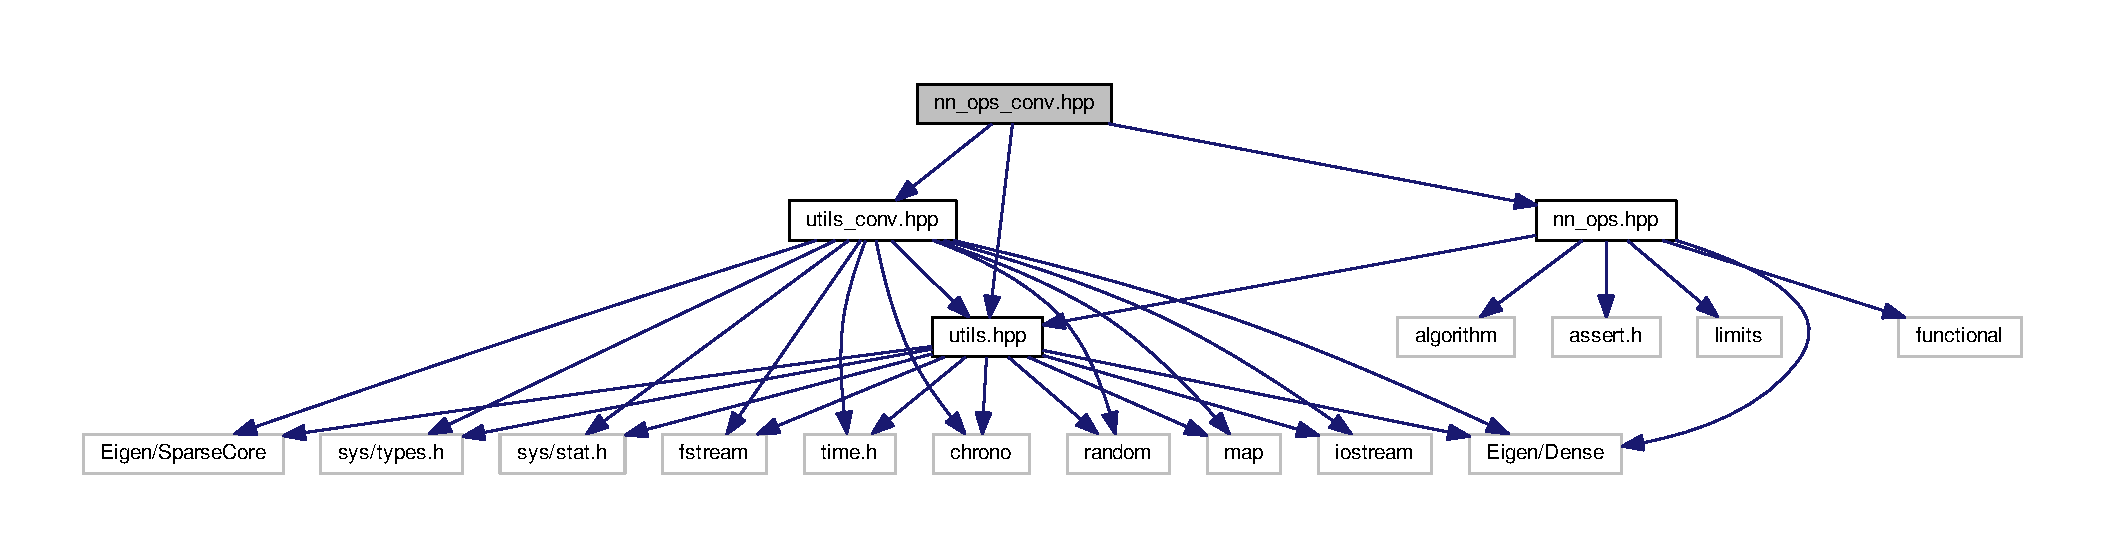
\includegraphics[width=350pt]{nn__ops__conv_8hpp__incl}
\end{center}
\end{figure}
This graph shows which files directly or indirectly include this file\+:
\nopagebreak
\begin{figure}[H]
\begin{center}
\leavevmode
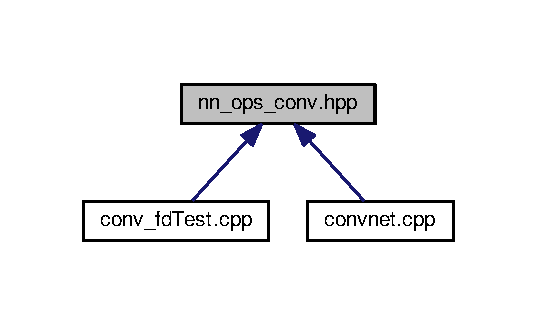
\includegraphics[width=258pt]{nn__ops__conv_8hpp__dep__incl}
\end{center}
\end{figure}
\subsection*{Functions}
\begin{DoxyCompactItemize}
\item 
void \hyperlink{nn__ops__conv_8hpp_a2d1a1a57b9ab6fcf73dac5906c9abd04}{transpose\+Conv\+W} (const My\+Matrix \&conv\+\_\+\+W, const unsigned n\+\_\+chan, const unsigned Hf, My\+Matrix \&conv\+\_\+\+W\+\_\+\+T)
\begin{DoxyCompactList}\small\item\em Transpose the convolution weights according to the characteristic of the filter. \end{DoxyCompactList}\item 
unsigned \hyperlink{nn__ops__conv_8hpp_a9e8b09d7012b01113c26ff54bd026cd9}{init\+Conv\+Layer} (const std\+::vector$<$ \hyperlink{struct_conv_layer_params}{Conv\+Layer\+Params} $>$ \&conv\+\_\+params, std\+::vector$<$ My\+Matrix $>$ \&conv\+W, std\+::vector$<$ My\+Matrix $>$ \&conv\+W\+\_\+\+T, std\+::vector$<$ My\+Vector $>$ \&conv\+B)
\begin{DoxyCompactList}\small\item\em Initialize the weights of a convolutional layer with a small normal noise (0.\+01) \end{DoxyCompactList}\item 
int \hyperlink{nn__ops__conv_8hpp_af007d6a69bc2da9b8497eaa771eb1e51}{init\+Network} (const std\+::vector$<$ unsigned $>$ \&nn\+\_\+arch, const std\+::string act\+\_\+func, const std\+::vector$<$ \hyperlink{struct_conv_layer_params}{Conv\+Layer\+Params} $>$ \&conv\+\_\+params, const std\+::vector$<$ \hyperlink{struct_pool_layer_params}{Pool\+Layer\+Params} $>$ \&pool\+\_\+params, std\+::vector$<$ My\+Matrix $>$ \&W, std\+::vector$<$ My\+Vector $>$ \&B, std\+::vector$<$ My\+Matrix $>$ \&conv\+W, std\+::vector$<$ My\+Matrix $>$ \&conv\+W\+\_\+\+T, std\+::vector$<$ My\+Vector $>$ \&conv\+B)
\begin{DoxyCompactList}\small\item\em Initialize the parameters of the convolutional Neural Network computational graph. \end{DoxyCompactList}\item 
void \hyperlink{nn__ops__conv_8hpp_a1fce4d87ddb93dde916eeafd9e724f59}{pool\+Max} (const unsigned n\+\_\+img, const unsigned conv\+\_\+\+N1, const unsigned conv\+\_\+\+N2, const unsigned F, const unsigned S, const My\+Matrix \&conv\+\_\+layer, My\+Matrix \&pool\+\_\+layer, std\+::vector$<$ unsigned $>$ \&pool\+\_\+idx\+\_\+x, std\+::vector$<$ unsigned $>$ \&pool\+\_\+idx\+\_\+y)
\begin{DoxyCompactList}\small\item\em Perform a max pooling operation. \end{DoxyCompactList}\item 
void \hyperlink{nn__ops__conv_8hpp_ab863f7d41b9e0d9d104779c802c60b4d}{conv\+Fprop} (const unsigned batch\+\_\+size, const std\+::vector$<$ \hyperlink{struct_conv_layer_params}{Conv\+Layer\+Params} $>$ \&conv\+\_\+params, const std\+::vector$<$ \hyperlink{struct_pool_layer_params}{Pool\+Layer\+Params} $>$ \&pool\+\_\+params, const Activation\+Function \&act\+\_\+func, const std\+::vector$<$ My\+Matrix $>$ \&conv\+\_\+\+W, const std\+::vector$<$ My\+Vector $>$ \&conv\+\_\+\+B, const My\+Matrix \&X\+\_\+batch, std\+::vector$<$ My\+Matrix $>$ \&conv\+\_\+\+A, std\+::vector$<$ My\+Matrix $>$ \&conv\+\_\+\+Ap, My\+Matrix \&z0, std\+::vector$<$ std\+::vector$<$ unsigned $>$$>$ \&pool\+Idx\+X, std\+::vector$<$ std\+::vector$<$ unsigned $>$$>$ \&pool\+Idx\+Y)
\begin{DoxyCompactList}\small\item\em Implementation of the forward propagation algorithm for convolutional layer. \end{DoxyCompactList}\item 
void \hyperlink{nn__ops__conv_8hpp_a86d5271f3402baee41e3e757fa2327a2}{conv\+Bprop} (const unsigned batch\+\_\+size, const std\+::vector$<$ \hyperlink{struct_conv_layer_params}{Conv\+Layer\+Params} $>$ \&conv\+\_\+params, const std\+::vector$<$ \hyperlink{struct_pool_layer_params}{Pool\+Layer\+Params} $>$ \&pool\+\_\+params, const std\+::vector$<$ My\+Matrix $>$ \&conv\+W\+\_\+\+T, const std\+::vector$<$ My\+Matrix $>$ \&conv\+Ap, const My\+Matrix \&pool\+\_\+grad\+B, std\+::vector$<$ My\+Matrix $>$ \&grad\+B, std\+::vector$<$ std\+::vector$<$ unsigned $>$$>$ \&pool\+Idx\+X, std\+::vector$<$ std\+::vector$<$ unsigned $>$$>$ \&pool\+Idx\+Y)
\begin{DoxyCompactList}\small\item\em Implementation of the backpropagation algorithm for convolutional layer. \end{DoxyCompactList}\item 
void \hyperlink{nn__ops__conv_8hpp_ac8b3063f74f3e00895c31d569c68aaa2}{conv\+Update} (const double eta, const std\+::vector$<$ My\+Matrix $>$ \&conv\+\_\+grad\+B, const std\+::vector$<$ My\+Matrix $>$ \&conv\+\_\+\+A, const My\+Matrix \&X\+\_\+batch, const std\+::string regularizer, const double lambda, std\+::vector$<$ My\+Matrix $>$ \&conv\+\_\+\+W, std\+::vector$<$ My\+Vector $>$ \&conv\+\_\+\+B)
\begin{DoxyCompactList}\small\item\em Implementation of the update function of the convolution layers (required for testing) \end{DoxyCompactList}\item 
void \hyperlink{nn__ops__conv_8hpp_a2d211cd2f6f6acab9da2c708d3cce3f2}{conv\+Update} (const unsigned batch\+\_\+size, const double eta, const std\+::vector$<$ \hyperlink{struct_conv_layer_params}{Conv\+Layer\+Params} $>$ \&conv\+\_\+params, const std\+::vector$<$ My\+Matrix $>$ \&conv\+\_\+grad\+B, const std\+::vector$<$ My\+Matrix $>$ \&conv\+\_\+\+A, const My\+Matrix \&X\+\_\+batch, const std\+::string regularizer, const double lambda, std\+::vector$<$ My\+Matrix $>$ \&conv\+\_\+\+W, std\+::vector$<$ My\+Matrix $>$ \&conv\+\_\+\+W\+\_\+\+T, std\+::vector$<$ My\+Vector $>$ \&conv\+\_\+\+B)
\begin{DoxyCompactList}\small\item\em Implementation of the update function of the convolution layers. \end{DoxyCompactList}\item 
void \hyperlink{nn__ops__conv_8hpp_a9eac26b0f319ddcafb904deca1c8a416}{conv\+Update\+Test} (const unsigned batch\+\_\+size, const double eta, const std\+::vector$<$ My\+Matrix $>$ \&conv\+\_\+grad\+B, const std\+::vector$<$ My\+Matrix $>$ \&conv\+\_\+\+A, const My\+Matrix \&X\+\_\+batch, const std\+::string regularizer, const double lambda, std\+::vector$<$ My\+Matrix $>$ \&conv\+\_\+\+W, std\+::vector$<$ My\+Vector $>$ \&conv\+\_\+\+B, std\+::vector$<$ My\+Matrix $>$ \&conv\+\_\+update, std\+::vector$<$ My\+Vector $>$ \&conv\+\_\+update\+B)
\begin{DoxyCompactList}\small\item\em Implementation of the update function of the convolution layers. \end{DoxyCompactList}\item 
\hypertarget{nn__ops__conv_8hpp_a411fe32e99240bed4d61e7dea2c3c162}{}void {\bfseries update\+Conv\+Metric} (const bool init\+\_\+flag, const double gamma, std\+::vector$<$ My\+Matrix $>$ \&conv\+\_\+\+Mii, std\+::vector$<$ My\+Matrix $>$ \&conv\+\_\+\+M0i, std\+::vector$<$ My\+Vector $>$ \&conv\+\_\+\+M00, std\+::vector$<$ My\+Matrix $>$ \&conv\+\_\+p\+Mii, std\+::vector$<$ My\+Matrix $>$ \&conv\+\_\+p\+M0i, std\+::vector$<$ My\+Vector $>$ \&conv\+\_\+p\+M00)\label{nn__ops__conv_8hpp_a411fe32e99240bed4d61e7dea2c3c162}

\item 
\hypertarget{nn__ops__conv_8hpp_aa252e74b217c2b2665954a2a39f798f9}{}void {\bfseries build\+Conv\+Q\+D\+Metric} (const unsigned batch\+\_\+size, const std\+::vector$<$ My\+Matrix $>$ \&conv\+\_\+grad\+B\+\_\+sq, const std\+::vector$<$ My\+Matrix $>$ \&conv\+\_\+\+A, const My\+Matrix \&X\+\_\+batch, const std\+::vector$<$ My\+Matrix $>$ \&conv\+\_\+\+W, const double mat\+\_\+reg, std\+::vector$<$ My\+Matrix $>$ \&conv\+\_\+\+Mii, std\+::vector$<$ My\+Matrix $>$ \&conv\+\_\+\+M0i, std\+::vector$<$ My\+Vector $>$ \&conv\+\_\+\+M00)\label{nn__ops__conv_8hpp_aa252e74b217c2b2665954a2a39f798f9}

\item 
\hypertarget{nn__ops__conv_8hpp_abbc7097bec6fae0caa783efc405cf277}{}void {\bfseries compute\+Loss} (const Activation\+Function \&act\+\_\+func, const unsigned batch\+\_\+size, const My\+Matrix \&X, const My\+Vector \&Y, const std\+::vector$<$ \hyperlink{struct_conv_layer_params}{Conv\+Layer\+Params} $>$ \&conv\+\_\+params, const std\+::vector$<$ \hyperlink{struct_pool_layer_params}{Pool\+Layer\+Params} $>$ \&pool\+\_\+params, const std\+::vector$<$ My\+Matrix $>$ \&conv\+\_\+\+W, const std\+::vector$<$ My\+Vector $>$ \&conv\+\_\+\+B, const std\+::vector$<$ My\+Matrix $>$ \&W, const std\+::vector$<$ My\+Vector $>$ \&B, double \&loss, double \&accuracy)\label{nn__ops__conv_8hpp_abbc7097bec6fae0caa783efc405cf277}

\item 
\hypertarget{nn__ops__conv_8hpp_a6657175f9e911da675e3c637d0e275d2}{}void {\bfseries eval\+Model} (const Activation\+Function \&eval\+\_\+act\+\_\+func, const \hyperlink{struct_params}{Params} \&params, const unsigned n\+\_\+batch, const unsigned batch\+\_\+size, const unsigned n\+\_\+example, const My\+Matrix \&X, const My\+Vector \&Y, const std\+::vector$<$ \hyperlink{struct_conv_layer_params}{Conv\+Layer\+Params} $>$ \&conv\+\_\+params, const std\+::vector$<$ \hyperlink{struct_pool_layer_params}{Pool\+Layer\+Params} $>$ \&pool\+\_\+params, const std\+::vector$<$ My\+Matrix $>$ \&conv\+\_\+\+W, const std\+::vector$<$ My\+Vector $>$ \&conv\+\_\+\+B, std\+::vector$<$ My\+Matrix $>$ \&W\+\_\+eval, std\+::vector$<$ My\+Vector $>$ \&B, double \&acc\+\_\+loss, double \&acc\+\_\+accuracy)\label{nn__ops__conv_8hpp_a6657175f9e911da675e3c637d0e275d2}

\item 
\hypertarget{nn__ops__conv_8hpp_ad0afdaae88b522aa8b71559b71c758cd}{}void {\bfseries eval\+Model} (const Activation\+Function \&eval\+\_\+act\+\_\+func, const unsigned train\+\_\+batch\+\_\+size, const My\+Matrix \&X\+\_\+train, const My\+Matrix \&Y\+\_\+train, const unsigned valid\+\_\+batch\+\_\+size, const My\+Matrix \&X\+\_\+valid, const My\+Matrix \&Y\+\_\+valid, const std\+::vector$<$ \hyperlink{struct_conv_layer_params}{Conv\+Layer\+Params} $>$ \&conv\+\_\+params, const std\+::vector$<$ \hyperlink{struct_pool_layer_params}{Pool\+Layer\+Params} $>$ \&pool\+\_\+params, const std\+::vector$<$ My\+Matrix $>$ \&conv\+\_\+\+W, const std\+::vector$<$ My\+Vector $>$ \&conv\+\_\+\+B, std\+::vector$<$ My\+Matrix $>$ \&W\+\_\+eval, std\+::vector$<$ My\+Vector $>$ \&B, double \&train\+\_\+loss, double \&train\+\_\+accuracy, double \&valid\+\_\+loss, double \&valid\+\_\+accuracy)\label{nn__ops__conv_8hpp_ad0afdaae88b522aa8b71559b71c758cd}

\end{DoxyCompactItemize}


\subsection{Detailed Description}
Implementation of the functions required for convolutional neural networks. 

\begin{DoxyAuthor}{Author}
Gaetan Marceau Caron \& Yann Ollivier 
\end{DoxyAuthor}
\begin{DoxyVersion}{Version}
1.\+0 
\end{DoxyVersion}


\subsection{Function Documentation}
\hypertarget{nn__ops__conv_8hpp_a86d5271f3402baee41e3e757fa2327a2}{}\index{nn\+\_\+ops\+\_\+conv.\+hpp@{nn\+\_\+ops\+\_\+conv.\+hpp}!conv\+Bprop@{conv\+Bprop}}
\index{conv\+Bprop@{conv\+Bprop}!nn\+\_\+ops\+\_\+conv.\+hpp@{nn\+\_\+ops\+\_\+conv.\+hpp}}
\subsubsection[{conv\+Bprop}]{\setlength{\rightskip}{0pt plus 5cm}void conv\+Bprop (
\begin{DoxyParamCaption}
\item[{const unsigned}]{batch\+\_\+size, }
\item[{const std\+::vector$<$ {\bf Conv\+Layer\+Params} $>$ \&}]{conv\+\_\+params, }
\item[{const std\+::vector$<$ {\bf Pool\+Layer\+Params} $>$ \&}]{pool\+\_\+params, }
\item[{const std\+::vector$<$ My\+Matrix $>$ \&}]{conv\+W\+\_\+\+T, }
\item[{const std\+::vector$<$ My\+Matrix $>$ \&}]{conv\+Ap, }
\item[{const My\+Matrix \&}]{pool\+\_\+grad\+B, }
\item[{std\+::vector$<$ My\+Matrix $>$ \&}]{grad\+B, }
\item[{std\+::vector$<$ std\+::vector$<$ unsigned $>$$>$ \&}]{pool\+Idx\+X, }
\item[{std\+::vector$<$ std\+::vector$<$ unsigned $>$$>$ \&}]{pool\+Idx\+Y}
\end{DoxyParamCaption}
)}\label{nn__ops__conv_8hpp_a86d5271f3402baee41e3e757fa2327a2}


Implementation of the backpropagation algorithm for convolutional layer. 


\begin{DoxyParams}{Parameters}
{\em batch\+\_\+size} & number of examples in the batch \\
\hline
{\em conv\+\_\+params} & a standard vector with parameters for each convolutional layer \\
\hline
{\em pool\+\_\+params} & a standard vector with parameters for each pooling layer \\
\hline
{\em conv\+W\+\_\+\+T} & a standard vector of bias vectors (one per layer) \\
\hline
{\em conv\+Ap} & \\
\hline
{\em pool\+\_\+grad\+B} & \\
\hline
{\em grad\+B} & \\
\hline
{\em pool\+Idx\+X} & \\
\hline
{\em pool\+Idx\+Y} & \\
\hline
\end{DoxyParams}
\hypertarget{nn__ops__conv_8hpp_ab863f7d41b9e0d9d104779c802c60b4d}{}\index{nn\+\_\+ops\+\_\+conv.\+hpp@{nn\+\_\+ops\+\_\+conv.\+hpp}!conv\+Fprop@{conv\+Fprop}}
\index{conv\+Fprop@{conv\+Fprop}!nn\+\_\+ops\+\_\+conv.\+hpp@{nn\+\_\+ops\+\_\+conv.\+hpp}}
\subsubsection[{conv\+Fprop}]{\setlength{\rightskip}{0pt plus 5cm}void conv\+Fprop (
\begin{DoxyParamCaption}
\item[{const unsigned}]{batch\+\_\+size, }
\item[{const std\+::vector$<$ {\bf Conv\+Layer\+Params} $>$ \&}]{conv\+\_\+params, }
\item[{const std\+::vector$<$ {\bf Pool\+Layer\+Params} $>$ \&}]{pool\+\_\+params, }
\item[{const Activation\+Function \&}]{act\+\_\+func, }
\item[{const std\+::vector$<$ My\+Matrix $>$ \&}]{conv\+\_\+\+W, }
\item[{const std\+::vector$<$ My\+Vector $>$ \&}]{conv\+\_\+\+B, }
\item[{const My\+Matrix \&}]{X\+\_\+batch, }
\item[{std\+::vector$<$ My\+Matrix $>$ \&}]{conv\+\_\+\+A, }
\item[{std\+::vector$<$ My\+Matrix $>$ \&}]{conv\+\_\+\+Ap, }
\item[{My\+Matrix \&}]{z0, }
\item[{std\+::vector$<$ std\+::vector$<$ unsigned $>$$>$ \&}]{pool\+Idx\+X, }
\item[{std\+::vector$<$ std\+::vector$<$ unsigned $>$$>$ \&}]{pool\+Idx\+Y}
\end{DoxyParamCaption}
)}\label{nn__ops__conv_8hpp_ab863f7d41b9e0d9d104779c802c60b4d}


Implementation of the forward propagation algorithm for convolutional layer. 


\begin{DoxyParams}{Parameters}
{\em batch\+\_\+size} & number of examples in the batch \\
\hline
{\em conv\+\_\+params} & a standard vector with parameters for each convolutional layer \\
\hline
{\em pool\+\_\+params} & a standard vector with parameters for each pooling layer \\
\hline
{\em act\+\_\+func} & string representing the activation function \\
\hline
{\em conv\+\_\+\+W} & \\
\hline
{\em conv\+\_\+\+B} & \\
\hline
{\em X\+\_\+batch} & a matrix containing the training examples of the current minibatch \\
\hline
{\em conv\+\_\+\+A} & \\
\hline
{\em conv\+\_\+d\+A} & \\
\hline
{\em z0} & \\
\hline
{\em pool\+Idx\+X} & \\
\hline
{\em pool\+Idx\+Y} & \\
\hline
\end{DoxyParams}
\hypertarget{nn__ops__conv_8hpp_ac8b3063f74f3e00895c31d569c68aaa2}{}\index{nn\+\_\+ops\+\_\+conv.\+hpp@{nn\+\_\+ops\+\_\+conv.\+hpp}!conv\+Update@{conv\+Update}}
\index{conv\+Update@{conv\+Update}!nn\+\_\+ops\+\_\+conv.\+hpp@{nn\+\_\+ops\+\_\+conv.\+hpp}}
\subsubsection[{conv\+Update}]{\setlength{\rightskip}{0pt plus 5cm}void conv\+Update (
\begin{DoxyParamCaption}
\item[{const double}]{eta, }
\item[{const std\+::vector$<$ My\+Matrix $>$ \&}]{conv\+\_\+grad\+B, }
\item[{const std\+::vector$<$ My\+Matrix $>$ \&}]{conv\+\_\+\+A, }
\item[{const My\+Matrix \&}]{X\+\_\+batch, }
\item[{const std\+::string}]{regularizer, }
\item[{const double}]{lambda, }
\item[{std\+::vector$<$ My\+Matrix $>$ \&}]{conv\+\_\+\+W, }
\item[{std\+::vector$<$ My\+Vector $>$ \&}]{conv\+\_\+\+B}
\end{DoxyParamCaption}
)}\label{nn__ops__conv_8hpp_ac8b3063f74f3e00895c31d569c68aaa2}


Implementation of the update function of the convolution layers (required for testing) 


\begin{DoxyParams}{Parameters}
{\em eta} & the gradient descent step-\/size \\
\hline
{\em conv\+\_\+grad\+B} & a standard vector of the gradient w.\+r.\+t. the pre-\/activation values (one per conv layer) \\
\hline
{\em conv\+\_\+\+A} & a standard vector of activation values (one per conv layer) \\
\hline
{\em X\+\_\+batch} & a matrix containing the training examples of the current minibatch \\
\hline
{\em regularizer} & the string of the norm regularizer (L1 or L2) \\
\hline
{\em lambda} & the amplitude of the regularization term \\
\hline
{\em conv\+\_\+\+W} & a standard vector of weight matrices (one per conv layer) \\
\hline
{\em conv\+\_\+\+B} & a standard vector of bias vectors (one per conv layer) \\
\hline
\end{DoxyParams}
\hypertarget{nn__ops__conv_8hpp_a2d211cd2f6f6acab9da2c708d3cce3f2}{}\index{nn\+\_\+ops\+\_\+conv.\+hpp@{nn\+\_\+ops\+\_\+conv.\+hpp}!conv\+Update@{conv\+Update}}
\index{conv\+Update@{conv\+Update}!nn\+\_\+ops\+\_\+conv.\+hpp@{nn\+\_\+ops\+\_\+conv.\+hpp}}
\subsubsection[{conv\+Update}]{\setlength{\rightskip}{0pt plus 5cm}void conv\+Update (
\begin{DoxyParamCaption}
\item[{const unsigned}]{batch\+\_\+size, }
\item[{const double}]{eta, }
\item[{const std\+::vector$<$ {\bf Conv\+Layer\+Params} $>$ \&}]{conv\+\_\+params, }
\item[{const std\+::vector$<$ My\+Matrix $>$ \&}]{conv\+\_\+grad\+B, }
\item[{const std\+::vector$<$ My\+Matrix $>$ \&}]{conv\+\_\+\+A, }
\item[{const My\+Matrix \&}]{X\+\_\+batch, }
\item[{const std\+::string}]{regularizer, }
\item[{const double}]{lambda, }
\item[{std\+::vector$<$ My\+Matrix $>$ \&}]{conv\+\_\+\+W, }
\item[{std\+::vector$<$ My\+Matrix $>$ \&}]{conv\+\_\+\+W\+\_\+\+T, }
\item[{std\+::vector$<$ My\+Vector $>$ \&}]{conv\+\_\+\+B}
\end{DoxyParamCaption}
)}\label{nn__ops__conv_8hpp_a2d211cd2f6f6acab9da2c708d3cce3f2}


Implementation of the update function of the convolution layers. 


\begin{DoxyParams}{Parameters}
{\em batch\+\_\+size} & number of examples in the batch \\
\hline
{\em eta} & the gradient descent step-\/size \\
\hline
{\em conv\+\_\+grad\+B} & a standard vector of the gradient w.\+r.\+t. the pre-\/activation values (one per conv layer) \\
\hline
{\em conv\+\_\+\+A} & a standard vector of activation values (one per conv layer) \\
\hline
{\em X\+\_\+batch} & a matrix containing the training examples of the current minibatch \\
\hline
{\em regularizer} & the string of the norm regularizer (L1 or L2) \\
\hline
{\em lambda} & the amplitude of the regularization term \\
\hline
{\em conv\+\_\+\+W} & a standard vector of weight matrices (one per conv layer) \\
\hline
{\em conv\+\_\+\+B} & a standard vector of bias vectors (one per conv layer) \\
\hline
\end{DoxyParams}
\hypertarget{nn__ops__conv_8hpp_a9eac26b0f319ddcafb904deca1c8a416}{}\index{nn\+\_\+ops\+\_\+conv.\+hpp@{nn\+\_\+ops\+\_\+conv.\+hpp}!conv\+Update\+Test@{conv\+Update\+Test}}
\index{conv\+Update\+Test@{conv\+Update\+Test}!nn\+\_\+ops\+\_\+conv.\+hpp@{nn\+\_\+ops\+\_\+conv.\+hpp}}
\subsubsection[{conv\+Update\+Test}]{\setlength{\rightskip}{0pt plus 5cm}void conv\+Update\+Test (
\begin{DoxyParamCaption}
\item[{const unsigned}]{batch\+\_\+size, }
\item[{const double}]{eta, }
\item[{const std\+::vector$<$ My\+Matrix $>$ \&}]{conv\+\_\+grad\+B, }
\item[{const std\+::vector$<$ My\+Matrix $>$ \&}]{conv\+\_\+\+A, }
\item[{const My\+Matrix \&}]{X\+\_\+batch, }
\item[{const std\+::string}]{regularizer, }
\item[{const double}]{lambda, }
\item[{std\+::vector$<$ My\+Matrix $>$ \&}]{conv\+\_\+\+W, }
\item[{std\+::vector$<$ My\+Vector $>$ \&}]{conv\+\_\+\+B, }
\item[{std\+::vector$<$ My\+Matrix $>$ \&}]{conv\+\_\+update, }
\item[{std\+::vector$<$ My\+Vector $>$ \&}]{conv\+\_\+update\+B}
\end{DoxyParamCaption}
)}\label{nn__ops__conv_8hpp_a9eac26b0f319ddcafb904deca1c8a416}


Implementation of the update function of the convolution layers. 


\begin{DoxyParams}{Parameters}
{\em batch\+\_\+size} & number of examples in the batch \\
\hline
{\em eta} & the gradient descent step-\/size \\
\hline
{\em conv\+\_\+grad\+B} & a standard vector of the gradient w.\+r.\+t. the pre-\/activation values (one per conv layer) \\
\hline
{\em conv\+\_\+\+A} & a standard vector of activation values (one per conv layer) \\
\hline
{\em X\+\_\+batch} & a matrix containing the training examples of the current minibatch \\
\hline
{\em regularizer} & the string of the norm regularizer (L1 or L2) \\
\hline
{\em lambda} & the amplitude of the regularization term \\
\hline
{\em conv\+\_\+\+W} & a standard vector of weight matrices (one per conv layer) \\
\hline
{\em conv\+\_\+\+B} & a standard vector of bias vectors (one per conv layer) \\
\hline
\end{DoxyParams}
\hypertarget{nn__ops__conv_8hpp_a9e8b09d7012b01113c26ff54bd026cd9}{}\index{nn\+\_\+ops\+\_\+conv.\+hpp@{nn\+\_\+ops\+\_\+conv.\+hpp}!init\+Conv\+Layer@{init\+Conv\+Layer}}
\index{init\+Conv\+Layer@{init\+Conv\+Layer}!nn\+\_\+ops\+\_\+conv.\+hpp@{nn\+\_\+ops\+\_\+conv.\+hpp}}
\subsubsection[{init\+Conv\+Layer}]{\setlength{\rightskip}{0pt plus 5cm}unsigned init\+Conv\+Layer (
\begin{DoxyParamCaption}
\item[{const std\+::vector$<$ {\bf Conv\+Layer\+Params} $>$ \&}]{conv\+\_\+params, }
\item[{std\+::vector$<$ My\+Matrix $>$ \&}]{conv\+W, }
\item[{std\+::vector$<$ My\+Matrix $>$ \&}]{conv\+W\+\_\+\+T, }
\item[{std\+::vector$<$ My\+Vector $>$ \&}]{conv\+B}
\end{DoxyParamCaption}
)}\label{nn__ops__conv_8hpp_a9e8b09d7012b01113c26ff54bd026cd9}


Initialize the weights of a convolutional layer with a small normal noise (0.\+01) 


\begin{DoxyParams}{Parameters}
{\em conv\+\_\+params} & a standard vector with parameters for each convolutional layer \\
\hline
{\em conv\+W} & a standard vector with weight matrix for each convolutional layer \\
\hline
{\em conv\+W\+\_\+\+T} & a standard vector with transposed weight matrix for each convolutional layer \\
\hline
{\em conv\+B} & a standard vector with bias vector for each convolutional layer \\
\hline
\end{DoxyParams}
\hypertarget{nn__ops__conv_8hpp_af007d6a69bc2da9b8497eaa771eb1e51}{}\index{nn\+\_\+ops\+\_\+conv.\+hpp@{nn\+\_\+ops\+\_\+conv.\+hpp}!init\+Network@{init\+Network}}
\index{init\+Network@{init\+Network}!nn\+\_\+ops\+\_\+conv.\+hpp@{nn\+\_\+ops\+\_\+conv.\+hpp}}
\subsubsection[{init\+Network}]{\setlength{\rightskip}{0pt plus 5cm}int init\+Network (
\begin{DoxyParamCaption}
\item[{const std\+::vector$<$ unsigned $>$ \&}]{nn\+\_\+arch, }
\item[{const std\+::string}]{act\+\_\+func, }
\item[{const std\+::vector$<$ {\bf Conv\+Layer\+Params} $>$ \&}]{conv\+\_\+params, }
\item[{const std\+::vector$<$ {\bf Pool\+Layer\+Params} $>$ \&}]{pool\+\_\+params, }
\item[{std\+::vector$<$ My\+Matrix $>$ \&}]{W, }
\item[{std\+::vector$<$ My\+Vector $>$ \&}]{B, }
\item[{std\+::vector$<$ My\+Matrix $>$ \&}]{conv\+W, }
\item[{std\+::vector$<$ My\+Matrix $>$ \&}]{conv\+W\+\_\+\+T, }
\item[{std\+::vector$<$ My\+Vector $>$ \&}]{conv\+B}
\end{DoxyParamCaption}
)}\label{nn__ops__conv_8hpp_af007d6a69bc2da9b8497eaa771eb1e51}


Initialize the parameters of the convolutional Neural Network computational graph. 


\begin{DoxyParams}{Parameters}
{\em nn\+\_\+arch} & number of activation units for each layer \\
\hline
{\em act\+\_\+func} & string representing the activation function \\
\hline
{\em conv\+\_\+params} & a standard vector with parameters for each convolutional layer \\
\hline
{\em pool\+\_\+params} & a standard vector with parameters for each pooling layer \\
\hline
{\em W} & a standard vector of weight matrices (one per layer) \\
\hline
{\em B} & a standard vector of bias vectors (one per layer) \\
\hline
{\em conv\+W} & a standard vector of weight matrices (one per layer) \\
\hline
{\em conv\+W\+\_\+\+T} & a standard vector of bias vectors (one per layer) \\
\hline
{\em conv\+B} & a standard vector of weight matrices (one per layer) \\
\hline
\end{DoxyParams}
\begin{DoxyReturn}{Returns}
the number of parameters 
\end{DoxyReturn}
\hypertarget{nn__ops__conv_8hpp_a1fce4d87ddb93dde916eeafd9e724f59}{}\index{nn\+\_\+ops\+\_\+conv.\+hpp@{nn\+\_\+ops\+\_\+conv.\+hpp}!pool\+Max@{pool\+Max}}
\index{pool\+Max@{pool\+Max}!nn\+\_\+ops\+\_\+conv.\+hpp@{nn\+\_\+ops\+\_\+conv.\+hpp}}
\subsubsection[{pool\+Max}]{\setlength{\rightskip}{0pt plus 5cm}void pool\+Max (
\begin{DoxyParamCaption}
\item[{const unsigned}]{n\+\_\+img, }
\item[{const unsigned}]{conv\+\_\+\+N1, }
\item[{const unsigned}]{conv\+\_\+\+N2, }
\item[{const unsigned}]{F, }
\item[{const unsigned}]{S, }
\item[{const My\+Matrix \&}]{conv\+\_\+layer, }
\item[{My\+Matrix \&}]{pool\+\_\+layer, }
\item[{std\+::vector$<$ unsigned $>$ \&}]{pool\+\_\+idx\+\_\+x, }
\item[{std\+::vector$<$ unsigned $>$ \&}]{pool\+\_\+idx\+\_\+y}
\end{DoxyParamCaption}
)}\label{nn__ops__conv_8hpp_a1fce4d87ddb93dde916eeafd9e724f59}


Perform a max pooling operation. 


\begin{DoxyParams}{Parameters}
{\em n\+\_\+img} & the number of images \\
\hline
{\em conv\+\_\+\+N1} & \\
\hline
{\em conv\+\_\+\+N2} & \\
\hline
{\em F} & \\
\hline
{\em S} & \\
\hline
{\em conv\+\_\+layer} & \\
\hline
{\em pool\+\_\+layer} & \\
\hline
{\em pool\+\_\+idx\+\_\+x} & \\
\hline
{\em pool\+\_\+idx\+\_\+y} & \\
\hline
\end{DoxyParams}
\hypertarget{nn__ops__conv_8hpp_a2d1a1a57b9ab6fcf73dac5906c9abd04}{}\index{nn\+\_\+ops\+\_\+conv.\+hpp@{nn\+\_\+ops\+\_\+conv.\+hpp}!transpose\+Conv\+W@{transpose\+Conv\+W}}
\index{transpose\+Conv\+W@{transpose\+Conv\+W}!nn\+\_\+ops\+\_\+conv.\+hpp@{nn\+\_\+ops\+\_\+conv.\+hpp}}
\subsubsection[{transpose\+Conv\+W}]{\setlength{\rightskip}{0pt plus 5cm}void transpose\+Conv\+W (
\begin{DoxyParamCaption}
\item[{const My\+Matrix \&}]{conv\+\_\+\+W, }
\item[{const unsigned}]{n\+\_\+chan, }
\item[{const unsigned}]{Hf, }
\item[{My\+Matrix \&}]{conv\+\_\+\+W\+\_\+\+T}
\end{DoxyParamCaption}
)}\label{nn__ops__conv_8hpp_a2d1a1a57b9ab6fcf73dac5906c9abd04}


Transpose the convolution weights according to the characteristic of the filter. 


\begin{DoxyParams}{Parameters}
{\em conv\+\_\+\+W} & a weight matrix of a convolutional layer \\
\hline
{\em n\+\_\+chan} & the number of channels \\
\hline
{\em Hf} & the size of the filter \\
\hline
{\em conv\+\_\+\+W\+\_\+\+T} & the transposed weight matrix of a convolutional layer \\
\hline
\end{DoxyParams}

\hypertarget{nn__ops__sp__conv_8hpp}{}\section{nn\+\_\+ops\+\_\+sp\+\_\+conv.\+hpp File Reference}
\label{nn__ops__sp__conv_8hpp}\index{nn\+\_\+ops\+\_\+sp\+\_\+conv.\+hpp@{nn\+\_\+ops\+\_\+sp\+\_\+conv.\+hpp}}


Implementation of the functions required for neural networks.  


{\ttfamily \#include $<$functional$>$}\\*
{\ttfamily \#include $<$Eigen/\+Dense$>$}\\*
{\ttfamily \#include $<$Eigen/\+Sparse\+Core$>$}\\*
{\ttfamily \#include $<$algorithm$>$}\\*
{\ttfamily \#include $<$assert.\+h$>$}\\*
{\ttfamily \#include $<$limits$>$}\\*
{\ttfamily \#include \char`\"{}utils.\+hpp\char`\"{}}\\*
Include dependency graph for nn\+\_\+ops\+\_\+sp\+\_\+conv.\+hpp\+:
\nopagebreak
\begin{figure}[H]
\begin{center}
\leavevmode
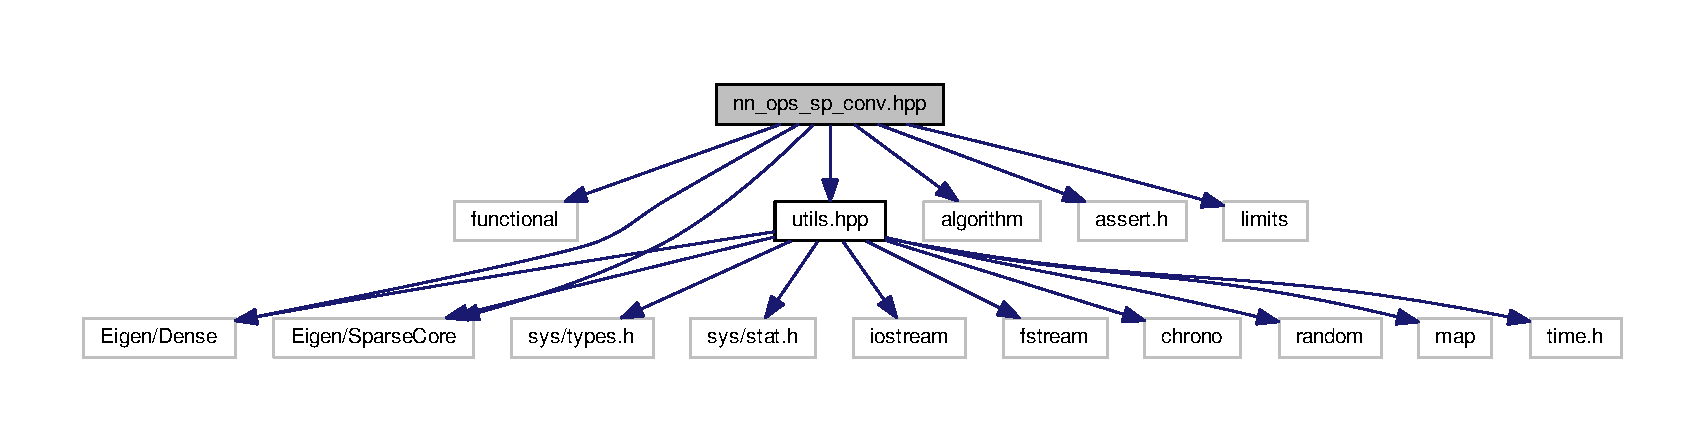
\includegraphics[width=350pt]{nn__ops__sp__conv_8hpp__incl}
\end{center}
\end{figure}
\subsection*{Functions}
\begin{DoxyCompactItemize}
\item 
\hypertarget{nn__ops__sp__conv_8hpp_a098dfb7eceed6e3e86c4866ffd2369d1}{}void {\bfseries init\+Sliding\+Metric} (const std\+::vector$<$ My\+Matrix $>$ \&W, std\+::vector$<$ My\+Matrix $>$ \&p\+Mii, std\+::vector$<$ My\+Matrix $>$ \&p\+M0i, std\+::vector$<$ My\+Vector $>$ \&p\+M00)\label{nn__ops__sp__conv_8hpp_a098dfb7eceed6e3e86c4866ffd2369d1}

\item 
\hypertarget{nn__ops__sp__conv_8hpp_a2d1a1a57b9ab6fcf73dac5906c9abd04}{}void {\bfseries transpose\+Conv\+W} (const My\+Matrix \&conv\+\_\+\+W, const unsigned n\+\_\+chan, const unsigned Hf, My\+Matrix \&conv\+\_\+\+W\+\_\+\+T)\label{nn__ops__sp__conv_8hpp_a2d1a1a57b9ab6fcf73dac5906c9abd04}

\item 
\hypertarget{nn__ops__sp__conv_8hpp_a91189f463ca2a137929752d66328acc5}{}void {\bfseries init\+Full\+Layer} (const unsigned n\+\_\+act0, const unsigned n\+\_\+act1, const double sigma, My\+Matrix \&W)\label{nn__ops__sp__conv_8hpp_a91189f463ca2a137929752d66328acc5}

\item 
\hypertarget{nn__ops__sp__conv_8hpp_ac180a953c780bb98064e69c211d59dc9}{}void {\bfseries init\+Sparse\+Layer} (const unsigned sparsity, const unsigned n\+\_\+act0, const unsigned n\+\_\+act1, const double sigma, unsigned \&param\+\_\+counter, std\+::vector$<$ Sp\+Entry $>$ \&coeff)\label{nn__ops__sp__conv_8hpp_ac180a953c780bb98064e69c211d59dc9}

\item 
\hypertarget{nn__ops__sp__conv_8hpp_a9e8b09d7012b01113c26ff54bd026cd9}{}unsigned {\bfseries init\+Conv\+Layer} (const std\+::vector$<$ \hyperlink{struct_conv_layer_params}{Conv\+Layer\+Params} $>$ \&conv\+\_\+params, std\+::vector$<$ My\+Matrix $>$ \&conv\+W, std\+::vector$<$ My\+Matrix $>$ \&conv\+W\+\_\+\+T, std\+::vector$<$ My\+Vector $>$ \&conv\+B)\label{nn__ops__sp__conv_8hpp_a9e8b09d7012b01113c26ff54bd026cd9}

\item 
\hypertarget{nn__ops__sp__conv_8hpp_afd66654e77a1b2693290002af0efbac1}{}int {\bfseries init\+Network} (const std\+::vector$<$ unsigned $>$ \&nn\+\_\+arch, const std\+::string act\+\_\+func, const unsigned sparsity, const std\+::vector$<$ \hyperlink{struct_conv_layer_params}{Conv\+Layer\+Params} $>$ \&conv\+\_\+params, const std\+::vector$<$ \hyperlink{struct_pool_layer_params}{Pool\+Layer\+Params} $>$ \&pool\+\_\+params, My\+Matrix \&W\+\_\+out, std\+::vector$<$ My\+Sp\+Matrix $>$ \&W, std\+::vector$<$ My\+Sp\+Matrix $>$ \&Wt, std\+::vector$<$ My\+Vector $>$ \&B, std\+::vector$<$ My\+Matrix $>$ \&conv\+W, std\+::vector$<$ My\+Matrix $>$ \&conv\+W\+\_\+\+T, std\+::vector$<$ My\+Vector $>$ \&conv\+B)\label{nn__ops__sp__conv_8hpp_afd66654e77a1b2693290002af0efbac1}

\item 
\hypertarget{nn__ops__sp__conv_8hpp_a22f109ce3d23796de9d34fb9eee73040}{}double {\bfseries sign\+Func} (double x)\label{nn__ops__sp__conv_8hpp_a22f109ce3d23796de9d34fb9eee73040}

\item 
\hypertarget{nn__ops__sp__conv_8hpp_a03a2f1c37574a2bc61630b6e5bf86dcf}{}double {\bfseries square\+Func} (double x)\label{nn__ops__sp__conv_8hpp_a03a2f1c37574a2bc61630b6e5bf86dcf}

\item 
\hypertarget{nn__ops__sp__conv_8hpp_a6ceeb10733d64ab2587e136e884c2ec8}{}double {\bfseries sqrt\+Func} (double x)\label{nn__ops__sp__conv_8hpp_a6ceeb10733d64ab2587e136e884c2ec8}

\item 
\hypertarget{nn__ops__sp__conv_8hpp_a6bac3899a024aa93b77e99e169f1e86c}{}double {\bfseries sum\+Cst\+Func} (double x, double cst)\label{nn__ops__sp__conv_8hpp_a6bac3899a024aa93b77e99e169f1e86c}

\item 
\hypertarget{nn__ops__sp__conv_8hpp_a4c86f2557fe76d7b0ca7c5111eb7927b}{}void {\bfseries softmax} (const My\+Matrix \&a, My\+Matrix \&out)\label{nn__ops__sp__conv_8hpp_a4c86f2557fe76d7b0ca7c5111eb7927b}

\item 
\hypertarget{nn__ops__sp__conv_8hpp_aa125fb3ba2bec422df3857be6097239a}{}void \hyperlink{nn__ops__sp__conv_8hpp_aa125fb3ba2bec422df3857be6097239a}{logistic} (const bool deriv\+\_\+flag, const My\+Matrix \&z, My\+Matrix \&a, My\+Matrix \&ap)\label{nn__ops__sp__conv_8hpp_aa125fb3ba2bec422df3857be6097239a}

\begin{DoxyCompactList}\small\item\em Activation functions. \end{DoxyCompactList}\item 
\hypertarget{nn__ops__sp__conv_8hpp_aea7d4da56658e748deb416a1a132700a}{}void {\bfseries my\+\_\+tanh} (const bool deriv\+\_\+flag, const My\+Matrix \&z, My\+Matrix \&a, My\+Matrix \&ap)\label{nn__ops__sp__conv_8hpp_aea7d4da56658e748deb416a1a132700a}

\item 
\hypertarget{nn__ops__sp__conv_8hpp_a7ee597a1779e64682c57c86576964432}{}void {\bfseries relu} (const bool deriv\+\_\+flag, const My\+Matrix \&z, My\+Matrix \&a, My\+Matrix \&ap)\label{nn__ops__sp__conv_8hpp_a7ee597a1779e64682c57c86576964432}

\item 
\hypertarget{nn__ops__sp__conv_8hpp_ac56dfda8be864dadf5db85c56978171d}{}void {\bfseries dropout} (const double prob, My\+Matrix \&A, My\+Matrix \&B)\label{nn__ops__sp__conv_8hpp_ac56dfda8be864dadf5db85c56978171d}

\item 
\hypertarget{nn__ops__sp__conv_8hpp_afe6393d9948ae9a81cb1292aad353c48}{}void {\bfseries dropout} (const double prob, My\+Matrix \&A)\label{nn__ops__sp__conv_8hpp_afe6393d9948ae9a81cb1292aad353c48}

\item 
\hypertarget{nn__ops__sp__conv_8hpp_ab3c3dfed86a314f2df7557c50cd455d7}{}void {\bfseries build\+Conv\+Matrix} (const unsigned n\+\_\+img, const unsigned conv\+\_\+\+N1, const unsigned conv\+\_\+\+N2, const unsigned F, const unsigned S, const unsigned P, const My\+Matrix \&conv\+\_\+layer, My\+Matrix \&conv\+\_\+matrix)\label{nn__ops__sp__conv_8hpp_ab3c3dfed86a314f2df7557c50cd455d7}

\item 
\hypertarget{nn__ops__sp__conv_8hpp_a1fce4d87ddb93dde916eeafd9e724f59}{}void {\bfseries pool\+Max} (const unsigned n\+\_\+img, const unsigned conv\+\_\+\+N1, const unsigned conv\+\_\+\+N2, const unsigned F, const unsigned S, const My\+Matrix \&conv\+\_\+layer, My\+Matrix \&pool\+\_\+layer, std\+::vector$<$ unsigned $>$ \&pool\+\_\+idx\+\_\+x, std\+::vector$<$ unsigned $>$ \&pool\+\_\+idx\+\_\+y)\label{nn__ops__sp__conv_8hpp_a1fce4d87ddb93dde916eeafd9e724f59}

\item 
\hypertarget{nn__ops__sp__conv_8hpp_ad89e254b0d693484e43a8fc7d73b11db}{}void {\bfseries fprop} (const bool dropout\+\_\+flag, const Activation\+Function \&act\+\_\+func, const std\+::vector$<$ My\+Sp\+Matrix $>$ \&W, const My\+Matrix \&W\+\_\+out, const std\+::vector$<$ My\+Vector $>$ \&B, const My\+Matrix \&X\+\_\+batch, std\+::vector$<$ My\+Matrix $>$ \&Z, std\+::vector$<$ My\+Matrix $>$ \&A, std\+::vector$<$ My\+Matrix $>$ \&Ap)\label{nn__ops__sp__conv_8hpp_ad89e254b0d693484e43a8fc7d73b11db}

\item 
\hypertarget{nn__ops__sp__conv_8hpp_a14a70839d56b16d2e5fe814a2d1079e8}{}void {\bfseries fprop} (const bool dropout\+\_\+flag, const Activation\+Function \&act\+\_\+func, const std\+::vector$<$ My\+Matrix $>$ \&W, const std\+::vector$<$ My\+Vector $>$ \&B, const My\+Matrix \&X\+\_\+batch, std\+::vector$<$ My\+Matrix $>$ \&Z, std\+::vector$<$ My\+Matrix $>$ \&A, std\+::vector$<$ My\+Matrix $>$ \&Ap)\label{nn__ops__sp__conv_8hpp_a14a70839d56b16d2e5fe814a2d1079e8}

\item 
\hypertarget{nn__ops__sp__conv_8hpp_ab863f7d41b9e0d9d104779c802c60b4d}{}void {\bfseries conv\+Fprop} (const unsigned batch\+\_\+size, const std\+::vector$<$ \hyperlink{struct_conv_layer_params}{Conv\+Layer\+Params} $>$ \&conv\+\_\+params, const std\+::vector$<$ \hyperlink{struct_pool_layer_params}{Pool\+Layer\+Params} $>$ \&pool\+\_\+params, const Activation\+Function \&act\+\_\+func, const std\+::vector$<$ My\+Matrix $>$ \&conv\+\_\+\+W, const std\+::vector$<$ My\+Vector $>$ \&conv\+\_\+\+B, const My\+Matrix \&X\+\_\+batch, std\+::vector$<$ My\+Matrix $>$ \&conv\+\_\+\+A, std\+::vector$<$ My\+Matrix $>$ \&conv\+\_\+\+Ap, My\+Matrix \&z0, std\+::vector$<$ std\+::vector$<$ unsigned $>$$>$ \&pool\+Idx\+X, std\+::vector$<$ std\+::vector$<$ unsigned $>$$>$ \&pool\+Idx\+Y)\label{nn__ops__sp__conv_8hpp_ab863f7d41b9e0d9d104779c802c60b4d}

\item 
\hypertarget{nn__ops__sp__conv_8hpp_ab1ebc413809be09e253f6367625023e2}{}void {\bfseries bprop} (const std\+::vector$<$ My\+Matrix $>$ \&W, const std\+::vector$<$ My\+Matrix $>$ \&Ap, std\+::vector$<$ My\+Matrix $>$ \&grad\+B)\label{nn__ops__sp__conv_8hpp_ab1ebc413809be09e253f6367625023e2}

\item 
\hypertarget{nn__ops__sp__conv_8hpp_aa130f0262a0ae826b2d069907e5560eb}{}void {\bfseries bprop} (const std\+::vector$<$ My\+Sp\+Matrix $>$ \&Wt, const My\+Matrix \&W\+\_\+out, const std\+::vector$<$ My\+Matrix $>$ \&Ap, std\+::vector$<$ My\+Matrix $>$ \&grad\+B)\label{nn__ops__sp__conv_8hpp_aa130f0262a0ae826b2d069907e5560eb}

\item 
\hypertarget{nn__ops__sp__conv_8hpp_a86d5271f3402baee41e3e757fa2327a2}{}void {\bfseries conv\+Bprop} (const unsigned batch\+\_\+size, const std\+::vector$<$ \hyperlink{struct_conv_layer_params}{Conv\+Layer\+Params} $>$ \&conv\+\_\+params, const std\+::vector$<$ \hyperlink{struct_pool_layer_params}{Pool\+Layer\+Params} $>$ \&pool\+\_\+params, const std\+::vector$<$ My\+Matrix $>$ \&conv\+W\+\_\+\+T, const std\+::vector$<$ My\+Matrix $>$ \&conv\+Ap, const My\+Matrix \&pool\+\_\+grad\+B, std\+::vector$<$ My\+Matrix $>$ \&grad\+B, std\+::vector$<$ std\+::vector$<$ unsigned $>$$>$ \&pool\+Idx\+X, std\+::vector$<$ std\+::vector$<$ unsigned $>$$>$ \&pool\+Idx\+Y)\label{nn__ops__sp__conv_8hpp_a86d5271f3402baee41e3e757fa2327a2}

\item 
\hypertarget{nn__ops__sp__conv_8hpp_a1ae7e3f7a35b27279032f555e23f1532}{}void {\bfseries qd\+Bpm\+Bprop} (const std\+::vector$<$ My\+Matrix $>$ \&W, const std\+::vector$<$ My\+Matrix $>$ \&Ap, std\+::vector$<$ My\+Matrix $>$ \&bp\+\_\+grad\+B)\label{nn__ops__sp__conv_8hpp_a1ae7e3f7a35b27279032f555e23f1532}

\item 
\hypertarget{nn__ops__sp__conv_8hpp_a705f3aa9a6c6ef0892665786b5d35bf2}{}void {\bfseries sparse\+Outer\+Product} (const unsigned batch\+\_\+size, const My\+Sp\+Matrix \&W, const My\+Matrix \&grad\+B, const My\+Matrix \&A, const double mat\+\_\+reg, My\+Sp\+Matrix \&dw)\label{nn__ops__sp__conv_8hpp_a705f3aa9a6c6ef0892665786b5d35bf2}

\item 
\hypertarget{nn__ops__sp__conv_8hpp_aaa5dfcccaa4f859b162005465984f40e}{}{\footnotesize template$<$class T $>$ }\\void {\bfseries update\+Param} (const double eta, const std\+::string regularizer, const double lambda, const T \&dparams, T \&params)\label{nn__ops__sp__conv_8hpp_aaa5dfcccaa4f859b162005465984f40e}

\item 
\hypertarget{nn__ops__sp__conv_8hpp_aa13095af58fba0f61c6912fa59ceebda}{}void {\bfseries update\+Layer} (const double eta, const unsigned batch\+\_\+size, const My\+Matrix \&grad\+B, const My\+Matrix \&A, const std\+::string regularizer, const double lambda, My\+Sp\+Matrix \&W, My\+Sp\+Matrix \&Wt, My\+Vector \&B)\label{nn__ops__sp__conv_8hpp_aa13095af58fba0f61c6912fa59ceebda}

\item 
\hypertarget{nn__ops__sp__conv_8hpp_a39b70ca806dcb420c8b26ff5adb7a25c}{}void {\bfseries update} (const double eta, const std\+::vector$<$ My\+Matrix $>$ \&grad\+B, const std\+::vector$<$ My\+Matrix $>$ \&A, const My\+Matrix \&X\+\_\+batch, const std\+::string regularizer, const double lambda, My\+Matrix \&W\+\_\+out, std\+::vector$<$ My\+Sp\+Matrix $>$ \&W, std\+::vector$<$ My\+Sp\+Matrix $>$ \&Wt, std\+::vector$<$ My\+Vector $>$ \&B)\label{nn__ops__sp__conv_8hpp_a39b70ca806dcb420c8b26ff5adb7a25c}

\item 
\hypertarget{nn__ops__sp__conv_8hpp_ac8a4ddb1d085a6e8f288882dc5e2273f}{}void {\bfseries update} (const double eta, const std\+::vector$<$ My\+Matrix $>$ \&grad\+B, const std\+::vector$<$ My\+Matrix $>$ \&A, const My\+Matrix \&X\+\_\+batch, const std\+::string regularizer, const double lambda, std\+::vector$<$ My\+Matrix $>$ \&W, std\+::vector$<$ My\+Vector $>$ \&B)\label{nn__ops__sp__conv_8hpp_ac8a4ddb1d085a6e8f288882dc5e2273f}

\item 
\hypertarget{nn__ops__sp__conv_8hpp_ac8b3063f74f3e00895c31d569c68aaa2}{}void {\bfseries conv\+Update} (const double eta, const std\+::vector$<$ My\+Matrix $>$ \&conv\+\_\+grad\+B, const std\+::vector$<$ My\+Matrix $>$ \&conv\+\_\+\+A, const My\+Matrix \&X\+\_\+batch, const std\+::string regularizer, const double lambda, std\+::vector$<$ My\+Matrix $>$ \&conv\+\_\+\+W, std\+::vector$<$ My\+Vector $>$ \&conv\+\_\+\+B)\label{nn__ops__sp__conv_8hpp_ac8b3063f74f3e00895c31d569c68aaa2}

\item 
\hypertarget{nn__ops__sp__conv_8hpp_a2d211cd2f6f6acab9da2c708d3cce3f2}{}void {\bfseries conv\+Update} (const unsigned batch\+\_\+size, const double eta, const std\+::vector$<$ \hyperlink{struct_conv_layer_params}{Conv\+Layer\+Params} $>$ \&conv\+\_\+params, const std\+::vector$<$ My\+Matrix $>$ \&conv\+\_\+grad\+B, const std\+::vector$<$ My\+Matrix $>$ \&conv\+\_\+\+A, const My\+Matrix \&X\+\_\+batch, const std\+::string regularizer, const double lambda, std\+::vector$<$ My\+Matrix $>$ \&conv\+\_\+\+W, std\+::vector$<$ My\+Matrix $>$ \&conv\+\_\+\+W\+\_\+\+T, std\+::vector$<$ My\+Vector $>$ \&conv\+\_\+\+B)\label{nn__ops__sp__conv_8hpp_a2d211cd2f6f6acab9da2c708d3cce3f2}

\item 
\hypertarget{nn__ops__sp__conv_8hpp_a9eac26b0f319ddcafb904deca1c8a416}{}void {\bfseries conv\+Update\+Test} (const unsigned batch\+\_\+size, const double eta, const std\+::vector$<$ My\+Matrix $>$ \&conv\+\_\+grad\+B, const std\+::vector$<$ My\+Matrix $>$ \&conv\+\_\+\+A, const My\+Matrix \&X\+\_\+batch, const std\+::string regularizer, const double lambda, std\+::vector$<$ My\+Matrix $>$ \&conv\+\_\+\+W, std\+::vector$<$ My\+Vector $>$ \&conv\+\_\+\+B, std\+::vector$<$ My\+Matrix $>$ \&conv\+\_\+update, std\+::vector$<$ My\+Vector $>$ \&conv\+\_\+update\+B)\label{nn__ops__sp__conv_8hpp_a9eac26b0f319ddcafb904deca1c8a416}

\item 
\hypertarget{nn__ops__sp__conv_8hpp_a4bc298a63450bce97f16047a8be8c0cb}{}void {\bfseries test\+Update} (const double eta, const std\+::vector$<$ My\+Matrix $>$ \&grad\+B, const std\+::vector$<$ My\+Matrix $>$ \&A, const My\+Matrix \&X\+\_\+batch, const std\+::string regularizer, const double lambda, std\+::vector$<$ My\+Matrix $>$ \&W, std\+::vector$<$ My\+Vector $>$ \&B, std\+::vector$<$ My\+Matrix $>$ \&D\+W, std\+::vector$<$ My\+Vector $>$ \&D\+B)\label{nn__ops__sp__conv_8hpp_a4bc298a63450bce97f16047a8be8c0cb}

\item 
\hypertarget{nn__ops__sp__conv_8hpp_a3c2822a2bbb5ca3701af33bbc402e54f}{}void {\bfseries adagrad\+Update} (const double eta, const std\+::vector$<$ My\+Matrix $>$ \&grad\+B, const std\+::vector$<$ My\+Matrix $>$ \&A, const My\+Matrix \&X\+\_\+batch, const std\+::string regularizer, const double lambda, const double mat\+\_\+reg, const double autocorr, std\+::vector$<$ My\+Matrix $>$ \&W, std\+::vector$<$ My\+Vector $>$ \&B, std\+::vector$<$ My\+Matrix $>$ \&mu\+\_\+d\+W, std\+::vector$<$ My\+Vector $>$ \&mu\+\_\+d\+B)\label{nn__ops__sp__conv_8hpp_a3c2822a2bbb5ca3701af33bbc402e54f}

\item 
\hypertarget{nn__ops__sp__conv_8hpp_ab5839ec0cc5d7bcbf94b68562f365bee}{}void {\bfseries compute\+Mc\+Error} (const My\+Matrix \&out, My\+Matrix \&mc\+\_\+error)\label{nn__ops__sp__conv_8hpp_ab5839ec0cc5d7bcbf94b68562f365bee}

\item 
\hypertarget{nn__ops__sp__conv_8hpp_a41422fe592bc3974f9dbcde6e1422bfa}{}void {\bfseries compute\+Lazy\+Error} (const My\+Matrix \&out, const My\+Matrix \&one\+\_\+hot\+\_\+batch, My\+Matrix \&lazy\+\_\+error)\label{nn__ops__sp__conv_8hpp_a41422fe592bc3974f9dbcde6e1422bfa}

\item 
\hypertarget{nn__ops__sp__conv_8hpp_a411fe32e99240bed4d61e7dea2c3c162}{}void {\bfseries update\+Conv\+Metric} (const bool init\+\_\+flag, const double gamma, std\+::vector$<$ My\+Matrix $>$ \&conv\+\_\+\+Mii, std\+::vector$<$ My\+Matrix $>$ \&conv\+\_\+\+M0i, std\+::vector$<$ My\+Vector $>$ \&conv\+\_\+\+M00, std\+::vector$<$ My\+Matrix $>$ \&conv\+\_\+p\+Mii, std\+::vector$<$ My\+Matrix $>$ \&conv\+\_\+p\+M0i, std\+::vector$<$ My\+Vector $>$ \&conv\+\_\+p\+M00)\label{nn__ops__sp__conv_8hpp_a411fe32e99240bed4d61e7dea2c3c162}

\item 
\hypertarget{nn__ops__sp__conv_8hpp_a7d9749cce5f1fa2022c24d6c24576ea2}{}void {\bfseries update\+Metric} (const bool init\+\_\+flag, const double gamma, My\+Matrix \&Mii\+\_\+out, My\+Matrix \&M0i\+\_\+out, My\+Vector \&M00\+\_\+out, std\+::vector$<$ My\+Sp\+Matrix $>$ \&Mii, std\+::vector$<$ My\+Sp\+Matrix $>$ \&M0i, std\+::vector$<$ My\+Vector $>$ \&M00, My\+Matrix \&p\+Mii\+\_\+out, My\+Matrix \&p\+M0i\+\_\+out, My\+Vector \&p\+M00\+\_\+out, std\+::vector$<$ My\+Sp\+Matrix $>$ \&p\+Mii, std\+::vector$<$ My\+Sp\+Matrix $>$ \&p\+M0i, std\+::vector$<$ My\+Vector $>$ \&p\+M00)\label{nn__ops__sp__conv_8hpp_a7d9749cce5f1fa2022c24d6c24576ea2}

\item 
\hypertarget{nn__ops__sp__conv_8hpp_a8b089ff4f32d95bcacc9a7cfa7bc1ef6}{}void {\bfseries update\+Metric} (const bool init\+\_\+flag, const double gamma, std\+::vector$<$ My\+Matrix $>$ \&Mii, std\+::vector$<$ My\+Matrix $>$ \&M0i, std\+::vector$<$ My\+Vector $>$ \&M00, std\+::vector$<$ My\+Matrix $>$ \&p\+Mii, std\+::vector$<$ My\+Matrix $>$ \&p\+M0i, std\+::vector$<$ My\+Vector $>$ \&p\+M00)\label{nn__ops__sp__conv_8hpp_a8b089ff4f32d95bcacc9a7cfa7bc1ef6}

\item 
\hypertarget{nn__ops__sp__conv_8hpp_afc59d7c69fc14a16d2fb47f309f3f63b}{}void {\bfseries update\+Metric} (const bool init\+\_\+flag, const double gamma, std\+::vector$<$ My\+Matrix $>$ \&Mii, std\+::vector$<$ My\+Vector $>$ \&M00, std\+::vector$<$ My\+Matrix $>$ \&p\+Mii, std\+::vector$<$ My\+Vector $>$ \&p\+M00)\label{nn__ops__sp__conv_8hpp_afc59d7c69fc14a16d2fb47f309f3f63b}

\item 
\hypertarget{nn__ops__sp__conv_8hpp_aa252e74b217c2b2665954a2a39f798f9}{}void {\bfseries build\+Conv\+Q\+D\+Metric} (const unsigned batch\+\_\+size, const std\+::vector$<$ My\+Matrix $>$ \&conv\+\_\+grad\+B\+\_\+sq, const std\+::vector$<$ My\+Matrix $>$ \&conv\+\_\+\+A, const My\+Matrix \&X\+\_\+batch, const std\+::vector$<$ My\+Matrix $>$ \&conv\+\_\+\+W, const double mat\+\_\+reg, std\+::vector$<$ My\+Matrix $>$ \&conv\+\_\+\+Mii, std\+::vector$<$ My\+Matrix $>$ \&conv\+\_\+\+M0i, std\+::vector$<$ My\+Vector $>$ \&conv\+\_\+\+M00)\label{nn__ops__sp__conv_8hpp_aa252e74b217c2b2665954a2a39f798f9}

\item 
\hypertarget{nn__ops__sp__conv_8hpp_a47483f81b78fb54da696f104892c2ca2}{}void {\bfseries build\+Q\+D\+Metric} (const std\+::vector$<$ My\+Matrix $>$ \&grad\+B\+\_\+sq, const std\+::vector$<$ My\+Matrix $>$ \&A, const My\+Matrix \&X\+\_\+batch, const My\+Matrix \&W\+\_\+out, const std\+::vector$<$ My\+Sp\+Matrix $>$ \&W, const double mat\+\_\+reg, My\+Matrix \&Mii\+\_\+out, My\+Matrix \&M0i\+\_\+out, My\+Vector \&M00\+\_\+out, std\+::vector$<$ My\+Sp\+Matrix $>$ \&Mii, std\+::vector$<$ My\+Sp\+Matrix $>$ \&M0i, std\+::vector$<$ My\+Vector $>$ \&M00)\label{nn__ops__sp__conv_8hpp_a47483f81b78fb54da696f104892c2ca2}

\item 
\hypertarget{nn__ops__sp__conv_8hpp_a873ca1a30adcb11f4d90563b14139122}{}void {\bfseries build\+Q\+D\+Metric} (const std\+::vector$<$ My\+Matrix $>$ \&grad\+B\+\_\+sq, const std\+::vector$<$ My\+Matrix $>$ \&A, const My\+Matrix \&X\+\_\+batch, const std\+::vector$<$ My\+Matrix $>$ \&W, const double mat\+\_\+reg, std\+::vector$<$ My\+Matrix $>$ \&Mii, std\+::vector$<$ My\+Matrix $>$ \&M0i, std\+::vector$<$ My\+Vector $>$ \&M00)\label{nn__ops__sp__conv_8hpp_a873ca1a30adcb11f4d90563b14139122}

\item 
\hypertarget{nn__ops__sp__conv_8hpp_aa0628205a0dd1fb71743bcea4ff051d5}{}void {\bfseries build\+Diag\+Metric} (const std\+::vector$<$ My\+Matrix $>$ \&grad\+B\+\_\+sq, const std\+::vector$<$ My\+Matrix $>$ \&A, const My\+Matrix \&X\+\_\+batch, const std\+::vector$<$ My\+Matrix $>$ \&W, const double mat\+\_\+reg, std\+::vector$<$ My\+Matrix $>$ \&Mii, std\+::vector$<$ My\+Vector $>$ \&M00)\label{nn__ops__sp__conv_8hpp_aa0628205a0dd1fb71743bcea4ff051d5}

\item 
\hypertarget{nn__ops__sp__conv_8hpp_a050c802e634cac2c961948208c03867e}{}void {\bfseries qd\+Gradient} (const My\+Matrix \&Mii, const My\+Matrix \&M0i, const My\+Vector \&M00, const My\+Matrix \&G, const My\+Vector \&G0, My\+Matrix \&qd\+\_\+grad\+W, My\+Vector \&qd\+\_\+d\+Bias)\label{nn__ops__sp__conv_8hpp_a050c802e634cac2c961948208c03867e}

\item 
\hypertarget{nn__ops__sp__conv_8hpp_a9a3a3692225b27e139211621a77af74f}{}void {\bfseries qd\+Conv\+Gradient} (const My\+Matrix \&Mii, const My\+Matrix \&M0i, const My\+Vector \&M00, const My\+Matrix \&G, const My\+Vector \&G0, My\+Matrix \&qd\+\_\+grad\+W, My\+Vector \&qd\+\_\+d\+Bias)\label{nn__ops__sp__conv_8hpp_a9a3a3692225b27e139211621a77af74f}

\item 
\hypertarget{nn__ops__sp__conv_8hpp_aa747fa4b0c6ffeb5d8036530d56b96fa}{}void {\bfseries diag\+Gradient} (const My\+Matrix \&Mii, const My\+Vector \&M00, const My\+Matrix \&G, const My\+Vector \&G0, My\+Matrix \&qd\+\_\+grad\+W, My\+Vector \&qd\+\_\+d\+Bias)\label{nn__ops__sp__conv_8hpp_aa747fa4b0c6ffeb5d8036530d56b96fa}

\item 
\hypertarget{nn__ops__sp__conv_8hpp_ae2c1e45b6ccf7ec188a02d39a974391a}{}void {\bfseries qd\+Sp\+Gradient} (const My\+Sp\+Matrix \&W, const My\+Sp\+Matrix \&Mii, const My\+Sp\+Matrix \&M0i, const My\+Vector \&M00, const My\+Sp\+Matrix \&G, const My\+Vector \&G0, My\+Sp\+Matrix \&qd\+\_\+grad\+W, My\+Vector \&qd\+\_\+d\+Bias)\label{nn__ops__sp__conv_8hpp_ae2c1e45b6ccf7ec188a02d39a974391a}

\item 
\hypertarget{nn__ops__sp__conv_8hpp_a067de530a96b2e745f1c2c7533a0a01e}{}void {\bfseries op\+Update\+Layer} (const double eta, const unsigned batch\+\_\+size, const My\+Matrix \&grad\+B, const My\+Matrix \&A, const std\+::string regularizer, const double lambda, const My\+Sp\+Matrix \&Mii, const My\+Sp\+Matrix \&M0i, const My\+Vector \&M00, My\+Sp\+Matrix \&W, My\+Sp\+Matrix \&Wt, My\+Vector \&B)\label{nn__ops__sp__conv_8hpp_a067de530a96b2e745f1c2c7533a0a01e}

\item 
\hypertarget{nn__ops__sp__conv_8hpp_a5a372ad6a43f1c26470b5125125986ad}{}void {\bfseries update} (const double eta, const std\+::vector$<$ My\+Matrix $>$ \&grad\+B, const std\+::vector$<$ My\+Matrix $>$ \&A, const My\+Matrix \&X\+\_\+batch, const std\+::string regularizer, const double lambda, std\+::vector$<$ My\+Matrix $>$ \&W, std\+::vector$<$ My\+Vector $>$ \&B, std\+::vector$<$ My\+Matrix $>$ \&Mii, std\+::vector$<$ My\+Matrix $>$ \&M0i, std\+::vector$<$ My\+Vector $>$ \&M00)\label{nn__ops__sp__conv_8hpp_a5a372ad6a43f1c26470b5125125986ad}

\item 
\hypertarget{nn__ops__sp__conv_8hpp_ac7956c7ff61b1d4626db951c1e8d865a}{}void {\bfseries update} (const double eta, const std\+::vector$<$ My\+Matrix $>$ \&grad\+B, const std\+::vector$<$ My\+Matrix $>$ \&A, const My\+Matrix \&X\+\_\+batch, const std\+::string regularizer, const double lambda, My\+Matrix \&W\+\_\+out, std\+::vector$<$ My\+Sp\+Matrix $>$ \&W, std\+::vector$<$ My\+Sp\+Matrix $>$ \&Wt, std\+::vector$<$ My\+Vector $>$ \&B, My\+Matrix \&Mii\+\_\+out, My\+Matrix \&M0i\+\_\+out, My\+Vector \&M00\+\_\+out, std\+::vector$<$ My\+Sp\+Matrix $>$ \&Mii, std\+::vector$<$ My\+Sp\+Matrix $>$ \&M0i, std\+::vector$<$ My\+Vector $>$ \&M00)\label{nn__ops__sp__conv_8hpp_ac7956c7ff61b1d4626db951c1e8d865a}

\item 
\hypertarget{nn__ops__sp__conv_8hpp_a2be07c086229dee20135008288130b0c}{}void {\bfseries update} (const double eta, const std\+::vector$<$ My\+Matrix $>$ \&grad\+B, const std\+::vector$<$ My\+Matrix $>$ \&A, const My\+Matrix \&X\+\_\+batch, const std\+::string regularizer, const double lambda, std\+::vector$<$ My\+Matrix $>$ \&W, std\+::vector$<$ My\+Vector $>$ \&B, std\+::vector$<$ My\+Matrix $>$ \&Mii, std\+::vector$<$ My\+Vector $>$ \&M00)\label{nn__ops__sp__conv_8hpp_a2be07c086229dee20135008288130b0c}

\item 
\hypertarget{nn__ops__sp__conv_8hpp_a07d054f437b06f4d5a4804fd29874b46}{}void {\bfseries update\+Test} (const double eta, const std\+::vector$<$ My\+Matrix $>$ \&grad\+B, const std\+::vector$<$ My\+Matrix $>$ \&A, const My\+Matrix \&X\+\_\+batch, const std\+::string regularizer, const double lambda, std\+::vector$<$ My\+Matrix $>$ \&W, std\+::vector$<$ My\+Vector $>$ \&B, std\+::vector$<$ My\+Matrix $>$ \&Mii, std\+::vector$<$ My\+Matrix $>$ \&M0i, std\+::vector$<$ My\+Vector $>$ \&M00)\label{nn__ops__sp__conv_8hpp_a07d054f437b06f4d5a4804fd29874b46}

\item 
\hypertarget{nn__ops__sp__conv_8hpp_ac5a8f1e4050fa2a7fcc16f5ceb5da5aa}{}void {\bfseries compute\+Loss} (const Activation\+Function \&act\+\_\+func, const unsigned batch\+\_\+size, const My\+Matrix \&X, const My\+Vector \&Y, const std\+::vector$<$ \hyperlink{struct_conv_layer_params}{Conv\+Layer\+Params} $>$ \&conv\+\_\+params, const std\+::vector$<$ \hyperlink{struct_pool_layer_params}{Pool\+Layer\+Params} $>$ \&pool\+\_\+params, const std\+::vector$<$ My\+Matrix $>$ \&conv\+\_\+\+W, const std\+::vector$<$ My\+Vector $>$ \&conv\+\_\+\+B, const std\+::vector$<$ My\+Sp\+Matrix $>$ \&W, const My\+Matrix \&W\+\_\+out, const std\+::vector$<$ My\+Vector $>$ \&B, double \&loss, double \&accuracy)\label{nn__ops__sp__conv_8hpp_ac5a8f1e4050fa2a7fcc16f5ceb5da5aa}

\item 
\hypertarget{nn__ops__sp__conv_8hpp_a92a9e060408807b558903421c287b92c}{}void {\bfseries eval\+Model} (const Activation\+Function \&eval\+\_\+act\+\_\+func, const \hyperlink{struct_params}{Params} \&params, const unsigned n\+\_\+batch, const unsigned n\+\_\+example, const My\+Matrix \&X, const My\+Vector \&Y, const std\+::vector$<$ \hyperlink{struct_conv_layer_params}{Conv\+Layer\+Params} $>$ \&conv\+\_\+params, const std\+::vector$<$ \hyperlink{struct_pool_layer_params}{Pool\+Layer\+Params} $>$ \&pool\+\_\+params, const std\+::vector$<$ My\+Matrix $>$ \&conv\+\_\+\+W, const std\+::vector$<$ My\+Vector $>$ \&conv\+\_\+\+B, My\+Matrix W\+\_\+out, std\+::vector$<$ My\+Sp\+Matrix $>$ \&W\+\_\+eval, std\+::vector$<$ My\+Vector $>$ \&B, double \&acc\+\_\+loss, double \&acc\+\_\+accuracy)\label{nn__ops__sp__conv_8hpp_a92a9e060408807b558903421c287b92c}

\item 
\hypertarget{nn__ops__sp__conv_8hpp_abdf2ed53acfc5b2df65b85c1f5d1970f}{}void {\bfseries adaptive\+Rule} (const double train\+\_\+loss, double \&prev\+\_\+loss, double \&eta, std\+::vector$<$ My\+Matrix $>$ \&W, std\+::vector$<$ My\+Vector $>$ \&B, std\+::vector$<$ My\+Matrix $>$ \&p\+Mii, std\+::vector$<$ My\+Matrix $>$ \&p\+M0i, std\+::vector$<$ My\+Vector $>$ \&p\+M00, std\+::vector$<$ My\+Matrix $>$ \&p\+W, std\+::vector$<$ My\+Vector $>$ \&p\+B, std\+::vector$<$ My\+Matrix $>$ \&pp\+Mii, std\+::vector$<$ My\+Matrix $>$ \&pp\+M0i, std\+::vector$<$ My\+Vector $>$ \&pp\+M00)\label{nn__ops__sp__conv_8hpp_abdf2ed53acfc5b2df65b85c1f5d1970f}

\end{DoxyCompactItemize}


\subsection{Detailed Description}
Implementation of the functions required for neural networks. 

\begin{DoxyAuthor}{Author}
Gaetan Marceau Caron \& Yann Ollivier 
\end{DoxyAuthor}
\begin{DoxyVersion}{Version}
1.\+0 
\end{DoxyVersion}

\hypertarget{riemann_8cpp}{}\section{riemann.\+cpp File Reference}
\label{riemann_8cpp}\index{riemann.\+cpp@{riemann.\+cpp}}


main function for launching experiments with neural networks  


{\ttfamily \#include \char`\"{}utils.\+hpp\char`\"{}}\\*
{\ttfamily \#include \char`\"{}nn\+\_\+ops.\+hpp\char`\"{}}\\*
Include dependency graph for riemann.\+cpp\+:
\nopagebreak
\begin{figure}[H]
\begin{center}
\leavevmode
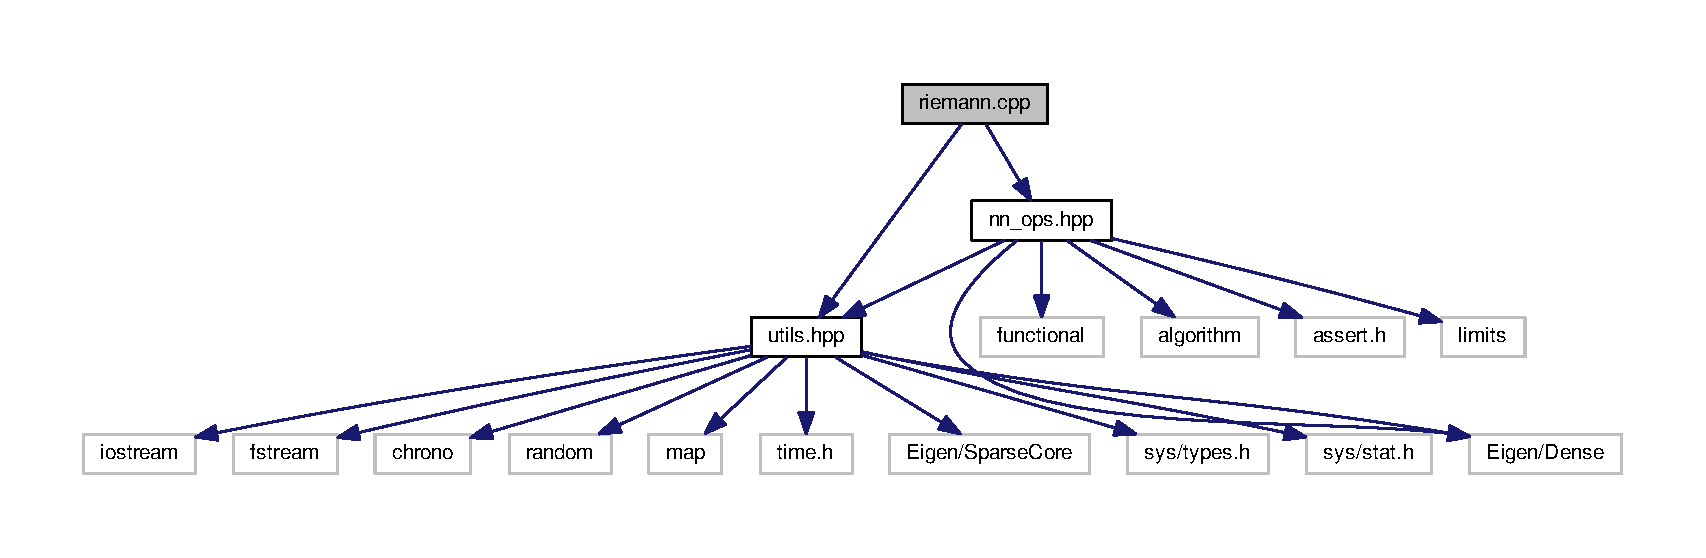
\includegraphics[width=350pt]{riemann_8cpp__incl}
\end{center}
\end{figure}
\subsection*{Functions}
\begin{DoxyCompactItemize}
\item 
\hypertarget{riemann_8cpp_a0ddf1224851353fc92bfbff6f499fa97}{}int {\bfseries main} (int argc, char $\ast$argv\mbox{[}$\,$\mbox{]})\label{riemann_8cpp_a0ddf1224851353fc92bfbff6f499fa97}

\end{DoxyCompactItemize}


\subsection{Detailed Description}
main function for launching experiments with neural networks 

\begin{DoxyAuthor}{Author}
Gaetan Marceau Caron \& Yann Ollivier 
\end{DoxyAuthor}
\begin{DoxyVersion}{Version}
1.\+0 
\end{DoxyVersion}

\hypertarget{utils_8hpp}{}\section{utils.\+hpp File Reference}
\label{utils_8hpp}\index{utils.\+hpp@{utils.\+hpp}}


Implementation of auxiliary functions required for dataset loading and outputting.  


{\ttfamily \#include $<$iostream$>$}\\*
{\ttfamily \#include $<$fstream$>$}\\*
{\ttfamily \#include $<$chrono$>$}\\*
{\ttfamily \#include $<$random$>$}\\*
{\ttfamily \#include $<$map$>$}\\*
{\ttfamily \#include $<$time.\+h$>$}\\*
{\ttfamily \#include $<$Eigen/\+Dense$>$}\\*
{\ttfamily \#include $<$Eigen/\+Sparse\+Core$>$}\\*
{\ttfamily \#include $<$sys/types.\+h$>$}\\*
{\ttfamily \#include $<$sys/stat.\+h$>$}\\*
Include dependency graph for utils.\+hpp\+:
\nopagebreak
\begin{figure}[H]
\begin{center}
\leavevmode
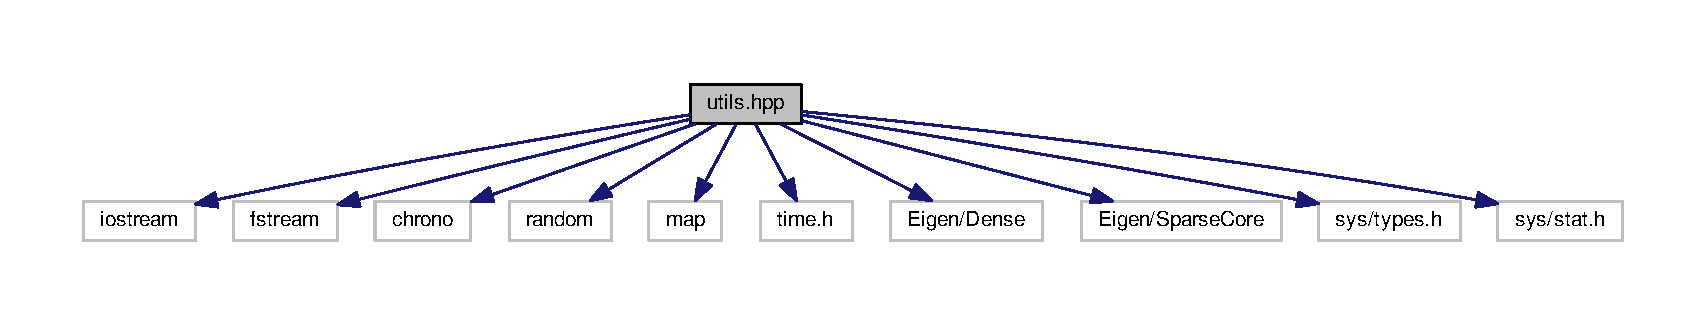
\includegraphics[width=350pt]{utils_8hpp__incl}
\end{center}
\end{figure}
This graph shows which files directly or indirectly include this file\+:
\nopagebreak
\begin{figure}[H]
\begin{center}
\leavevmode
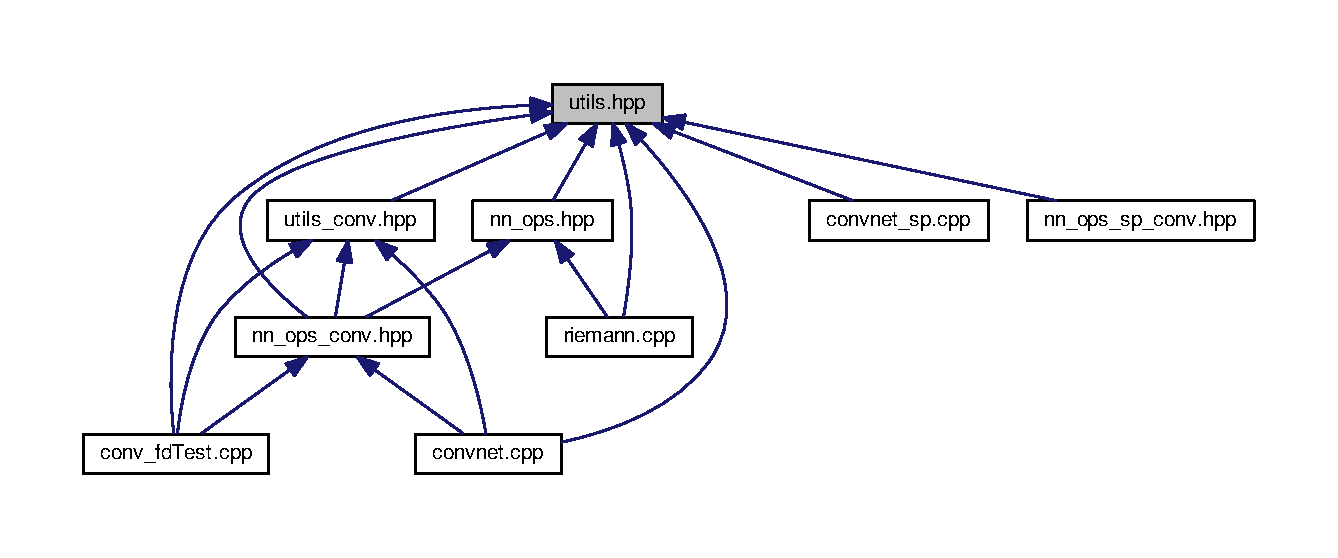
\includegraphics[width=350pt]{utils_8hpp__dep__incl}
\end{center}
\end{figure}
\subsection*{Classes}
\begin{DoxyCompactItemize}
\item 
struct \hyperlink{struct_params}{Params}
\end{DoxyCompactItemize}
\subsection*{Typedefs}
\begin{DoxyCompactItemize}
\item 
\hypertarget{utils_8hpp_a9383dd932a4b78622a7a1d2db5c82402}{}using {\bfseries My\+Sp\+Matrix} = Eigen\+::\+Sparse\+Matrix$<$ double, Col\+Major $>$\label{utils_8hpp_a9383dd932a4b78622a7a1d2db5c82402}

\item 
\hypertarget{utils_8hpp_af8f2e2685082c7a1ce52da465889378a}{}using {\bfseries My\+Matrix} = Eigen\+::\+Matrix$<$ double, Dynamic, Dynamic, Col\+Major $>$\label{utils_8hpp_af8f2e2685082c7a1ce52da465889378a}

\item 
\hypertarget{utils_8hpp_a16444aa6a902fc0ed5b34b5596aa37b7}{}using {\bfseries Sp\+Entry} = Eigen\+::\+Triplet$<$ double $>$\label{utils_8hpp_a16444aa6a902fc0ed5b34b5596aa37b7}

\item 
\hypertarget{utils_8hpp_af51a59f565b7450f96bf3fcf2e438c93}{}using {\bfseries My\+Vector} = Eigen\+::\+Matrix$<$ double, Dynamic, 1, Col\+Major $>$\label{utils_8hpp_af51a59f565b7450f96bf3fcf2e438c93}

\item 
\hypertarget{utils_8hpp_a436cf01a405728e59c24f8f0ca754a81}{}using {\bfseries Activation\+Function} = std\+::function$<$ void(const My\+Matrix \&, My\+Matrix \&, My\+Matrix \&)$>$\label{utils_8hpp_a436cf01a405728e59c24f8f0ca754a81}

\item 
\hypertarget{utils_8hpp_aa0c25e9c03997ebcd5aa6b837f671d9f}{}using {\bfseries Forward\+Function} = std\+::function$<$ void(const Activation\+Function \&, const std\+::vector$<$ My\+Matrix $>$ \&, const std\+::vector$<$ My\+Vector $>$ \&, const My\+Matrix \&, std\+::vector$<$ My\+Matrix $>$ \&, std\+::vector$<$ My\+Matrix $>$ \&, std\+::vector$<$ My\+Matrix $>$ \&)$>$\label{utils_8hpp_aa0c25e9c03997ebcd5aa6b837f671d9f}

\end{DoxyCompactItemize}
\subsection*{Functions}
\begin{DoxyCompactItemize}
\item 
\hypertarget{utils_8hpp_a8f4184801babfe7e55e142491371de67}{}void {\bfseries printtime} ()\label{utils_8hpp_a8f4184801babfe7e55e142491371de67}

\item 
\hypertarget{utils_8hpp_a1e327b035b2c95cf6ad856e9a518393e}{}double {\bfseries gettime} ()\label{utils_8hpp_a1e327b035b2c95cf6ad856e9a518393e}

\item 
int \hyperlink{utils_8hpp_a0a096ffad5fdb0a4a5e65356c9c86306}{Reverse\+Int} (const int i)
\begin{DoxyCompactList}\small\item\em Implementation of the change of encoding. \end{DoxyCompactList}\item 
void \hyperlink{utils_8hpp_a384799100357de20e8aeb55c7d1fac64}{parse\+Y\+A\+M\+L\+Seq} (const std\+::string seq\+\_\+str, std\+::vector$<$ unsigned $>$ \&seq)
\begin{DoxyCompactList}\small\item\em Parse a sequence of number given as a string. \end{DoxyCompactList}\item 
void \hyperlink{utils_8hpp_aa683093645a1f31ec9f1a0db9087f315}{read\+Args} (const int argc, char $\ast$argv\mbox{[}$\,$\mbox{]}, std\+::map$<$ std\+::string, std\+::string $>$ \&args)
\begin{DoxyCompactList}\small\item\em Parse the arguments from the command line. \end{DoxyCompactList}\item 
void \hyperlink{utils_8hpp_a6df4dc95a46aec52f95f8d7c0c7a30af}{set\+Params\+From\+Args} (std\+::map$<$ std\+::string, std\+::string $>$ \&args, \hyperlink{struct_params}{Params} \&params)
\begin{DoxyCompactList}\small\item\em Fill the params holder structure with a dictionnary of key/value strings. \end{DoxyCompactList}\item 
void \hyperlink{utils_8hpp_a5839158679f93bc5a833ecb09154adff}{set\+Params} (const std\+::string algo, std\+::map$<$ std\+::string, std\+::string $>$ args, \hyperlink{struct_params}{Params} \&params)
\begin{DoxyCompactList}\small\item\em Set the default parameters according to the chosen algorithm. \end{DoxyCompactList}\item 
void \hyperlink{utils_8hpp_a62ba4722350d9884660004d67199668d}{load\+Y\+A\+M\+L} (const std\+::string filename, std\+::map$<$ std\+::string, std\+::string $>$ \&config)
\begin{DoxyCompactList}\small\item\em Read the arguments from a Y\+A\+M\+L file. \end{DoxyCompactList}\item 
void \hyperlink{utils_8hpp_a0ee2ecc555aaa5b95a336c1d6b26a178}{set\+Params\+From\+File} (const std\+::string filename, std\+::map$<$ std\+::string, std\+::string $>$ \&args, \hyperlink{struct_params}{Params} \&params)
\begin{DoxyCompactList}\small\item\em Read the arguments and save them into the parameters holder structure. \end{DoxyCompactList}\item 
void \hyperlink{utils_8hpp_a96a1ff513794c047658d4bd461ff6add}{print\+Desc} (\hyperlink{struct_params}{Params} params, ostream $\ast$logger)
\begin{DoxyCompactList}\small\item\em print the description of the parameters \end{DoxyCompactList}\item 
void \hyperlink{utils_8hpp_a29b18fe301e0927dd6b955511b4f713b}{read\+M\+N\+I\+S\+T} (const string filename, My\+Matrix \&images, bool invert\+\_\+pixel)
\begin{DoxyCompactList}\small\item\em read the M\+N\+I\+S\+T images \end{DoxyCompactList}\item 
void \hyperlink{utils_8hpp_a02aa568999be47b9682eb358a6b1ae6e}{read\+M\+N\+I\+S\+T\+Label} (const string filename, My\+Vector \&labels)
\begin{DoxyCompactList}\small\item\em read the M\+N\+I\+S\+T labels \end{DoxyCompactList}\item 
int \hyperlink{utils_8hpp_a79f04d7f6ff9cd3caae4cdda562e5a01}{read\+C\+I\+F\+A\+R10} (const std\+::string filepath, My\+Matrix \&images, My\+Vector \&labels)
\begin{DoxyCompactList}\small\item\em read the C\+I\+F\+A\+R-\/10 images \end{DoxyCompactList}\item 
\hypertarget{utils_8hpp_a26e704ab3a2161fdc611f38ed0b2a11b}{}void {\bfseries load\+Light\+C\+I\+F\+A\+R10} (const double ratio\+\_\+train, My\+Matrix \&X\+\_\+train, My\+Matrix \&X\+\_\+valid, My\+Vector \&Y\+\_\+train, My\+Vector \&Y\+\_\+valid)\label{utils_8hpp_a26e704ab3a2161fdc611f38ed0b2a11b}

\item 
\hypertarget{utils_8hpp_afbdf4156cea7c6c2ace644e0f2944b85}{}void {\bfseries load\+C\+I\+F\+A\+R10} (const double ratio\+\_\+train, My\+Matrix \&X\+\_\+train, My\+Matrix \&X\+\_\+valid, My\+Vector \&Y\+\_\+train, My\+Vector \&Y\+\_\+valid)\label{utils_8hpp_afbdf4156cea7c6c2ace644e0f2944b85}

\item 
\hypertarget{utils_8hpp_a59b61ef932f6eefdfc8c2d0bd57d9d1f}{}void {\bfseries shuffle\+Database} (My\+Matrix \&data, My\+Vector \&labels, unsigned n\+\_\+examples=0)\label{utils_8hpp_a59b61ef932f6eefdfc8c2d0bd57d9d1f}

\item 
\hypertarget{utils_8hpp_aff3761117c5f33b7612c0a8c64850ab9}{}void {\bfseries load\+Mnist} (const \hyperlink{struct_params}{Params} \&params, My\+Matrix \&X\+\_\+train, My\+Matrix \&X\+\_\+valid, My\+Vector \&Y\+\_\+train, My\+Vector \&Y\+\_\+valid)\label{utils_8hpp_aff3761117c5f33b7612c0a8c64850ab9}

\item 
\hypertarget{utils_8hpp_abb66696c7dd025108b10bcf30cf88456}{}void {\bfseries get\+Mini\+Batch} (const unsigned j, const unsigned batch\+\_\+size, const My\+Matrix \&X, const Vector\+Xd \&Y, const My\+Matrix \&one\+\_\+hot, unsigned \&curr\+\_\+batch\+\_\+size, My\+Matrix \&X\+\_\+batch, My\+Matrix \&one\+\_\+hot\+\_\+batch)\label{utils_8hpp_abb66696c7dd025108b10bcf30cf88456}

\item 
\hypertarget{utils_8hpp_a8df68d69d0d6344f81e415e48354de4d}{}void {\bfseries labels2one\+Hot} (const My\+Matrix \&labels, My\+Matrix \&one\+\_\+hot)\label{utils_8hpp_a8df68d69d0d6344f81e415e48354de4d}

\item 
\hypertarget{utils_8hpp_aacccc5760793abdf7a59e73ef0159cae}{}void {\bfseries write\+Network} (const std\+::string filename, std\+::vector$<$ My\+Matrix $>$ \&W, std\+::vector$<$ My\+Vector $>$ \&B)\label{utils_8hpp_aacccc5760793abdf7a59e73ef0159cae}

\item 
\hypertarget{utils_8hpp_a7d0c5de4e2fd4062f369998b7ed6c72e}{}int {\bfseries load\+Network} (const std\+::string filename, std\+::vector$<$ My\+Matrix $>$ \&W, std\+::vector$<$ My\+Vector $>$ \&B)\label{utils_8hpp_a7d0c5de4e2fd4062f369998b7ed6c72e}

\item 
\hypertarget{utils_8hpp_ae5a82a442a3167a5f09592e391697883}{}void {\bfseries create\+Log\+Dir} (const std\+::string dir)\label{utils_8hpp_ae5a82a442a3167a5f09592e391697883}

\item 
\hypertarget{utils_8hpp_a01429fef023f0415731125356b2f6dec}{}void {\bfseries get\+Output} (const std\+::string path, ostream $\ast$\&out)\label{utils_8hpp_a01429fef023f0415731125356b2f6dec}

\item 
\hypertarget{utils_8hpp_a27ecc2ea0479ad392c5b9e46ad0fde1b}{}void {\bfseries monitor} (const std\+::vector$<$ My\+Matrix $>$ \&A\+\_\+vec)\label{utils_8hpp_a27ecc2ea0479ad392c5b9e46ad0fde1b}

\end{DoxyCompactItemize}
\subsection*{Variables}
\begin{DoxyCompactItemize}
\item 
\hypertarget{utils_8hpp_ab49a616e1496272eef0037cdfe03f98b}{}const std\+::string {\bfseries C\+I\+F\+A\+R\+\_\+\+D\+I\+R} = \char`\"{}./cifar-\/10-\/batches-\/bin/\char`\"{}\label{utils_8hpp_ab49a616e1496272eef0037cdfe03f98b}

\item 
\hypertarget{utils_8hpp_a77e6d9c658f7dea0b529984c9075f50b}{}const std\+::string {\bfseries M\+N\+I\+S\+T\+\_\+\+D\+I\+R} = \char`\"{}./mnist/\char`\"{}\label{utils_8hpp_a77e6d9c658f7dea0b529984c9075f50b}

\item 
\hypertarget{utils_8hpp_a1eaf6cedc54267bfff99f2700b0f8c2d}{}const unsigned {\bfseries N\+\_\+\+R\+O\+W} = 10000\label{utils_8hpp_a1eaf6cedc54267bfff99f2700b0f8c2d}

\item 
\hypertarget{utils_8hpp_a37ea3403219151fb6f509ee7ed571d7e}{}const unsigned {\bfseries N\+\_\+\+C\+H\+A\+N\+N\+E\+L} = 1\label{utils_8hpp_a37ea3403219151fb6f509ee7ed571d7e}

\item 
\hypertarget{utils_8hpp_aeb1ed8e1604c6b7268fd1bef57d0be70}{}const unsigned {\bfseries I\+M\+G\+\_\+\+W\+I\+D\+T\+H} = 28\label{utils_8hpp_aeb1ed8e1604c6b7268fd1bef57d0be70}

\item 
\hypertarget{utils_8hpp_af9f8e327af39cfb5f166889109a51689}{}const unsigned {\bfseries I\+M\+G\+\_\+\+H\+E\+I\+G\+H\+T} = 28\label{utils_8hpp_af9f8e327af39cfb5f166889109a51689}

\item 
\hypertarget{utils_8hpp_ae3fc053a24d81b793719a04bc1b7c47b}{}const unsigned {\bfseries N\+\_\+\+P\+I\+X\+E\+L} = I\+M\+G\+\_\+\+W\+I\+D\+T\+H $\ast$ I\+M\+G\+\_\+\+H\+E\+I\+G\+H\+T\label{utils_8hpp_ae3fc053a24d81b793719a04bc1b7c47b}

\item 
\hypertarget{utils_8hpp_ab577cbc7a7051e1bcf60c2c1797a0feb}{}std\+::mt19937 {\bfseries gen}\label{utils_8hpp_ab577cbc7a7051e1bcf60c2c1797a0feb}

\item 
\hypertarget{utils_8hpp_a651bb0654263299f2b7d5164e409174d}{}auto {\bfseries t} =clock()\label{utils_8hpp_a651bb0654263299f2b7d5164e409174d}

\item 
\hypertarget{utils_8hpp_abc867299ce5e1817c1bf020588f2e885}{}auto {\bfseries starting\+\_\+time} =clock()\label{utils_8hpp_abc867299ce5e1817c1bf020588f2e885}

\end{DoxyCompactItemize}


\subsection{Detailed Description}
Implementation of auxiliary functions required for dataset loading and outputting. 

Implementation of auxiliary functions for dataset loading, parameter handling and outputting.

\begin{DoxyAuthor}{Author}
Gaetan Marceau Caron \& Yann Ollivier 
\end{DoxyAuthor}
\begin{DoxyVersion}{Version}
1.\+0 
\end{DoxyVersion}


\subsection{Function Documentation}
\hypertarget{utils_8hpp_a62ba4722350d9884660004d67199668d}{}\index{utils.\+hpp@{utils.\+hpp}!load\+Y\+A\+M\+L@{load\+Y\+A\+M\+L}}
\index{load\+Y\+A\+M\+L@{load\+Y\+A\+M\+L}!utils.\+hpp@{utils.\+hpp}}
\subsubsection[{load\+Y\+A\+M\+L}]{\setlength{\rightskip}{0pt plus 5cm}void load\+Y\+A\+M\+L (
\begin{DoxyParamCaption}
\item[{const std\+::string}]{filename, }
\item[{std\+::map$<$ std\+::string, std\+::string $>$ \&}]{config}
\end{DoxyParamCaption}
)}\label{utils_8hpp_a62ba4722350d9884660004d67199668d}


Read the arguments from a Y\+A\+M\+L file. 


\begin{DoxyParams}{Parameters}
{\em filename} & the path of the Y\+A\+M\+L file \\
\hline
{\em config} & a map containing pairs of key/value strings \\
\hline
\end{DoxyParams}
\hypertarget{utils_8hpp_a384799100357de20e8aeb55c7d1fac64}{}\index{utils.\+hpp@{utils.\+hpp}!parse\+Y\+A\+M\+L\+Seq@{parse\+Y\+A\+M\+L\+Seq}}
\index{parse\+Y\+A\+M\+L\+Seq@{parse\+Y\+A\+M\+L\+Seq}!utils.\+hpp@{utils.\+hpp}}
\subsubsection[{parse\+Y\+A\+M\+L\+Seq}]{\setlength{\rightskip}{0pt plus 5cm}void parse\+Y\+A\+M\+L\+Seq (
\begin{DoxyParamCaption}
\item[{const std\+::string}]{seq\+\_\+str, }
\item[{std\+::vector$<$ unsigned $>$ \&}]{seq}
\end{DoxyParamCaption}
)}\label{utils_8hpp_a384799100357de20e8aeb55c7d1fac64}


Parse a sequence of number given as a string. 


\begin{DoxyParams}{Parameters}
{\em seq\+\_\+str} & the string to parse \\
\hline
{\em seq} & the vector of numbers \\
\hline
\end{DoxyParams}
\hypertarget{utils_8hpp_a96a1ff513794c047658d4bd461ff6add}{}\index{utils.\+hpp@{utils.\+hpp}!print\+Desc@{print\+Desc}}
\index{print\+Desc@{print\+Desc}!utils.\+hpp@{utils.\+hpp}}
\subsubsection[{print\+Desc}]{\setlength{\rightskip}{0pt plus 5cm}void print\+Desc (
\begin{DoxyParamCaption}
\item[{{\bf Params}}]{params, }
\item[{ostream $\ast$}]{logger}
\end{DoxyParamCaption}
)}\label{utils_8hpp_a96a1ff513794c047658d4bd461ff6add}


print the description of the parameters 


\begin{DoxyParams}{Parameters}
{\em params} & a param holder structure \\
\hline
{\em logger} & the output stream to print on \\
\hline
\end{DoxyParams}
\hypertarget{utils_8hpp_aa683093645a1f31ec9f1a0db9087f315}{}\index{utils.\+hpp@{utils.\+hpp}!read\+Args@{read\+Args}}
\index{read\+Args@{read\+Args}!utils.\+hpp@{utils.\+hpp}}
\subsubsection[{read\+Args}]{\setlength{\rightskip}{0pt plus 5cm}void read\+Args (
\begin{DoxyParamCaption}
\item[{const int}]{argc, }
\item[{char $\ast$}]{argv\mbox{[}$\,$\mbox{]}, }
\item[{std\+::map$<$ std\+::string, std\+::string $>$ \&}]{args}
\end{DoxyParamCaption}
)}\label{utils_8hpp_aa683093645a1f31ec9f1a0db9087f315}


Parse the arguments from the command line. 


\begin{DoxyParams}{Parameters}
{\em argc} & the number of arguments to parse \\
\hline
{\em argv} & the vector of arguments given as strings \\
\hline
{\em args} & a map containing pairs of key/value strings \\
\hline
\end{DoxyParams}
\hypertarget{utils_8hpp_a79f04d7f6ff9cd3caae4cdda562e5a01}{}\index{utils.\+hpp@{utils.\+hpp}!read\+C\+I\+F\+A\+R10@{read\+C\+I\+F\+A\+R10}}
\index{read\+C\+I\+F\+A\+R10@{read\+C\+I\+F\+A\+R10}!utils.\+hpp@{utils.\+hpp}}
\subsubsection[{read\+C\+I\+F\+A\+R10}]{\setlength{\rightskip}{0pt plus 5cm}int read\+C\+I\+F\+A\+R10 (
\begin{DoxyParamCaption}
\item[{const std\+::string}]{filepath, }
\item[{My\+Matrix \&}]{images, }
\item[{My\+Vector \&}]{labels}
\end{DoxyParamCaption}
)}\label{utils_8hpp_a79f04d7f6ff9cd3caae4cdda562e5a01}


read the C\+I\+F\+A\+R-\/10 images 


\begin{DoxyParams}{Parameters}
{\em images} & the design matrix of the images \\
\hline
{\em labels} & the labels associated to the images (same order than previous function) \\
\hline
\end{DoxyParams}
\hypertarget{utils_8hpp_a29b18fe301e0927dd6b955511b4f713b}{}\index{utils.\+hpp@{utils.\+hpp}!read\+M\+N\+I\+S\+T@{read\+M\+N\+I\+S\+T}}
\index{read\+M\+N\+I\+S\+T@{read\+M\+N\+I\+S\+T}!utils.\+hpp@{utils.\+hpp}}
\subsubsection[{read\+M\+N\+I\+S\+T}]{\setlength{\rightskip}{0pt plus 5cm}void read\+M\+N\+I\+S\+T (
\begin{DoxyParamCaption}
\item[{const string}]{filename, }
\item[{My\+Matrix \&}]{images, }
\item[{bool}]{invert\+\_\+pixel}
\end{DoxyParamCaption}
)}\label{utils_8hpp_a29b18fe301e0927dd6b955511b4f713b}


read the M\+N\+I\+S\+T images 


\begin{DoxyParams}{Parameters}
{\em filename} & the filename of the M\+N\+I\+S\+T data file \\
\hline
{\em images} & the design matrix of the images \\
\hline
{\em invert\+\_\+pixel} & a flag to invert the pixel of the images \\
\hline
\end{DoxyParams}
\hypertarget{utils_8hpp_a02aa568999be47b9682eb358a6b1ae6e}{}\index{utils.\+hpp@{utils.\+hpp}!read\+M\+N\+I\+S\+T\+Label@{read\+M\+N\+I\+S\+T\+Label}}
\index{read\+M\+N\+I\+S\+T\+Label@{read\+M\+N\+I\+S\+T\+Label}!utils.\+hpp@{utils.\+hpp}}
\subsubsection[{read\+M\+N\+I\+S\+T\+Label}]{\setlength{\rightskip}{0pt plus 5cm}void read\+M\+N\+I\+S\+T\+Label (
\begin{DoxyParamCaption}
\item[{const string}]{filename, }
\item[{My\+Vector \&}]{labels}
\end{DoxyParamCaption}
)}\label{utils_8hpp_a02aa568999be47b9682eb358a6b1ae6e}


read the M\+N\+I\+S\+T labels 


\begin{DoxyParams}{Parameters}
{\em filename} & the filename of the M\+N\+I\+S\+T data file \\
\hline
{\em labels} & the labels associated to the images (same order than previous function) \\
\hline
\end{DoxyParams}
\hypertarget{utils_8hpp_a0a096ffad5fdb0a4a5e65356c9c86306}{}\index{utils.\+hpp@{utils.\+hpp}!Reverse\+Int@{Reverse\+Int}}
\index{Reverse\+Int@{Reverse\+Int}!utils.\+hpp@{utils.\+hpp}}
\subsubsection[{Reverse\+Int}]{\setlength{\rightskip}{0pt plus 5cm}int Reverse\+Int (
\begin{DoxyParamCaption}
\item[{const int}]{i}
\end{DoxyParamCaption}
)}\label{utils_8hpp_a0a096ffad5fdb0a4a5e65356c9c86306}


Implementation of the change of encoding. 


\begin{DoxyParams}{Parameters}
{\em i} & the variable to transform \\
\hline
\end{DoxyParams}
\begin{DoxyReturn}{Returns}
the transformed variable 
\end{DoxyReturn}
\hypertarget{utils_8hpp_a5839158679f93bc5a833ecb09154adff}{}\index{utils.\+hpp@{utils.\+hpp}!set\+Params@{set\+Params}}
\index{set\+Params@{set\+Params}!utils.\+hpp@{utils.\+hpp}}
\subsubsection[{set\+Params}]{\setlength{\rightskip}{0pt plus 5cm}void set\+Params (
\begin{DoxyParamCaption}
\item[{const std\+::string}]{algo, }
\item[{std\+::map$<$ std\+::string, std\+::string $>$}]{args, }
\item[{{\bf Params} \&}]{params}
\end{DoxyParamCaption}
)}\label{utils_8hpp_a5839158679f93bc5a833ecb09154adff}


Set the default parameters according to the chosen algorithm. 


\begin{DoxyParams}{Parameters}
{\em algo} & the name of the algorithm \\
\hline
{\em args} & a map containing pairs of key/value strings \\
\hline
{\em params} & a param holder structure \\
\hline
\end{DoxyParams}
\hypertarget{utils_8hpp_a6df4dc95a46aec52f95f8d7c0c7a30af}{}\index{utils.\+hpp@{utils.\+hpp}!set\+Params\+From\+Args@{set\+Params\+From\+Args}}
\index{set\+Params\+From\+Args@{set\+Params\+From\+Args}!utils.\+hpp@{utils.\+hpp}}
\subsubsection[{set\+Params\+From\+Args}]{\setlength{\rightskip}{0pt plus 5cm}void set\+Params\+From\+Args (
\begin{DoxyParamCaption}
\item[{std\+::map$<$ std\+::string, std\+::string $>$ \&}]{args, }
\item[{{\bf Params} \&}]{params}
\end{DoxyParamCaption}
)}\label{utils_8hpp_a6df4dc95a46aec52f95f8d7c0c7a30af}


Fill the params holder structure with a dictionnary of key/value strings. 


\begin{DoxyParams}{Parameters}
{\em args} & a map containing pairs of key/value strings \\
\hline
{\em params} & a param holder structure \\
\hline
\end{DoxyParams}
\hypertarget{utils_8hpp_a0ee2ecc555aaa5b95a336c1d6b26a178}{}\index{utils.\+hpp@{utils.\+hpp}!set\+Params\+From\+File@{set\+Params\+From\+File}}
\index{set\+Params\+From\+File@{set\+Params\+From\+File}!utils.\+hpp@{utils.\+hpp}}
\subsubsection[{set\+Params\+From\+File}]{\setlength{\rightskip}{0pt plus 5cm}void set\+Params\+From\+File (
\begin{DoxyParamCaption}
\item[{const std\+::string}]{filename, }
\item[{std\+::map$<$ std\+::string, std\+::string $>$ \&}]{args, }
\item[{{\bf Params} \&}]{params}
\end{DoxyParamCaption}
)}\label{utils_8hpp_a0ee2ecc555aaa5b95a336c1d6b26a178}


Read the arguments and save them into the parameters holder structure. 


\begin{DoxyParams}{Parameters}
{\em filename} & the path of the Y\+A\+M\+L file \\
\hline
{\em args} & a map containing pairs of key/value strings \\
\hline
{\em params} & a param holder structure \\
\hline
\end{DoxyParams}

%--- End generated contents ---

% Index
\backmatter
\newpage
\phantomsection
\clearemptydoublepage
\addcontentsline{toc}{chapter}{Index}
\printindex

\end{document}
